\documentclass[12pt, landscape]{article}
\usepackage[scaled=0.92]{helvet}
\usepackage{multicol}
\usepackage{calc}
\usepackage{ifthen}
% \usepackage[a4paper, total={6in, 8in}]{geometry}
\usepackage[landscape]{geometry}
%\usepackage{hyperref}

\usepackage{newtxtext} 

%for strikeout
\usepackage{ulem}

%For editing parbox
\usepackage[table]{xcolor}
%For editing itemise margins, reduce iterm separaion and list separation
\usepackage{enumitem}
% For math
\usepackage{amsmath,amsthm,amsfonts,amssymb}

%For pictures / figures
\usepackage{color,graphicx,overpic}
\graphicspath{ {./images/} }

%\usepackage{newtxtext} 
%\usepackage{amssymb}
%\usepackage[table]{xcolor}
%\usepackage{vwcol}
%\usepackage{tikz}
%\usepackage{wrapfig}
%\usepackage{makecell}


% For Code Blocks
\usepackage{xcolor}
\usepackage{listings}

% C++ Code Blocks:
\definecolor{listinggray}{gray}{0.9}
\definecolor{lbcolor}{rgb}{0.9,0.9,0.9}
\definecolor{Darkgreen}{rgb}{0,0.4,0}
\lstset{
    backgroundcolor=\color{lbcolor},
    tabsize=4,    
%   rulecolor=,
    language=[GNU]C++,
        basicstyle=\tiny,
        upquote=true,
        aboveskip={0.5\baselineskip},
	% Represents top margin
        columns=fixed,
        showstringspaces=false,
        extendedchars=false,
        breaklines=true,
        prebreak = \raisebox{0ex}[0ex][0ex]{\ensuremath{\hookleftarrow}},
        frame=single,
	% Remove Numbers
        numbers=none,
        showtabs=false,
        showspaces=false,
        showstringspaces=false,
        identifierstyle=\ttfamily,
        keywordstyle=\color[rgb]{0,0,1},
        commentstyle=\color[rgb]{0.026,0.112,0.095},
        stringstyle=\color[rgb]{0.627,0.126,0.941},
        % numberstyle=\color[rgb]{0.205, 0.142, 0.73},
%        \lstdefinestyle{C++}{language=C++,style=numbers}’.
}
\lstset{
    backgroundcolor=\color{lbcolor},
    tabsize=4,
  language=C++,
  captionpos=b,
  tabsize=3,
  frame=lines,
  % Remove Numbers
  numbers=none,
  numberstyle=\tiny,
  numbersep=3 pt,
  breaklines=true,
  showstringspaces=false,
  basicstyle=\tiny,
%  identifierstyle=\color{magenta},
  keywordstyle=\color[rgb]{0,0,1},
  commentstyle=\color{Darkgreen},
  stringstyle=\color{red}
}
% \lstset{language=C++}
%% Different languages: SQL, C++, Python


%Helpful:
%[linewidth = 1.0 \linewidth]
%\lstinline{}
% use \code{} for \lstinline with colorbox.
\newcommand{\code}[1]{\colorbox{gray!25!}{\lstinline[basicstyle=\scriptsize]|#1|}}

% Template: Cheatsheet with code enabled

%--------------------------- PACKAGES ABOVE --------------------------------------------------------------

\pdfinfo{
  /Title (CS2100 Summary.pdf)
  /Creator (Ger Teck)
  /Author (Ger Teck)
  /Subject ()
  /Keywords (tex)}

%% Margins for PAPER

% This sets page margins to .5 inch if using letter paper, and to 1cm
% if using A4 paper. (This probably isn't strictly necessary.)
% If using another size paper, use default 1cm margins.
\ifthenelse{\lengthtest { \paperwidth = 11in}}
	{ \geometry{top=.3in,left=.3in,right=.3in,bottom=.3in} }
	{\ifthenelse{ \lengthtest{ \paperwidth = 297mm}}
		{\geometry{top=0.5cm,left=0.5cm,right=0.5cm,bottom=0.5cm} }
		{\geometry{top=0.5cm,left=0.5cm,right=0.5cm,bottom=0.5cm} }
	}

% Turn off header and footer
\pagestyle{empty}

% for tight centres (less spacing)
\newenvironment{tightcenter}{%
  \setlength\topsep{0.5pt}
  \setlength\parskip{0.5pt}
  \begin{center}
}{%
  \end{center}
}

% Redefine section commands to use less space
\makeatletter
\renewcommand{\section}{\@startsection{section}{1}{0mm}%
                                {-1ex plus -.5ex minus -.2ex}%
                                {0.5ex plus .2ex}%x
                                {\normalfont\large\bfseries}}
\renewcommand{\subsection}{\@startsection{subsection}{2}{0mm}%
                                {-1explus -.5ex minus -.2ex}%
                                {0.5ex plus .2ex}%
                                {\normalfont\normalsize\bfseries}}
\renewcommand{\subsubsection}{\@startsection{subsubsection}{3}{0mm}%
                                {-1ex plus -.5ex minus -.2ex}%
                                {1ex plus .2ex}%
                                {\normalfont\small\bfseries}}
% change font
%\renewcommand{\familydefault}{\sfdefault}
%\renewcommand\rmdefault{\sfdefault}
\linespread{1.05}

\makeatother

% Define BibTeX command
\def\BibTeX{{\rm B\kern-.05em{\sc i\kern-.025em b}\kern-.08em
    T\kern-.1667em\lower.7ex\hbox{E}\kern-.125emX}}

% Don't print section numbers
\setcounter{secnumdepth}{0}

\setlength{\parindent}{0pt}
\setlength{\parskip}{0pt plus 0.5ex}

%% this changes all items (enumerate and itemize, reduce margins) ITEMIZE SEPARATION HERE
\setlength{\leftmargini}{0.5cm}
\setlength{\leftmarginii}{0.5cm}
\setlist[itemize,1]{leftmargin=2mm,labelindent=1mm,labelsep=1mm, itemsep = 0mm}
\setlist[itemize,2]{leftmargin=4mm,labelindent=1mm,labelsep=1mm, itemsep = 0mm}
%itemsep = 0mm
%\setlist{nosep}

% Need Logo Picture
%Watermark Top Right
%\usepackage{atbegshi,picture}
%\AtBeginShipout{\AtBeginShipoutUpperLeft{%
 % \put(\dimexpr\paperwidth-1.2cm\relax, -1.2cm){\makebox[0pt][r]{\framebox{
\includegraphics[width = 0.3cm]{mountainbooks} Ger Teck}}}%
%}}

% Justify Package
\usepackage[document]{ragged2e}

% -------------------------------------------------------------------------------

% START OF DOCUMENT HERE

\begin{document}
\raggedright
\footnotesize
\begin{multicols*}{3}



% multicol parameters
% These lengths are set only within the two main columns
%\setlength{\columnseprule}{0.25pt}
\setlength{\premulticols}{1pt}
\setlength{\postmulticols}{1pt}
\setlength{\multicolsep}{1pt}
\setlength{\columnsep}{2pt}

%% DOCUMENT NAME HERE
\begin{center}
     \Large{\textbf{CS2100 Comp Org Notes}} \\
\end{center}
AY23/24 Sem 1, github.com/gerteck

\section{12. Boolean Algebra}
\subsubsection{Digital Circuits}
\begin{itemize}
\item Two voltage levels, 1 for high, 0 for low.
\item Digital circuits over analog circuits are more reliable, specified accurarcy (determinable).
\item Digital circuits abstracted using simple mathematical model: \textbf{(Boolean Algebra)}
\item Design, Analysis and simplification of digital circuit: \textbf{Digital Logic Design.}
\item \textbf{Combinational}: no memory, output depends solely on the input. (gates, adders, multiplexers)
\item \textbf{Sequential:} with memory, output depends on both input and current state. (counters, registers, memories)
\end{itemize}

\subsubsection{Boolean Algebra}
connectives in order of precedence:
\begin{itemize}
\item \textbf{negation} $A'$ equivalent to \textbf{NOT}
\item \textbf{conjunction} $A \cdot B $ equivalent to \textbf{AND}
\item \textbf{disjunction} $ A + B $ equivalent to \textbf{OR}
\item Note: always write the AND operator $ \cdot $, do not omit, as it may be confused with a 2 bit value, $AB$.
\item \textbf{Truth Table}: Provides listing of every possible combination of inputs and corresponding outputs. We may prove using truth table by comparing columns.
\end{itemize}

\subsubsection{Duality}
\begin{itemize}
\item \textbf{Duality}: if the AND/OR operators and identity elements 0/1 interchanged in a boolean equation, it remains valid.
\item e.g. the dual equation of $a+(b\cdot c)=(a+b)\cdot(a+c)$ is  $a\cdot(b+c)=(a\cdot b)+(a\cdot c).$, where if one is valid, then its dual is also valid.
\end{itemize}



\subsubsection{Laws \& Theorems of Boolean Algebra}
\centerline{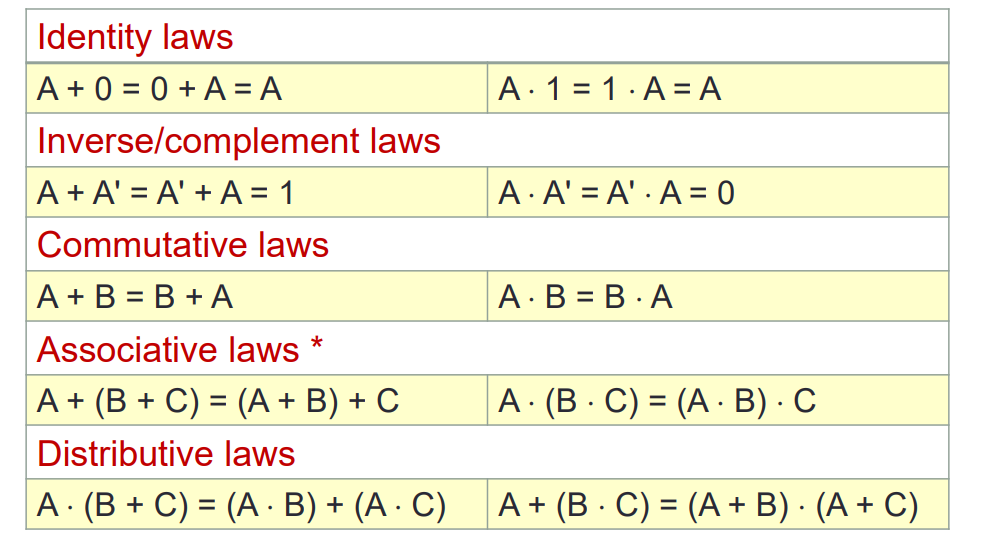
\includegraphics[width=1\linewidth]{BAlaw1}}
\bigskip
\centerline{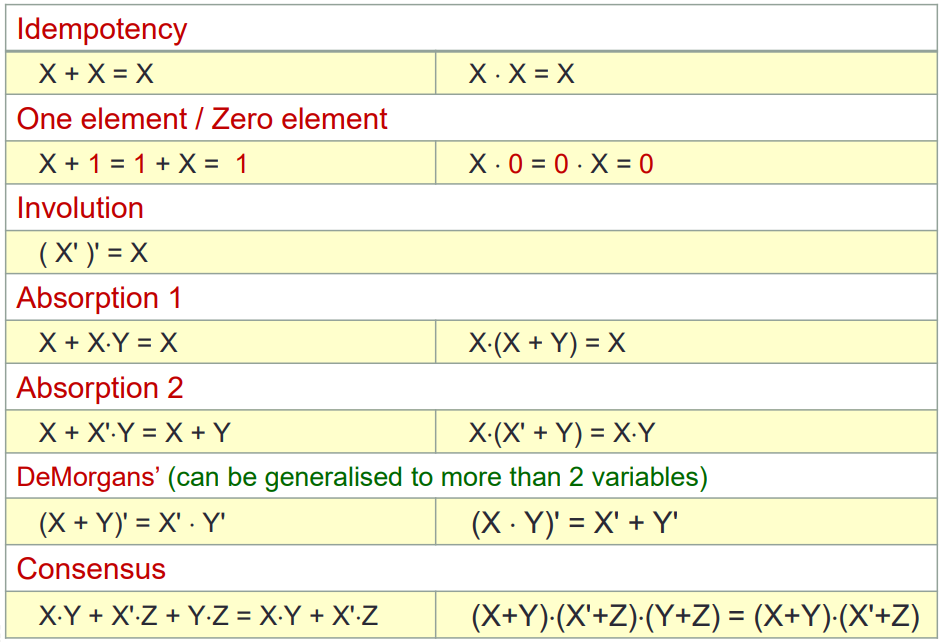
\includegraphics[width=1\linewidth]{BAlaw2}}
left/right equations are duals of each other

\subsubsection{Proving Theorems}
\begin{itemize}
\item Theorems can be proved using truth table, or by 
algebraic manipulation using other theorems/laws.
\end{itemize}
\centerline{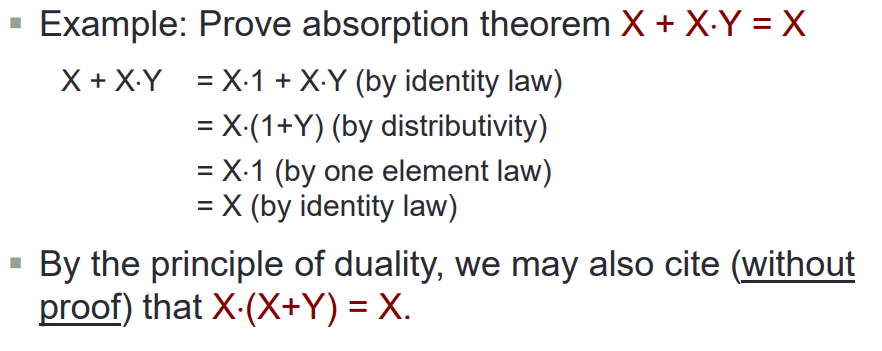
\includegraphics[width=0.5\linewidth]{prove}}

\subsubsection{Boolean Functions, Complements}
\begin{itemize}
\item Represented by $F$, e.g. $F1(x,y,z) = x\cdot y\cdot z'$.
\item To prove $F1 = F2$, we may use boolean algebra, or use truth tables.
\item Complement Function is denoted as $F'$, obtained by interchanging 1 with 0 in function's output values.
\end{itemize}

% \vfill \null
\columnbreak

\subsubsection{Standard Forms}
\begin{itemize}
\item \textbf{Literals}: A Boolean variable on its own or in its complemented form. (e.g. $x$, $x'$)
\item \textbf{Product Term}: A single literal or a logical product (AND, $\cdot$) of several literals. (e.g. $x$, $x \cdot y \cdot z'$ )
\item \textbf{Sum Term}: A single literal or a logical sum (OR $+$) of several literals. (e.g. $A + B'$)
\item \textbf{sum-of-products (SOP) expression}: A product term or a logical sum (OR $+$) of several product terms.
\item \textbf{product-of-sums (POS) expression}: A sum term or a logical product (AND) of several sum terms.
\item Every boolean expr can be expressed in SOP/POS form.
\end{itemize}

\subsubsection{Minterms and Maxterms}
\begin{itemize}
\item \textbf{minterm} (of n variables): a product term that contains n literals from all the variables; denoted $m0$ to $m[2^n - 1]$
\item \textbf{maxterm} (of n variables): a sum term that contains n literals from all the variables; denoted $M0$ to $M[2^n - 1]$ 
\item Each minterm is the complement ($m2' = M2$) of its corresponding maxterm, vice versa.
\end{itemize}
\centerline{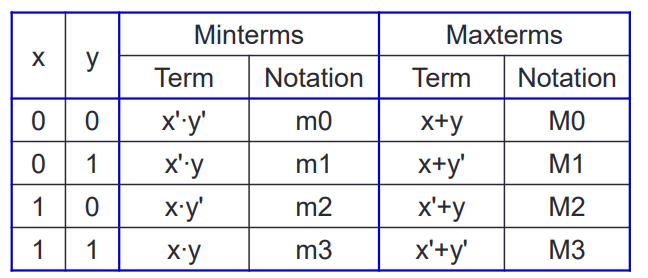
\includegraphics[width=0.5\linewidth]{minmax}}

\subsubsection{Canonical Forms}
\begin{itemize}
\item Canonical/normal form: a unique form of representation.
\item \textbf{Sum-of-minterms} = Canonical sum-of-products
\item \textbf{Product-of-maxterms} = Canonical product-of-sums
\end{itemize}
\centerline{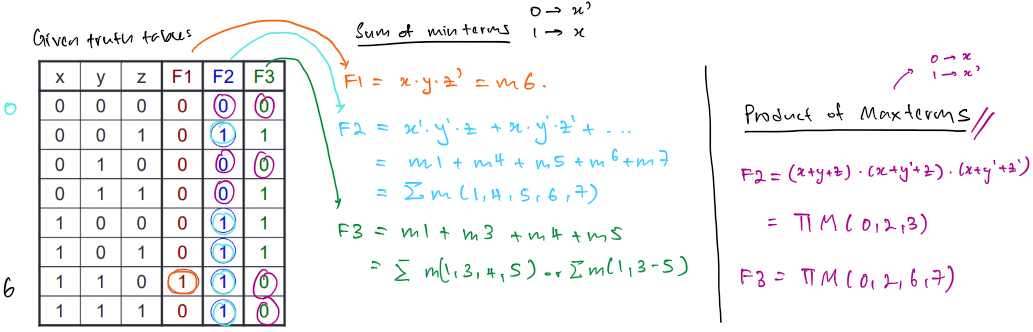
\includegraphics[width=1\linewidth]{canon}}
• We can convert between sum-of-minterms and product-of-maxterms easily, by DeMorgan's.

\section{13. Logic Gates \& Simplification}
\subsubsection{Logic Gates}
\begin{itemize}
\item Fan-in: The number of inputs of a gate $\geq$ 1, 2. 
\item Implement bool exp / function as logic circuit.
\end{itemize}

\subsubsection{Universal Gates}
\begin{itemize}
\item \textbf{universal gate}: can implement a complete set of logic.
\item $\{AND, OR, NOT\}$ are a complete set of logic, sufficient for building any boolean function.
\item $\{NAND\}$ and $\{NOR\}$ themselves a complete set of logic. Implement NOT/AND/OR using only NAND or NOR gates.
\end{itemize}

\subsubsection{SOP and POS}
\begin{itemize}
\item an SOP expression can be easily implemented using \\
◦ 2-level AND-OR circuit or 2-level NAND circuit
\item a POS expression can be easily implemented using \\
◦ 2-level OR-AND circuit or 2-level NOR circuit
\end{itemize}

\subsubsection{Algebraic Simplification}
\begin{itemize}
\item \textbf{Function Simplification}: Make use of alegbraic (using theorems) or Karnaugh Maps (easier to use, limited to no more than 6 variables) or Quine-McCluskey.
\item \textbf{Algebraic Simplification}: aims to minimise \\
1. number of literals (prioritised over number of terms) \\
2. number of terms.
\end{itemize}

\subsubsection{Half Adder}
\begin{itemize}
\item Half adder is a circuit that adds 2 single bits (X, Y) to produce a result of 2 bits (C, S).
\centerline{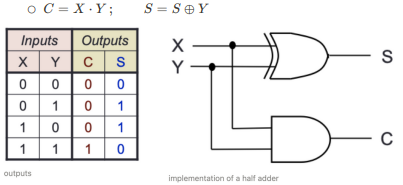
\includegraphics[width=1\linewidth]{halfadder}}
\end{itemize}

\section{Universal Gates}
\centerline{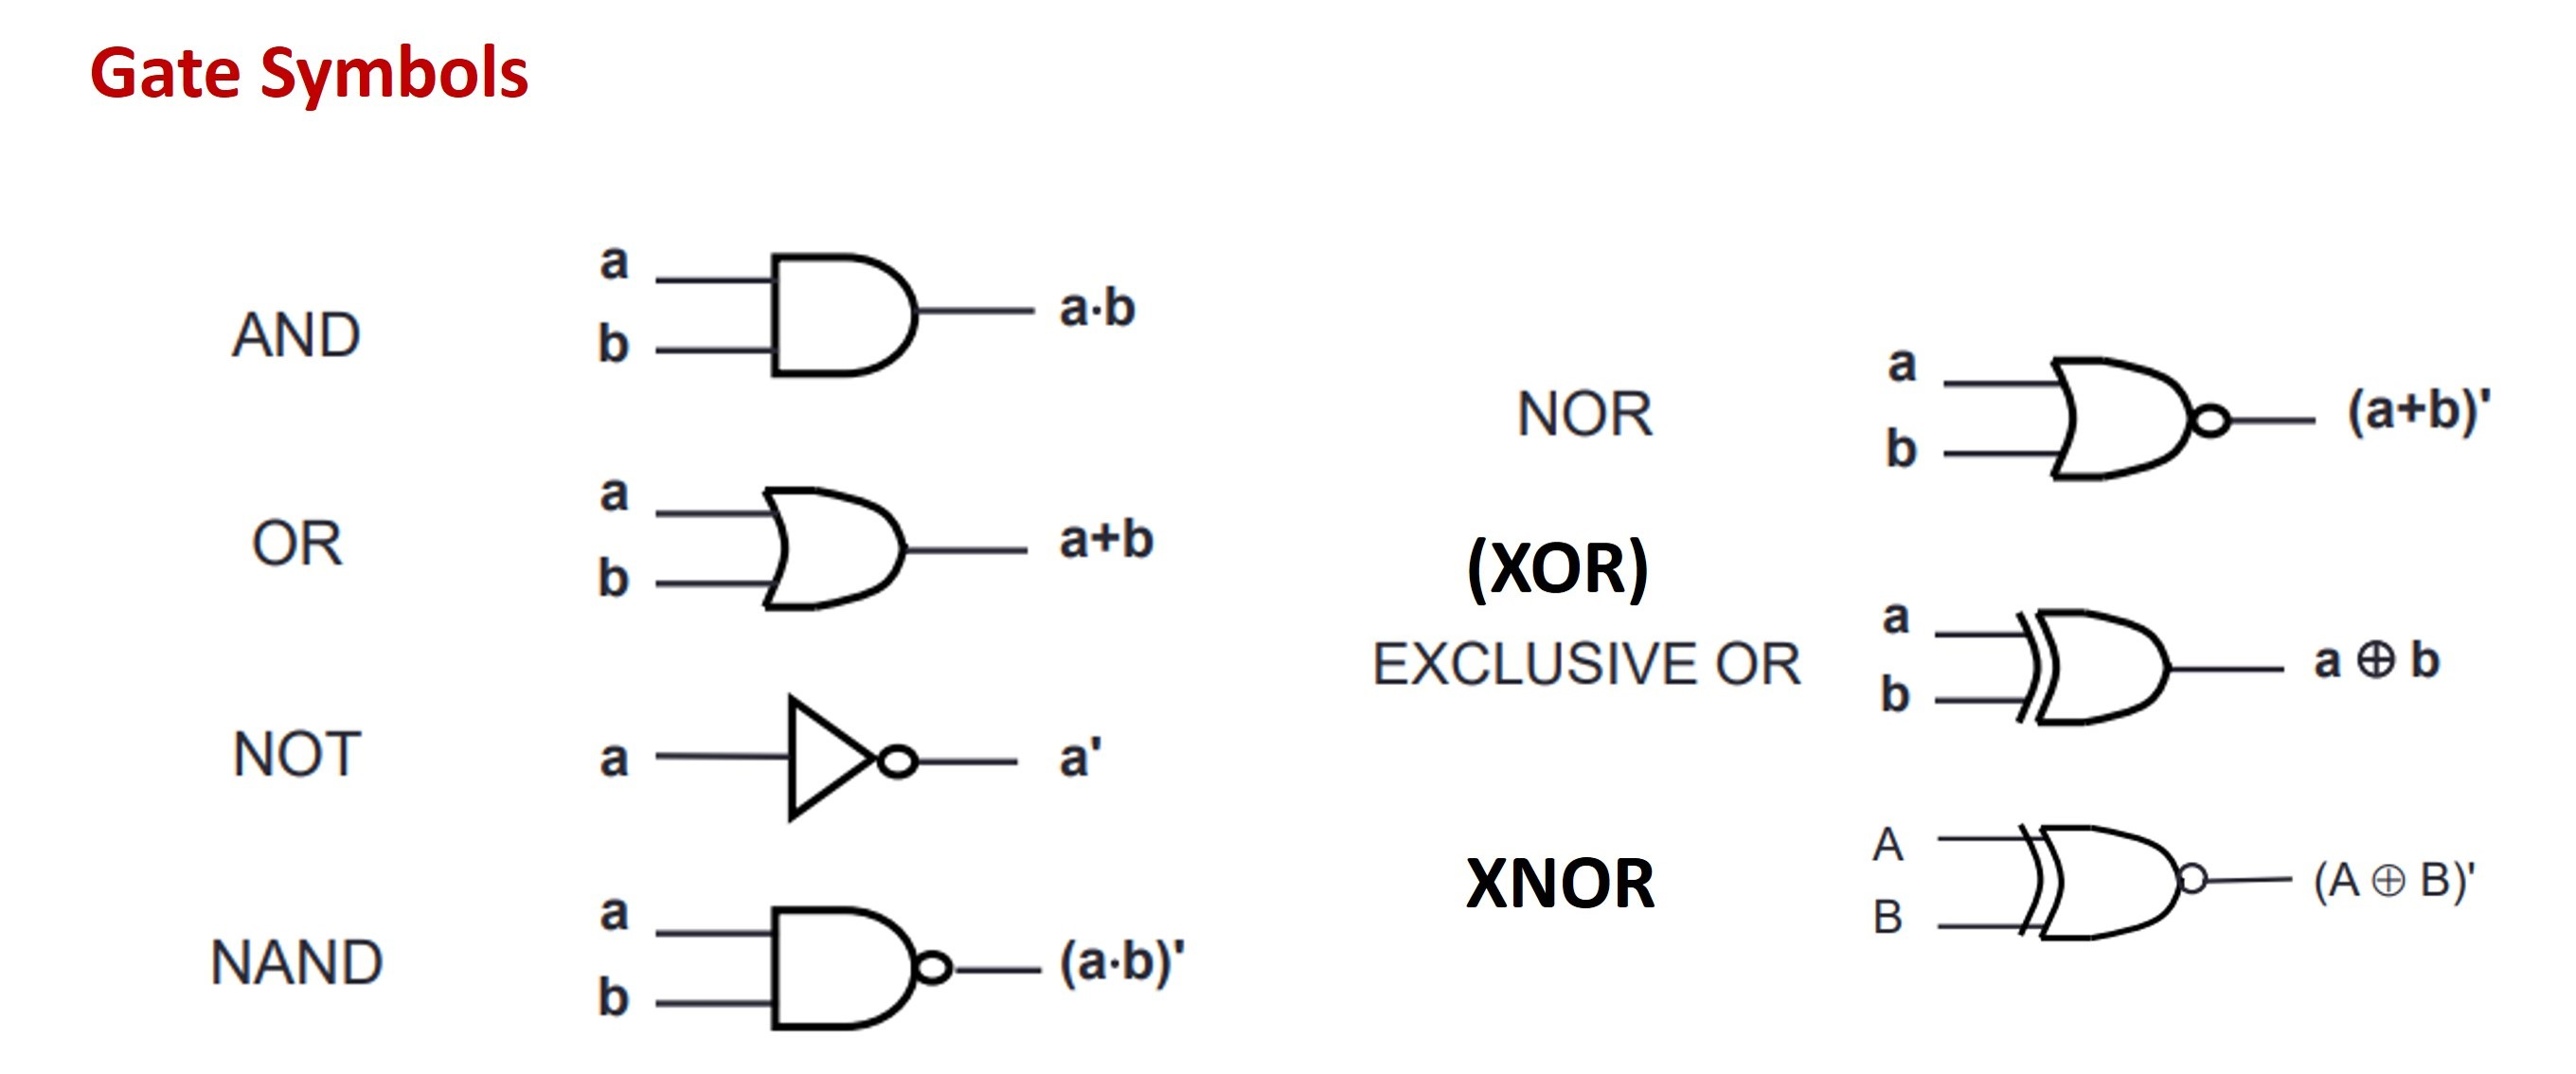
\includegraphics[width=1\linewidth]{logicgates1}}
\bigskip
\centerline{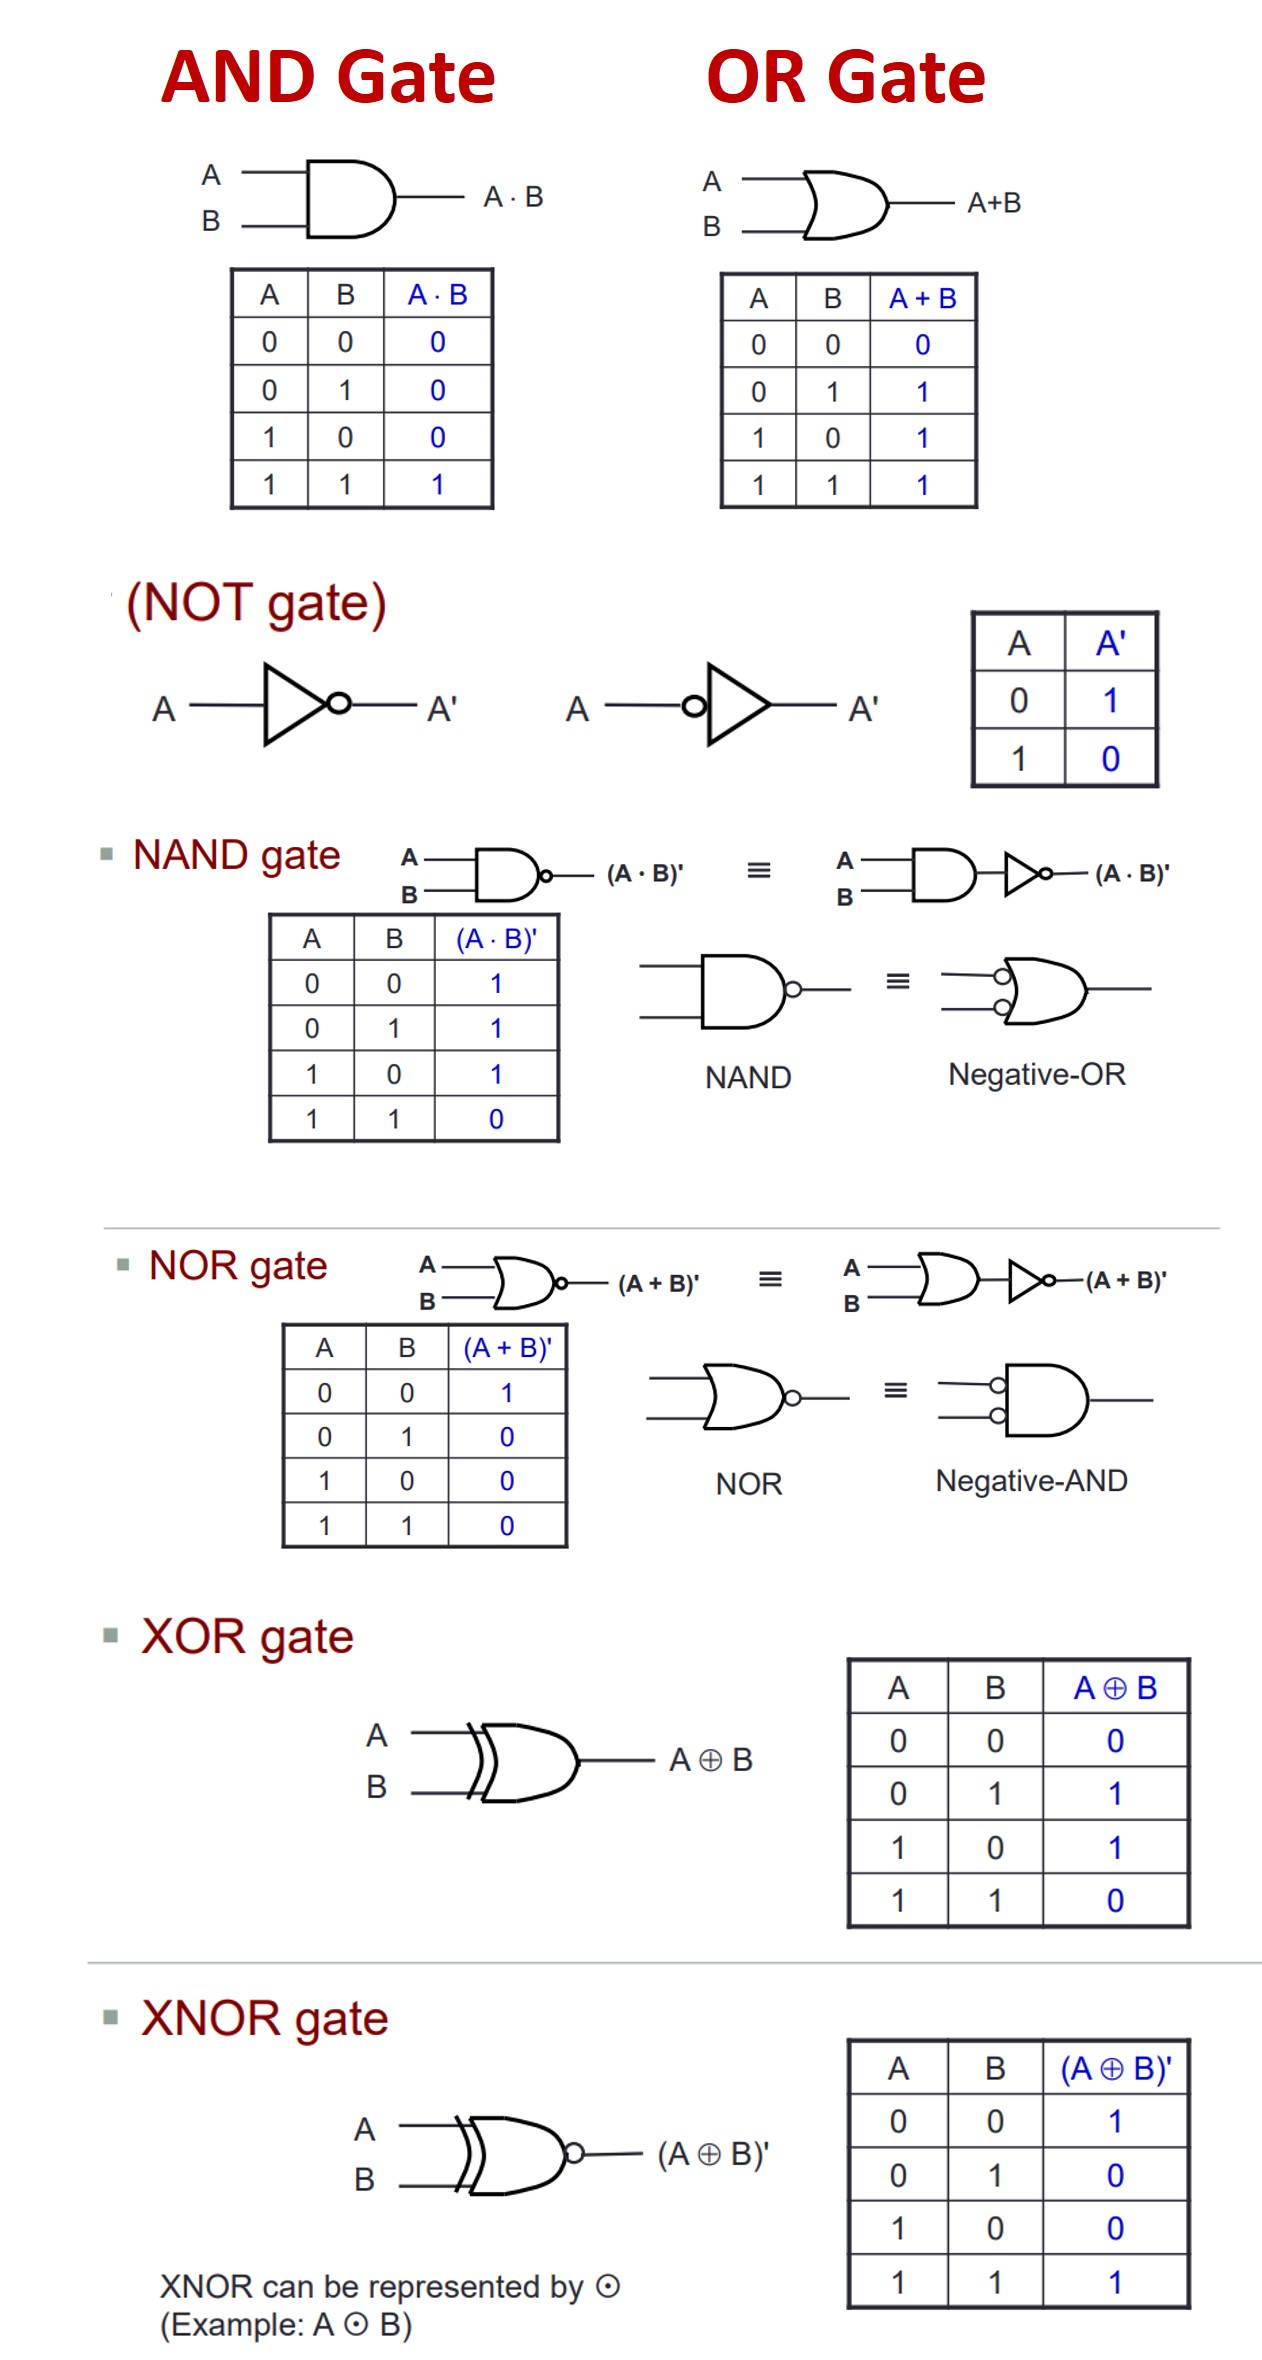
\includegraphics[width=0.9\linewidth]{logicgates2}}

\columnbreak

\subsubsection{NAND as Universal Gate (Complete Logic Set)}
\centerline{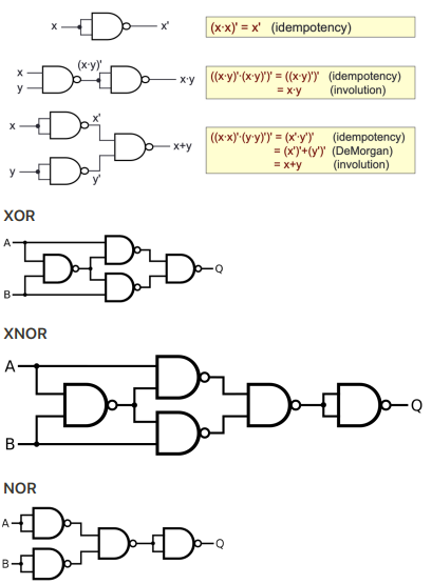
\includegraphics[width=0.75\linewidth]{NAND}}
\smallskip
\subsubsection{NOR as Universal Gate  (Complete Logic Set)}
\centerline{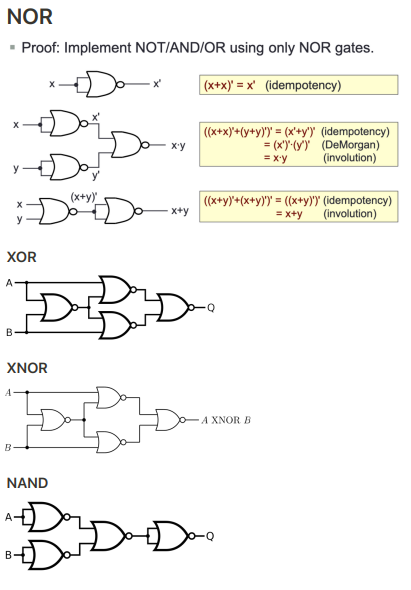
\includegraphics[width=0.75\linewidth]{NOR}}


\subsubsection{Gray Code}
\begin{itemize}
\item Only a \textbf{single bit change} from one code value to the next. 4 bit standard gray code:
\centerline{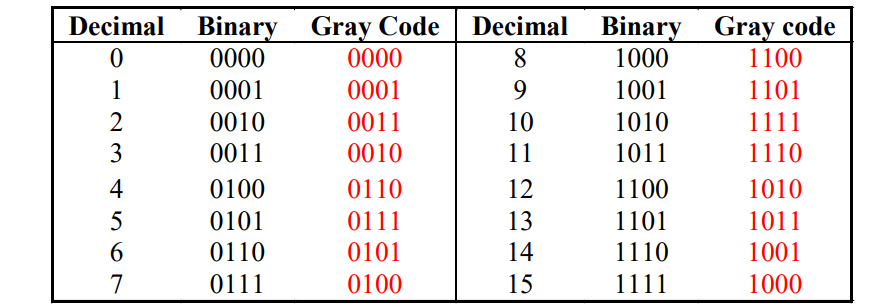
\includegraphics[width=0.9\linewidth]{graycode}}
\item not restricted to decimal digits: $n$ bits can have up to $2^n$ values.
\item aka reflected binary code. To generate gray code, reflect.
\item not unique - multiple possible Gray code sequences
\end{itemize}

\subsubsection{K Maps}
\begin{itemize}
\item Simplify (SOP) expressions, with fewest possible product terms and literals.
\item Based on \textbf{Unifying Theorem ($A + A' = 1$), complement law.}
\item Abstract form of Venn diagram, matrix of squares, each square represents a \textbf{minterm}.
\item Two adjacent squares represent minterms that differ by exactly one literal.
\centerline{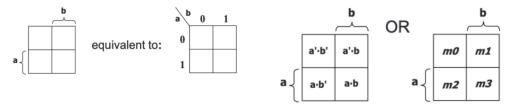
\includegraphics[width=1\linewidth]{kmap}}
\end{itemize}
\subsubsection{K Map for a function:}
\begin{itemize}
\item The K-map for a function is filled by putting: \\
◦ A \textbf{‘1’} in the square the corresponds to a \textbf{minterm} \\
◦ A ‘0’ otherwise
\item Each \textbf{valid grouping} of adjacent cells containing '1' corresponds to a
simpler product term. 
\item Group must have width/length (size) in \textbf{powers of 2}.
\item \textbf{larger group} = fewer literals in result product term
\item \textbf{fewer groups} = fewer product terms in final SOP exp.
\item Group maximum cells, and select fewest groups.
\end{itemize}


\vfill \null
\columnbreak

\section{K-Maps}
\subsubsection{3-Variable}
\centerline{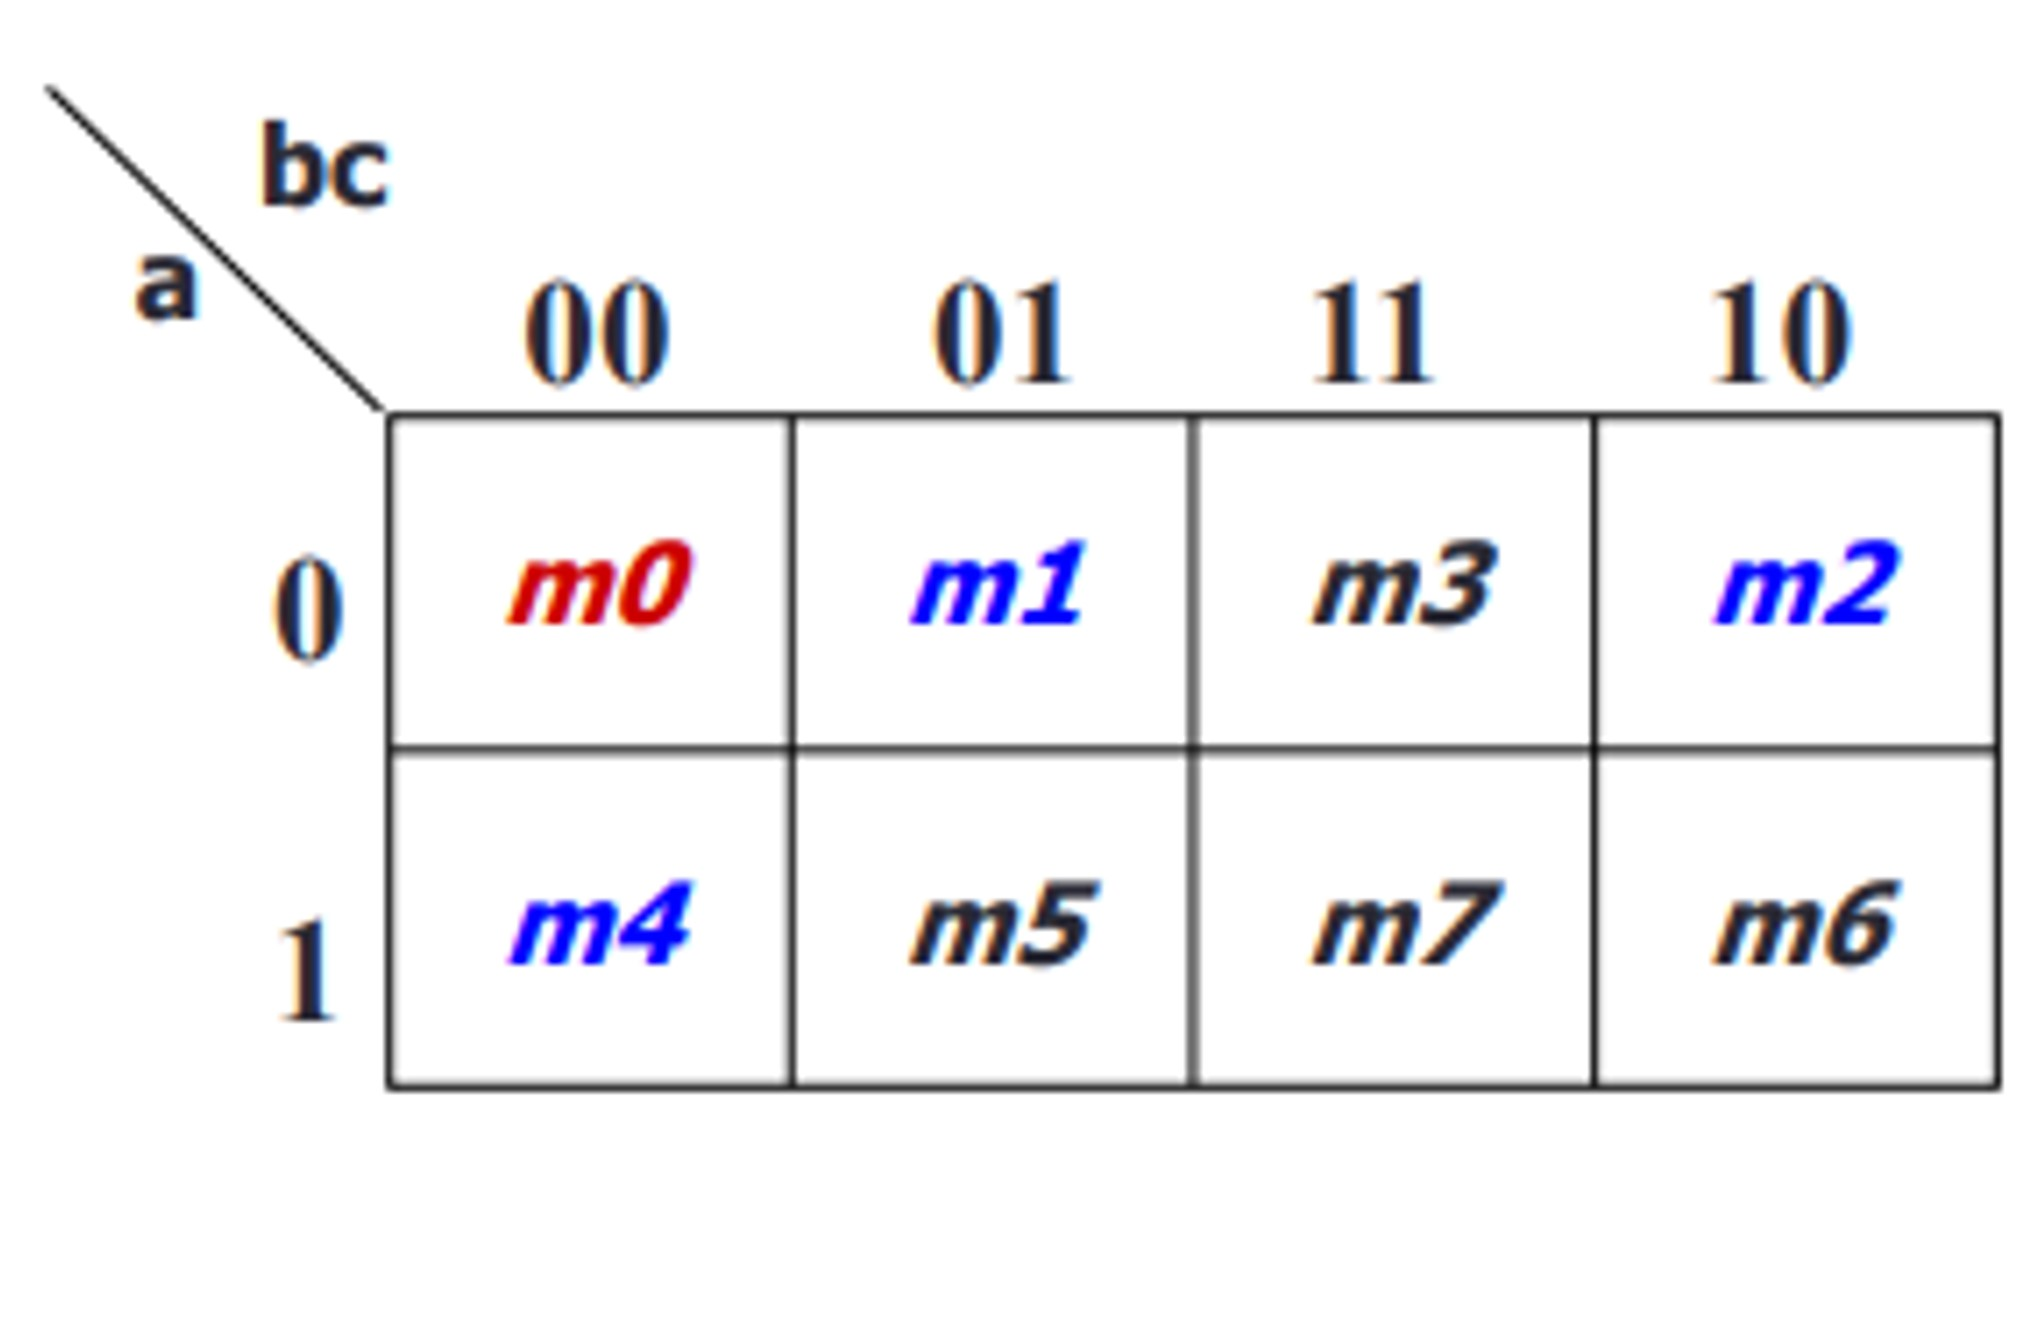
\includegraphics[width=0.7\linewidth]{3variable}}

\subsubsection{4-Variable}
\centerline{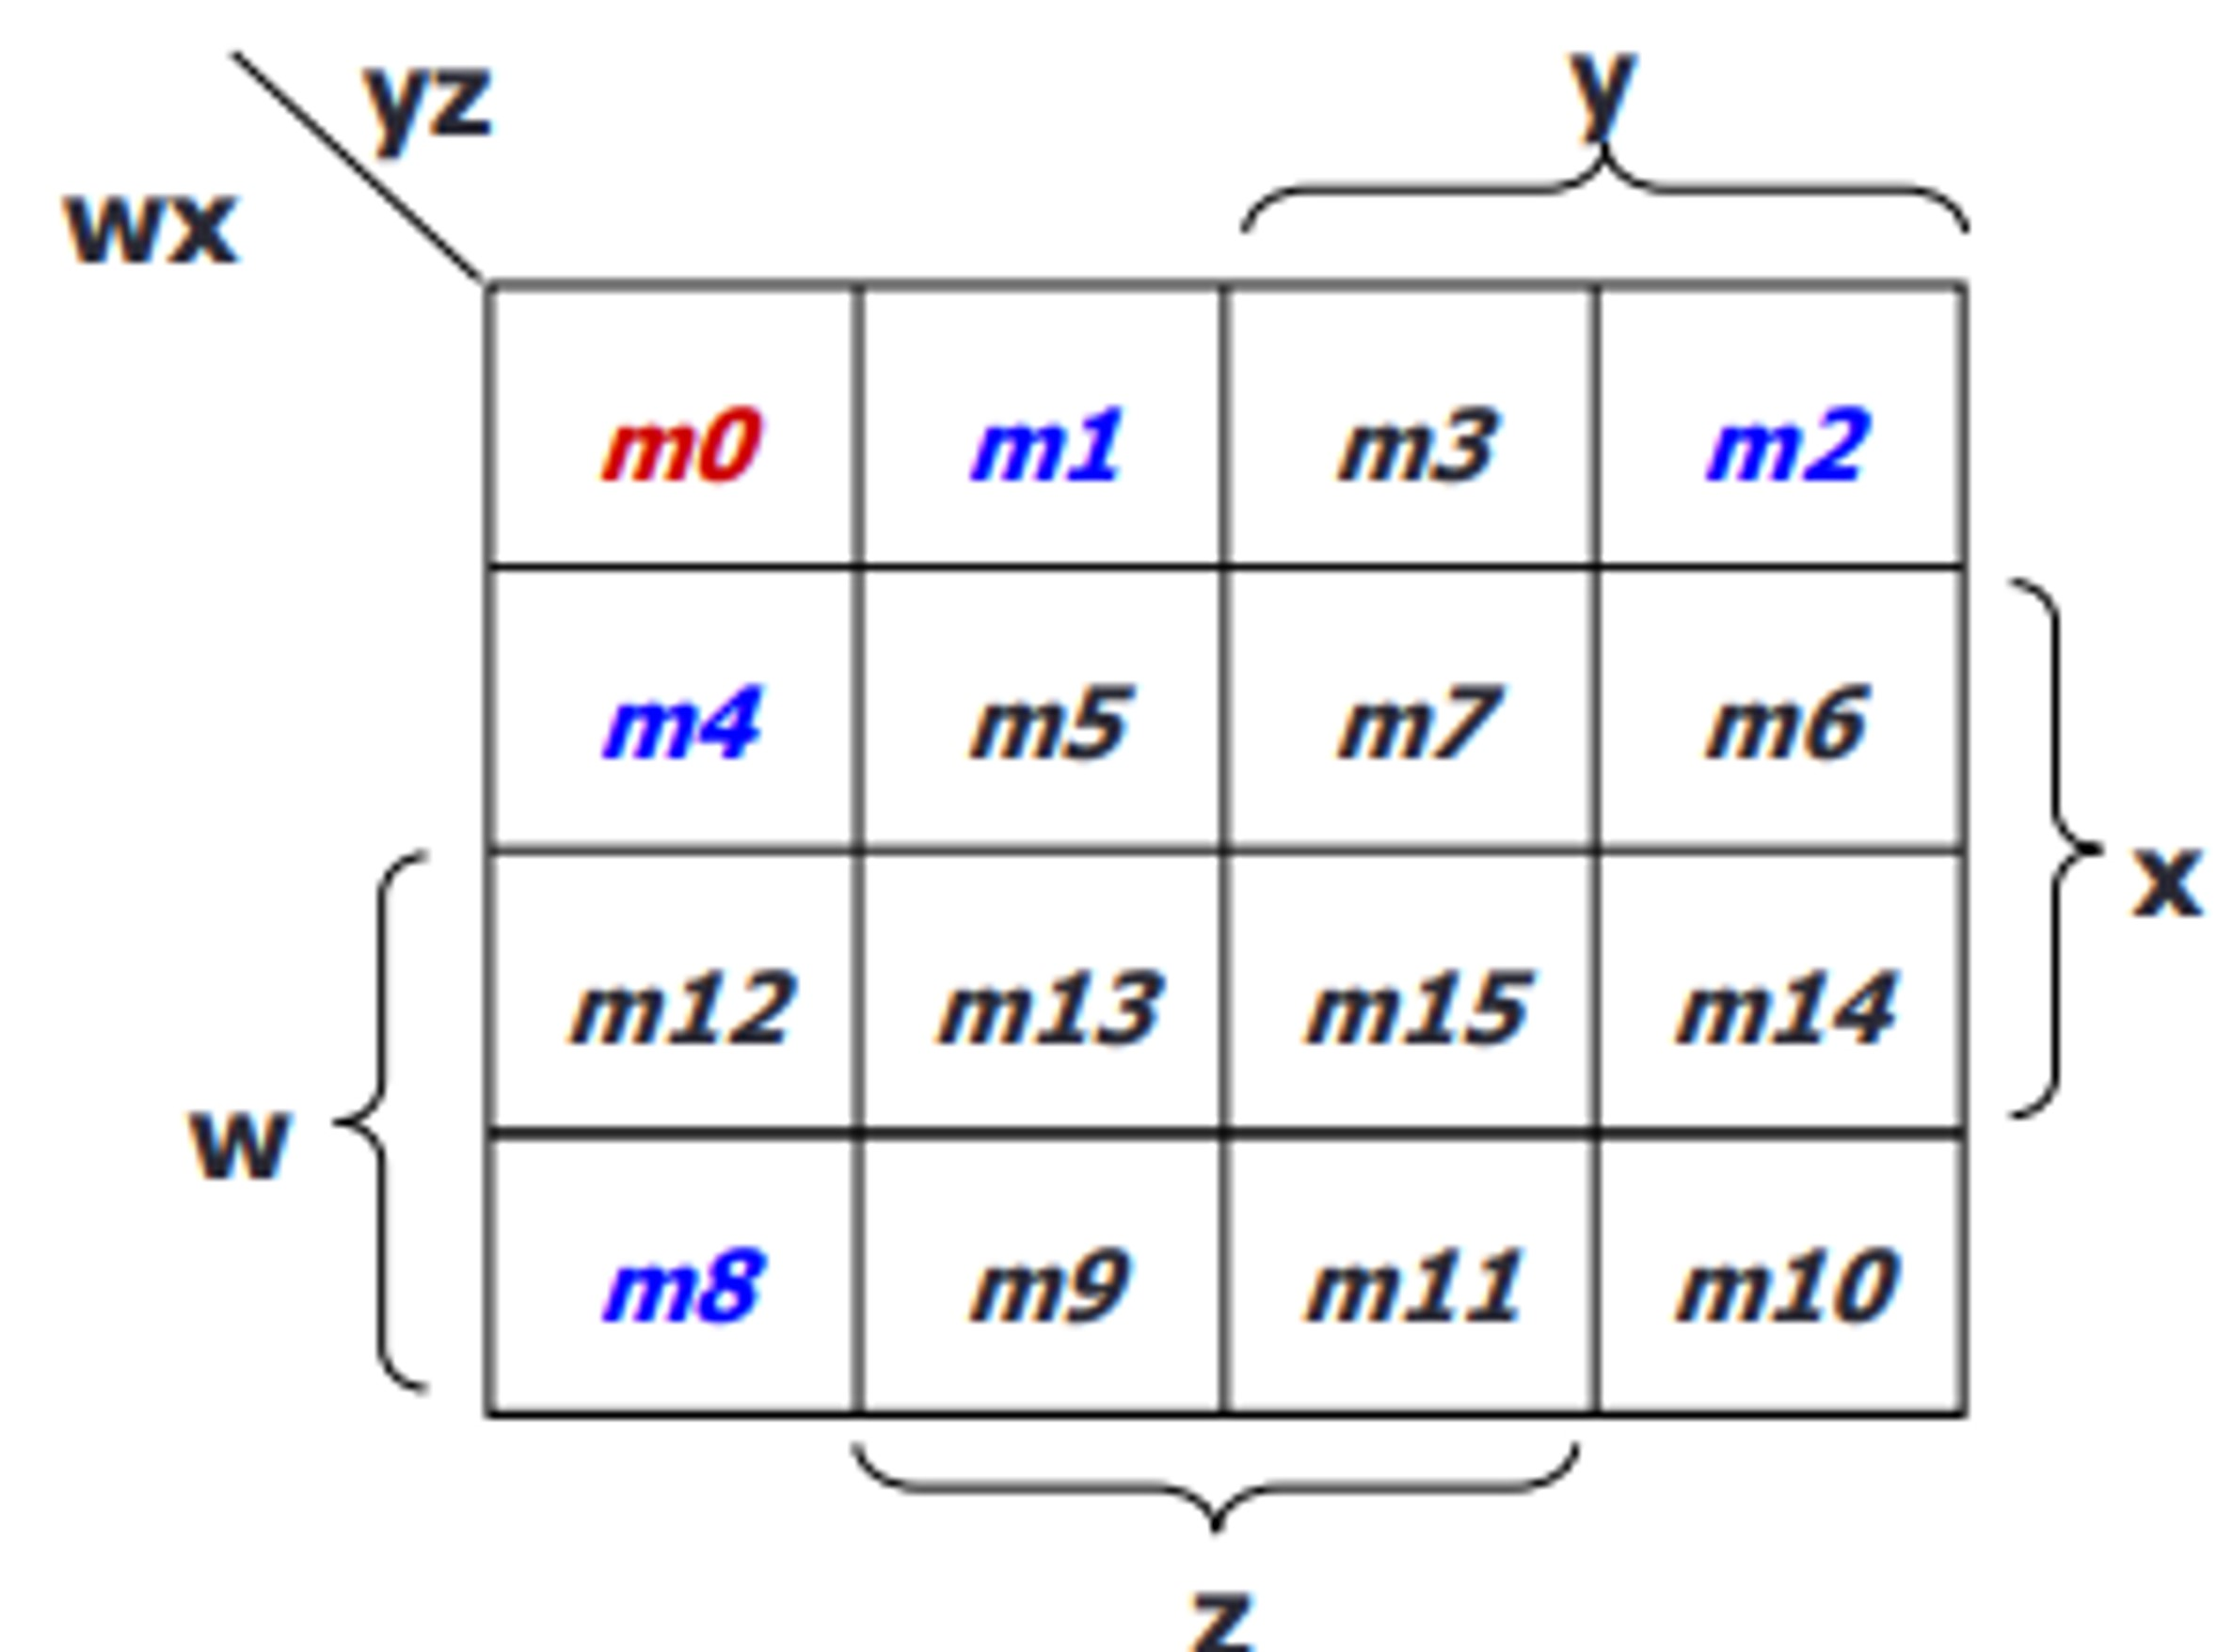
\includegraphics[width=0.8\linewidth]{4variable}}

\subsubsection{5-Variable}
\centerline{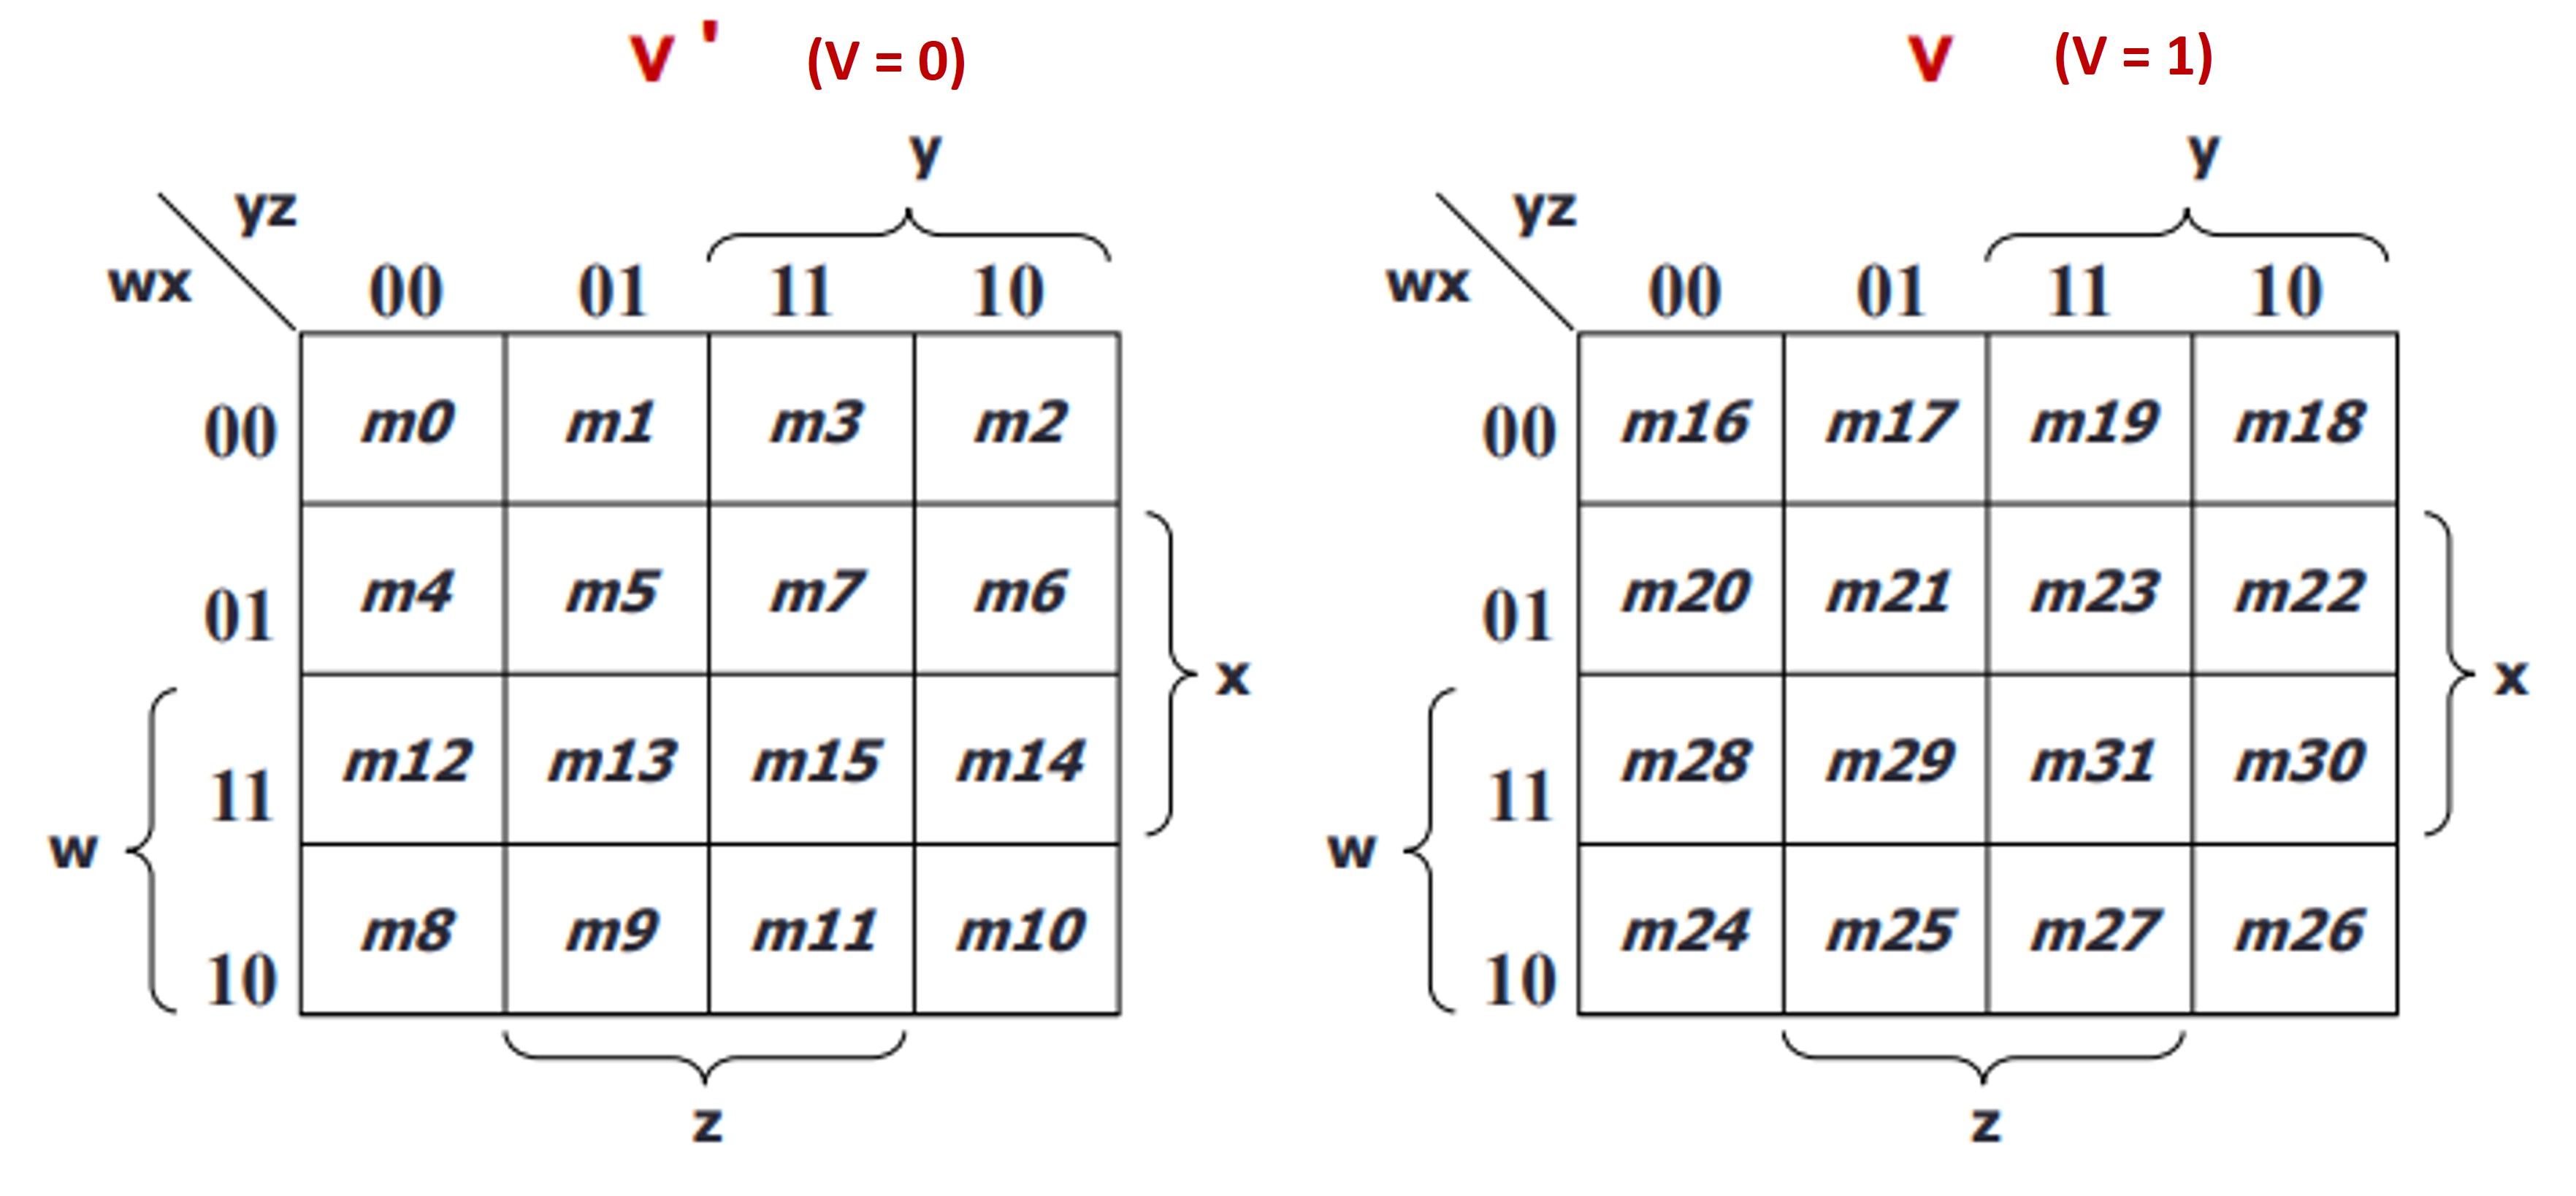
\includegraphics[width=1\linewidth]{5variable}}

\subsubsection{Valid Groupings}
\centerline{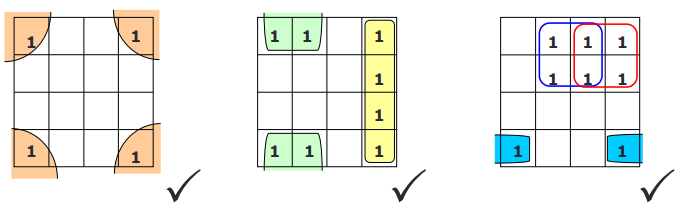
\includegraphics[width=1\linewidth]{validgroup}}

\subsubsection{6-Variable}
\centerline{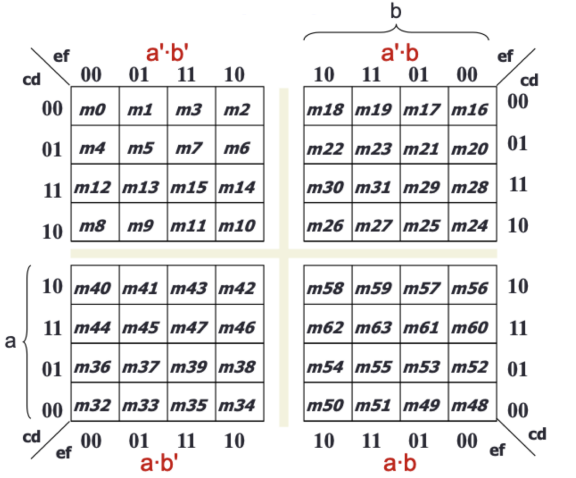
\includegraphics[width=0.9\linewidth]{6variable}}


\subsubsection{Using a K-map}
\begin{itemize}
\item K-map of function easily filled in when function in sum-of-minterms form. 
\item If not in sum-of-minterms, convert into sum-of-products (SOP) form, expand SOP expr into sum-of-minterms, or fill directly based on SOP.
\end{itemize}

\subsubsection{(E)PIs}
\begin{itemize}
\item \textbf{implicant}: product term that could be used to cover minterms of the function.
\item \textbf{prime implicant}: a product term obtained by combining the maximum possible number of minterms from adjacent squares in the map.
\item \textbf{essential prime implicant}: a prime implicant that includes at least one minterm that is not covered by any other prime implicant
\end{itemize}

\subsubsection{K-maps to find POS}
\begin{itemize}
\item shortcut: group maxterms (0s) of given function
\item long way: 1. convert K-map of F to K-map of F' (by flipping 0/1s), 2. get SOP of F' POS=(SOP)'.
\end{itemize}

\subsubsection{Don't-Care Conditions}
• denoted $d$, e.g.: $F(A, B, C) = \sum m(3, 5, 6) + \sum d(0, 7)$



\section{14. Combinational Circuits}
\subsubsection{Combinational Circuits}
\begin{itemize}
\item Two classes of logic circuits, combinational and sequential.
\centerline{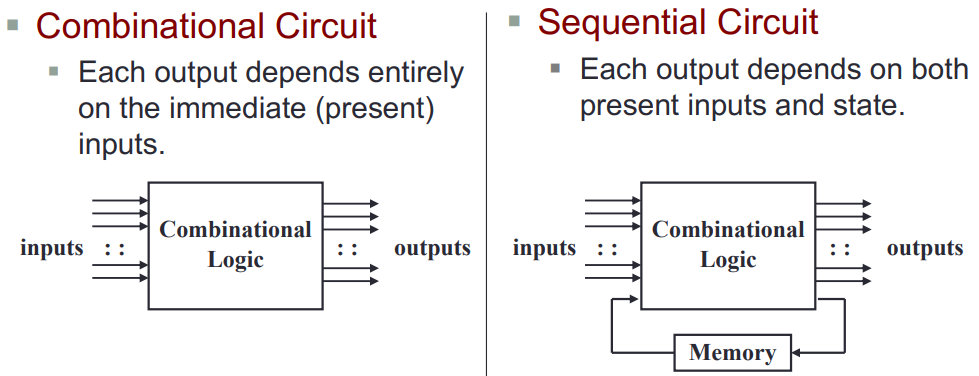
\includegraphics[width=0.8\linewidth]{logiccircuits}}
\item \textbf{Function analysis of combinational circuit (CC)}: Label inputs and outputs, obtain functions of intermediate points and draw the truth table. Deduce functionality.
\item \textbf{CC design methods}: gate-level (with logic gates) and block-level (with functional blocks, e.g. IC chip).
\item Goals: reduce cost, increase speed, design simplicity.
\end{itemize}

\subsubsection{Gate-Level (SSI: Small Scale Integration) Design}
\begin{itemize}
\item Design procedure: \\
1. State problem, label input output of circuit.\\
2. Draw truth table, obtain simplified boolean function. \\
3. Draw logic diagram.
\end{itemize}
\centerline{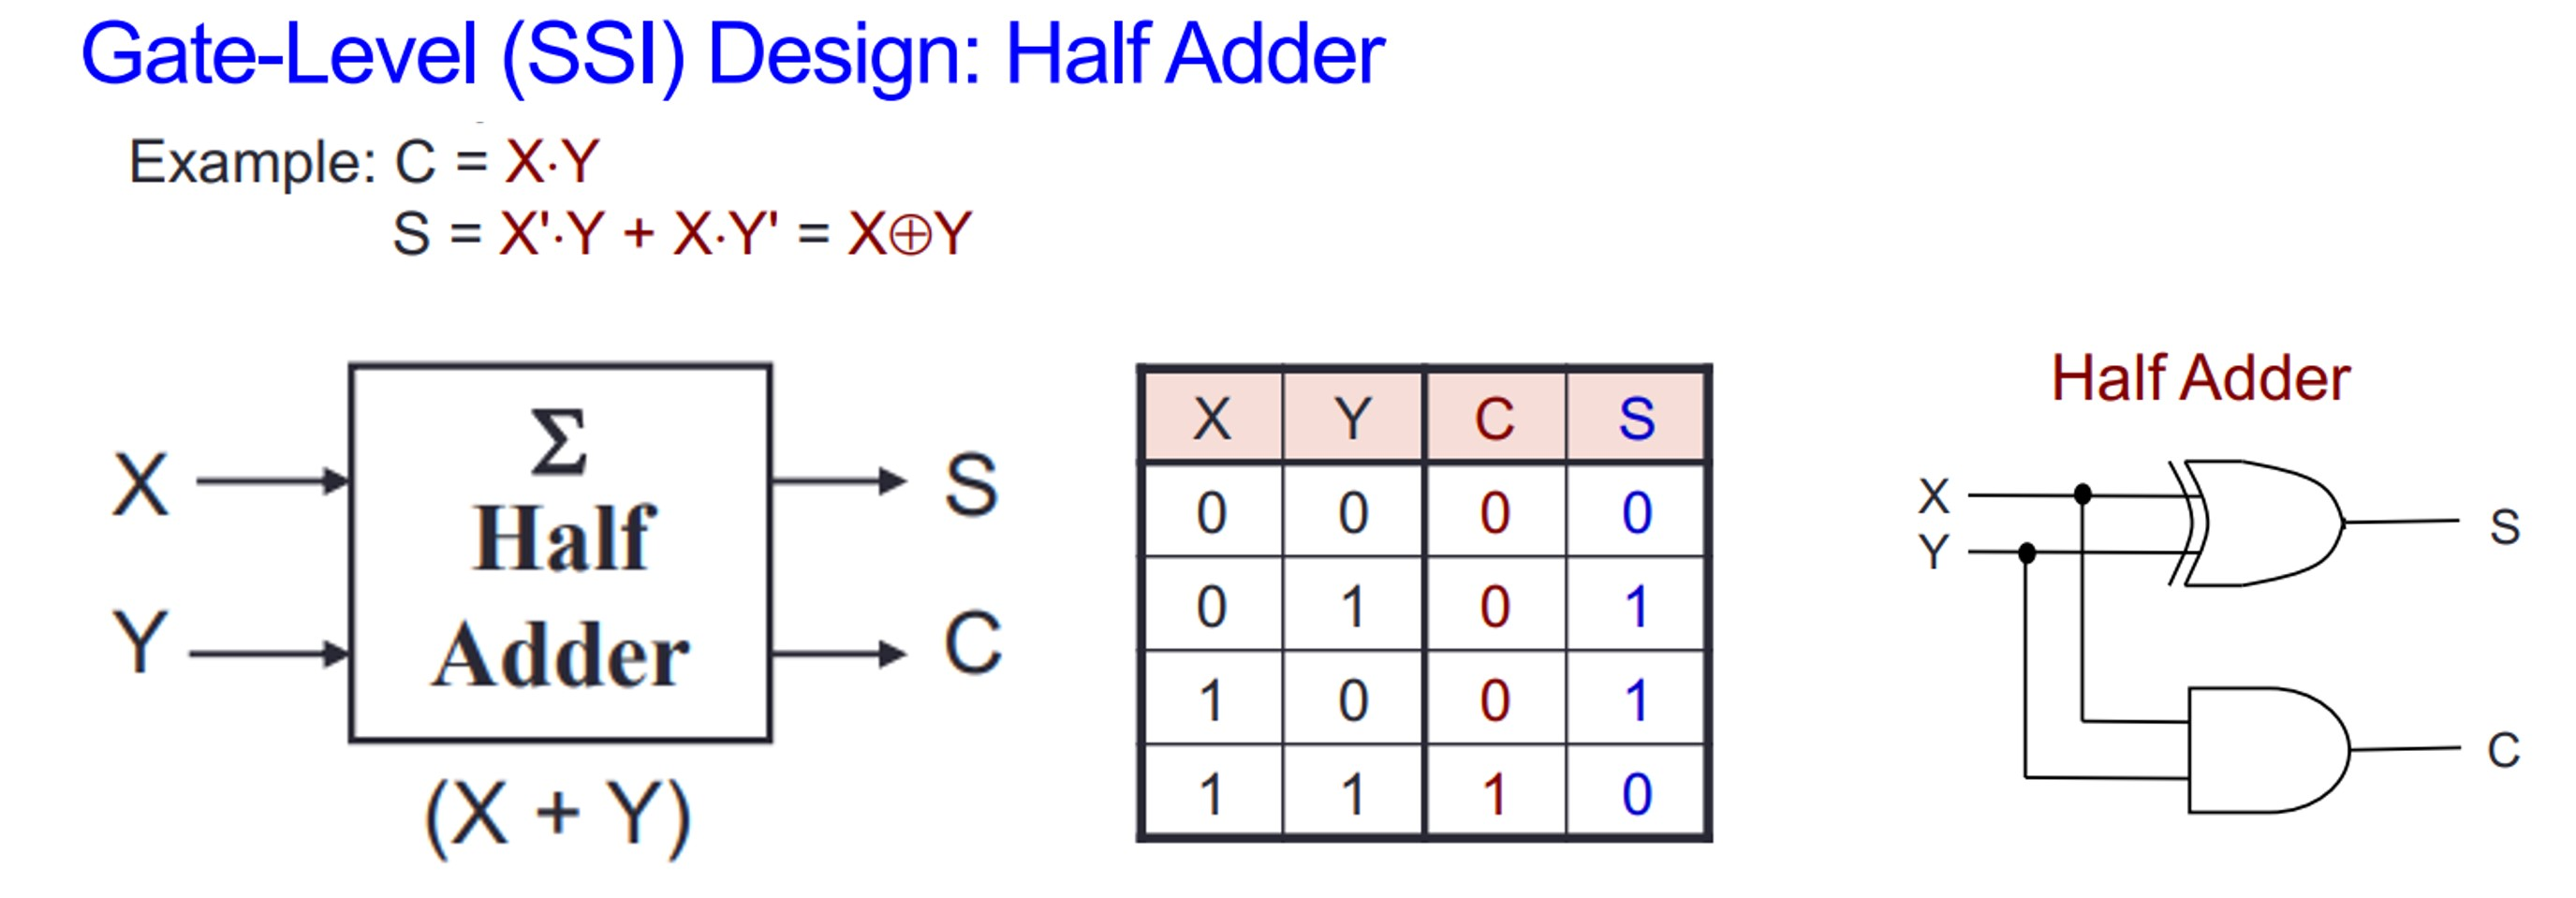
\includegraphics[width=1\linewidth]{buildha}}
\bigskip
\centerline{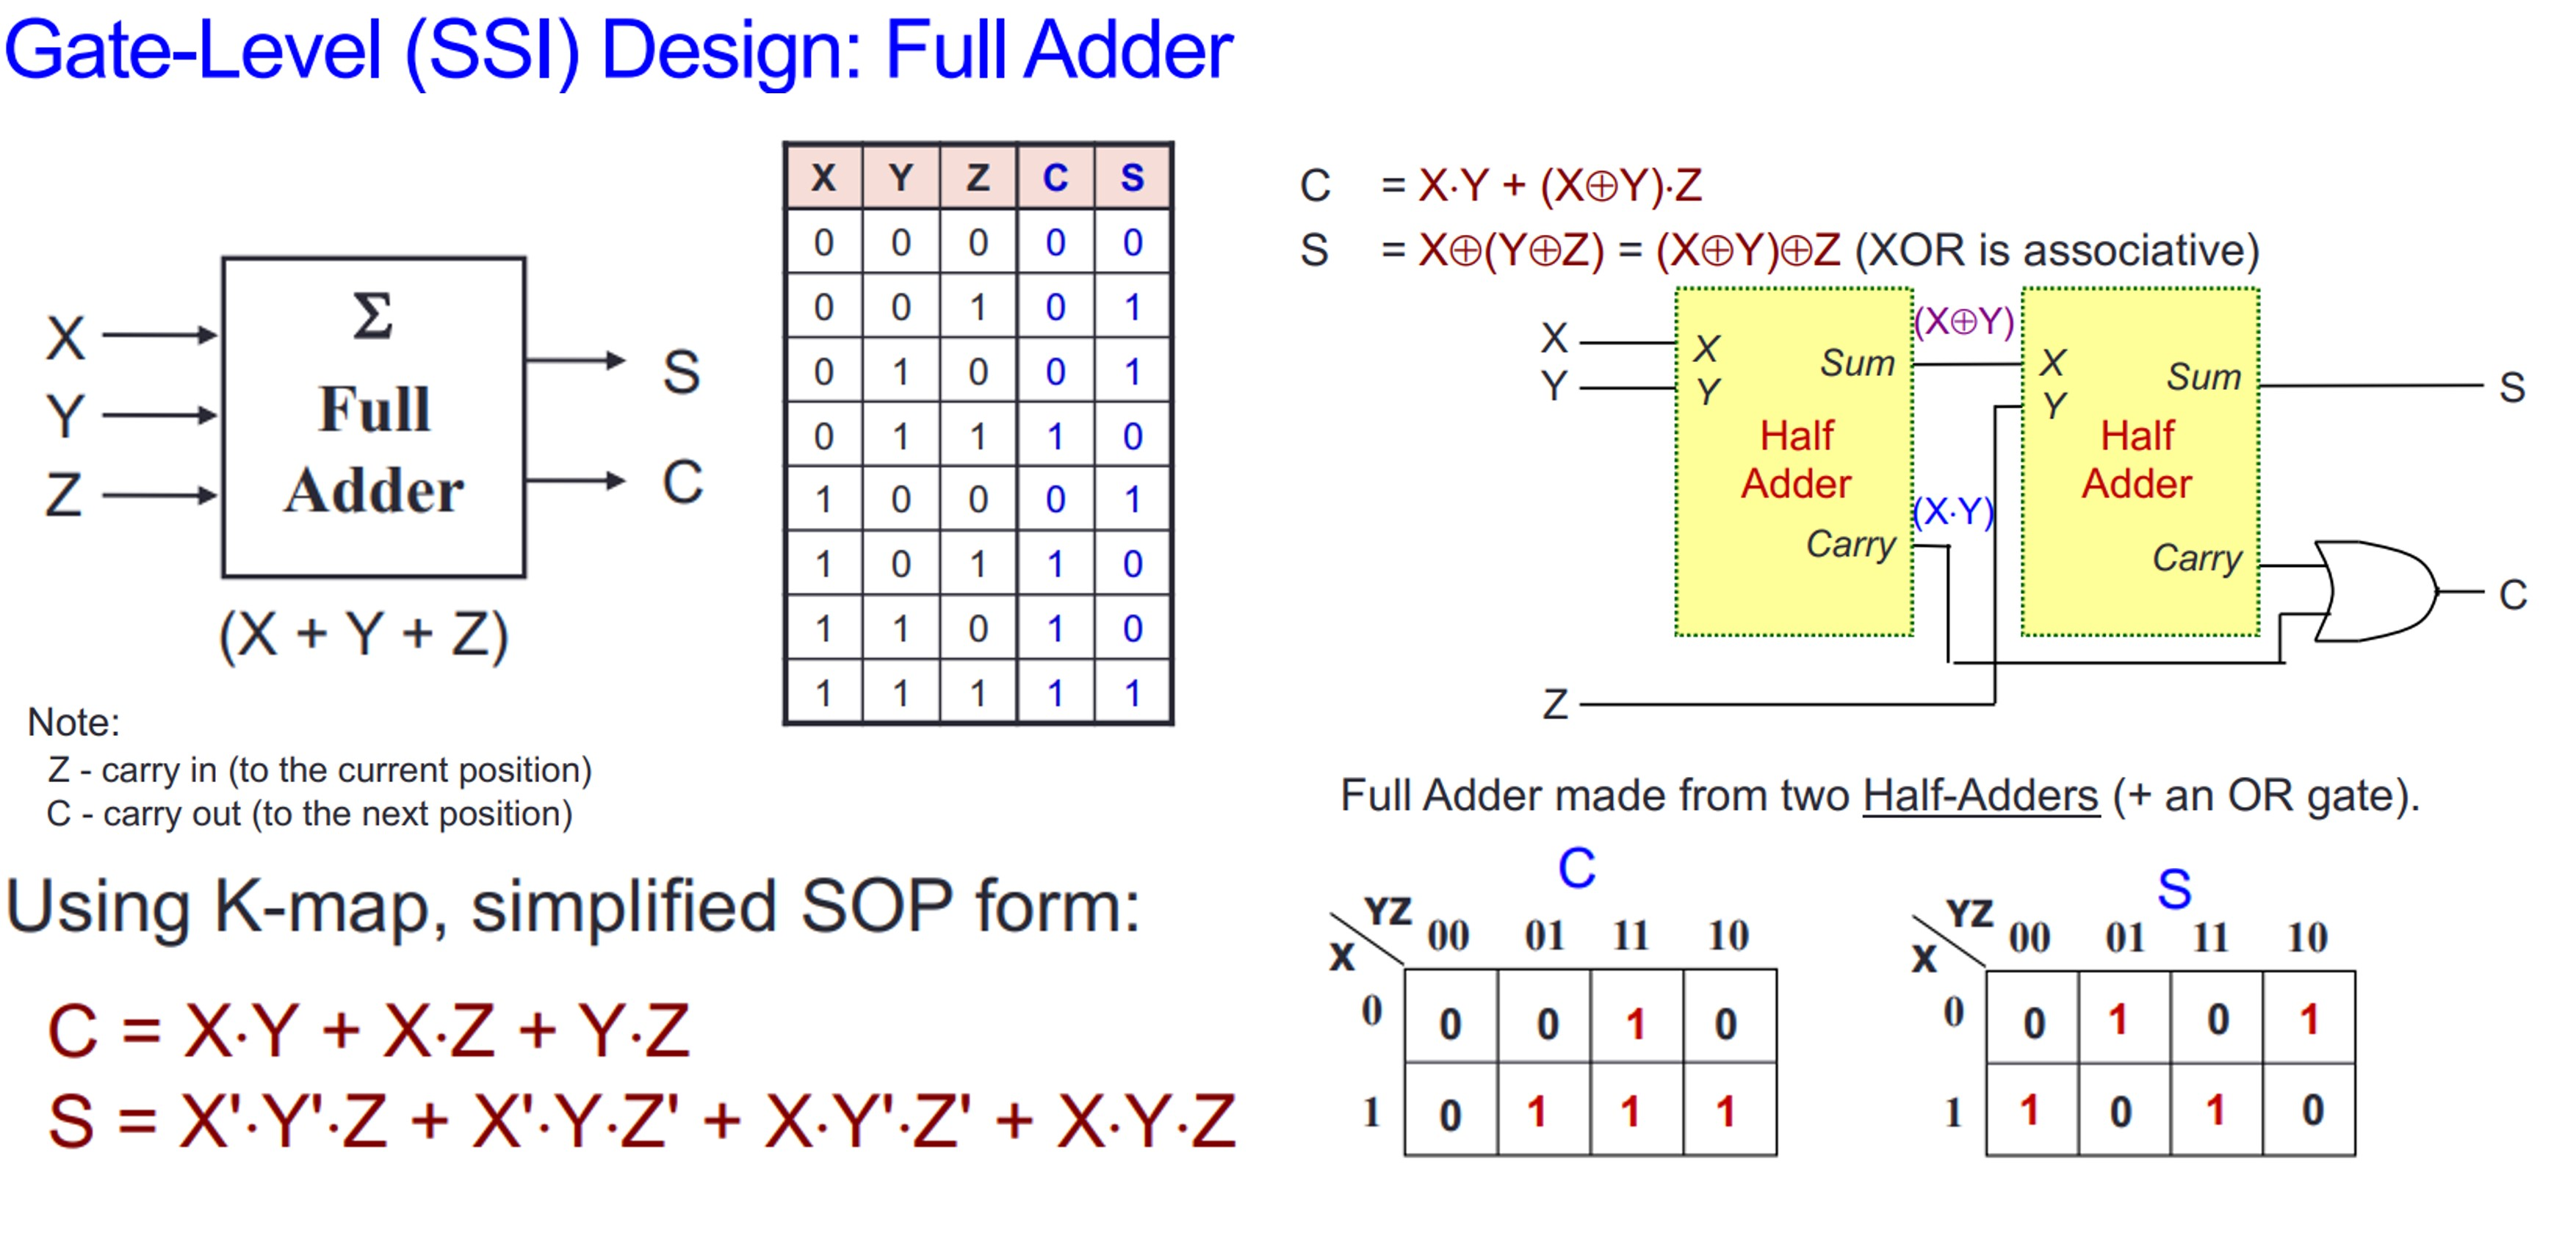
\includegraphics[width=1\linewidth]{buildfa}}

\subsubsection{Arithmetic Circuits Summary}
\begin{itemize}
\item \textbf{Block-Level Design} More complex circuits built using block-level method, rely on algorithm or formulae of circuit, 
decompose problem into solvable subproblems.
\end{itemize}
\centerline{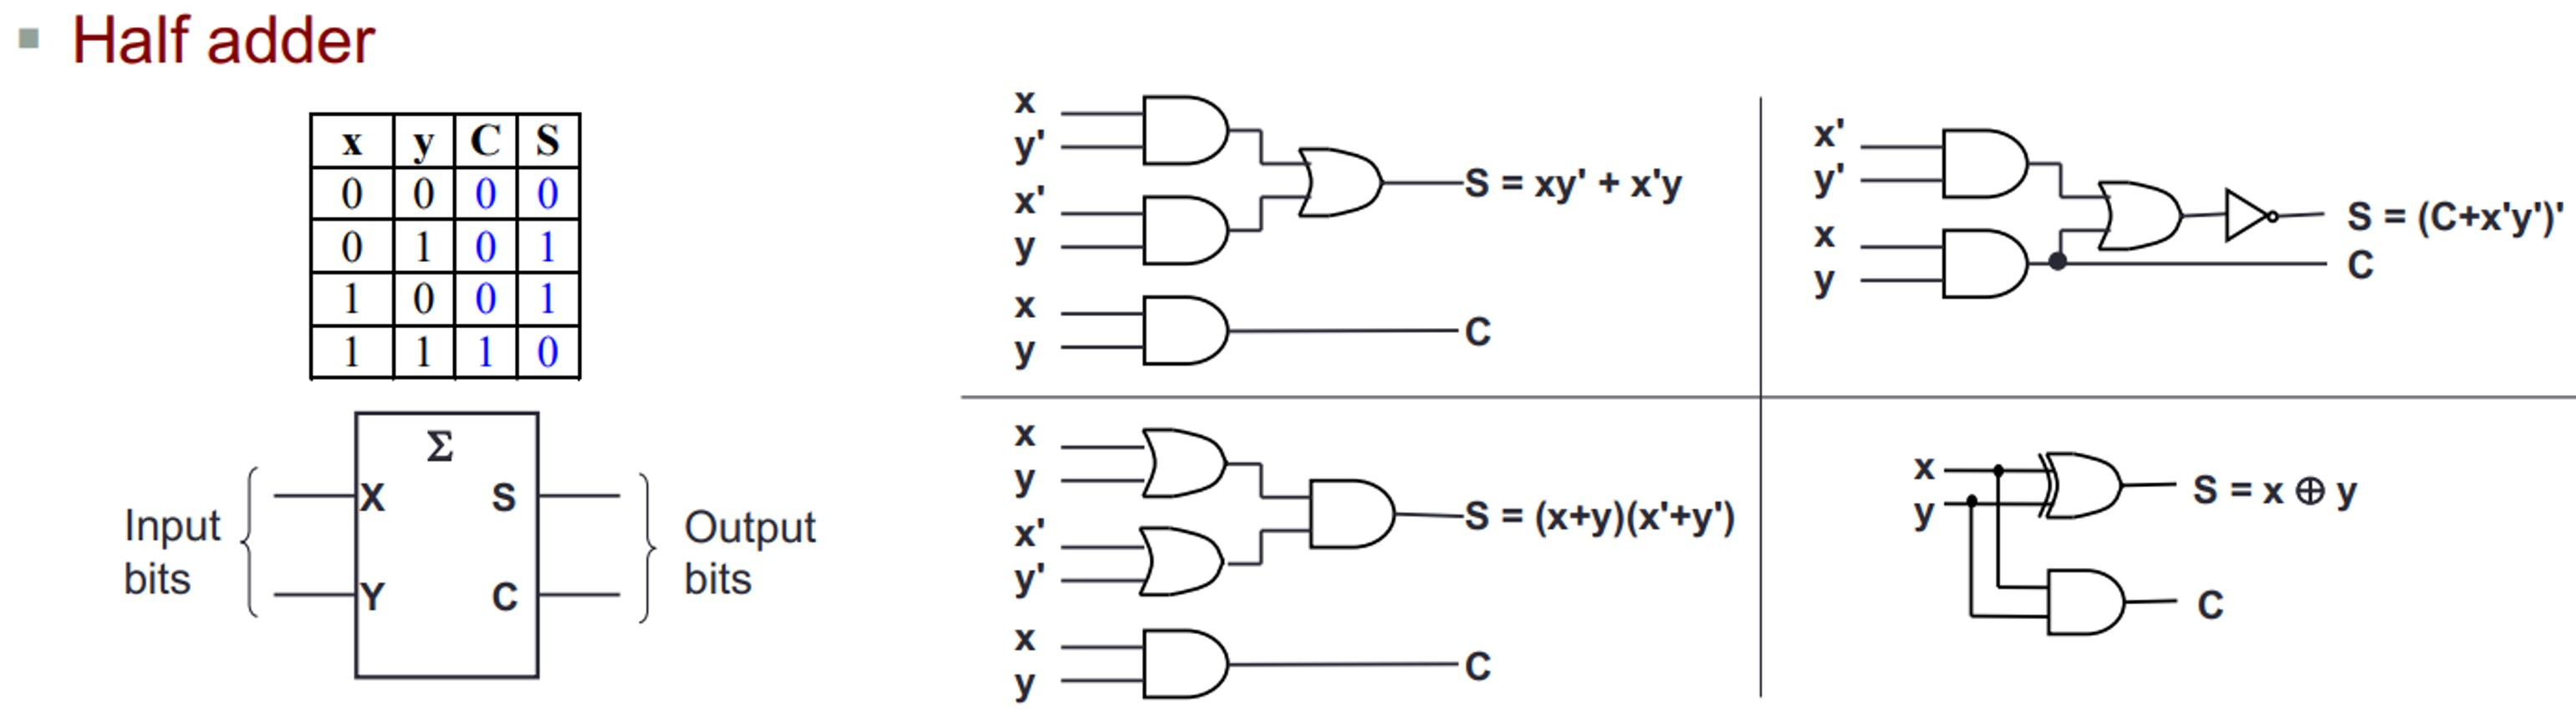
\includegraphics[width=1\linewidth]{ha}}
\bigskip
\centerline{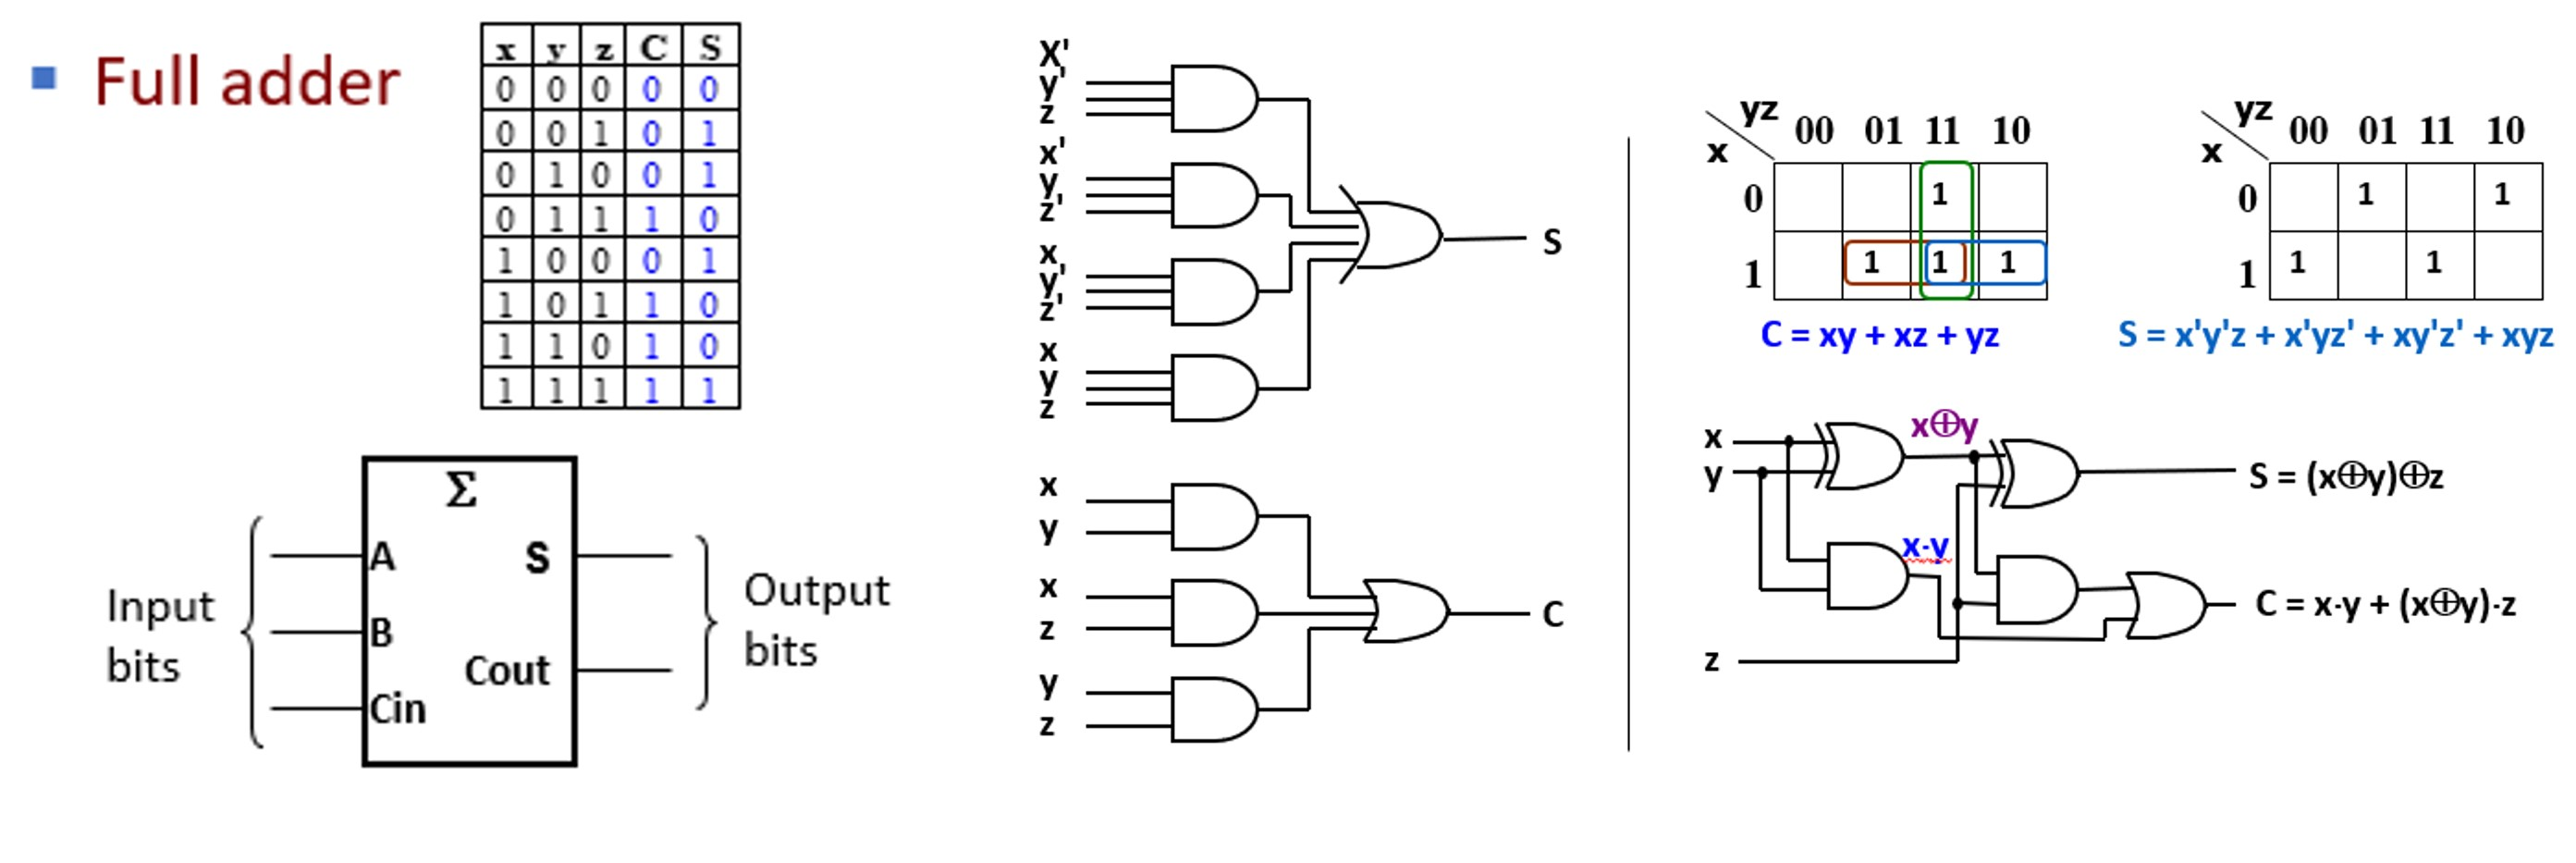
\includegraphics[width=1\linewidth]{fa}}
\bigskip
\centerline{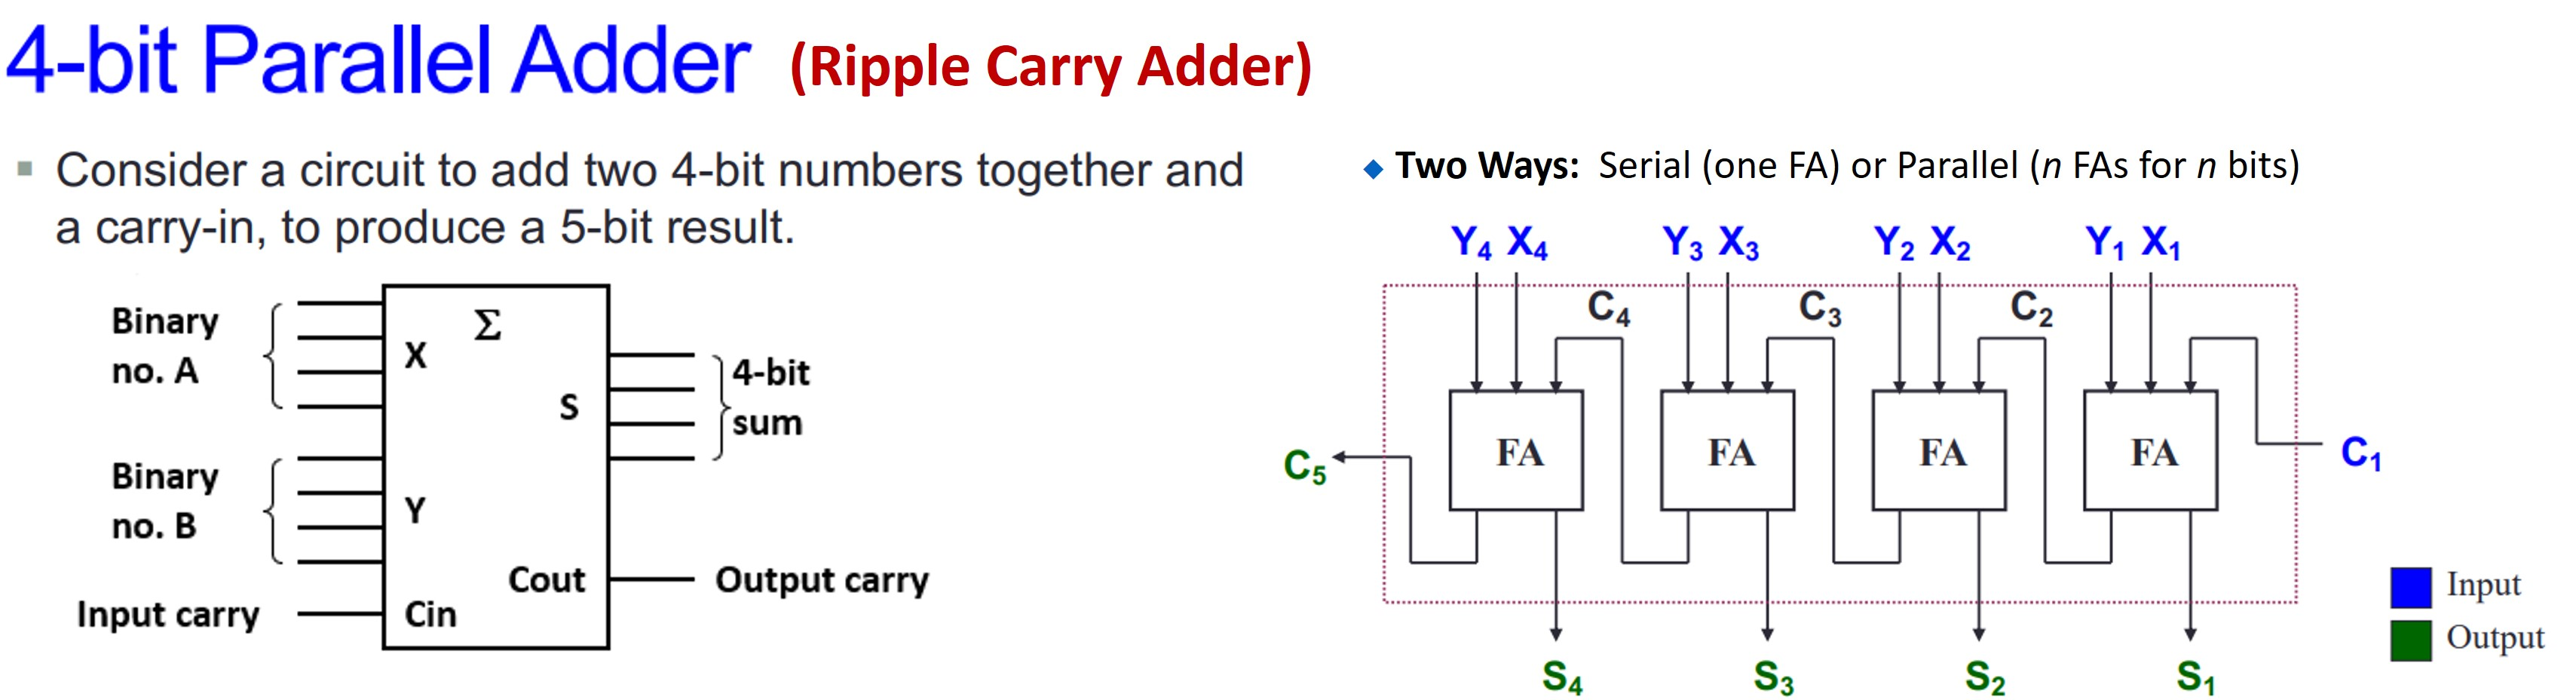
\includegraphics[width=1\linewidth]{4badder}}

\subsubsection{Circuit Delays}
\begin{itemize}
\item Given a \textbf{logic gate} with delay $t$. If inputs stable at times $t1, t2, …, tn,$ then earliest time in which 
output will be stable is: $max( t1, t2, …, tn ) + t$  \\ \medskip
\centerline{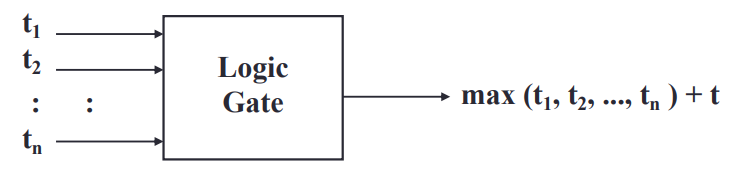
\includegraphics[width=0.8\linewidth]{circuitdelay}}
\item delay of a combinational circuit: repeat for all gates
\item E.g. n-bit parallel adder will have delay of: \\
$S_n = ( (n – 1) * 2 + 2 ) t $ \\
$C_{n+1} = ( (n – 1) * 2 + 3 ) t $ \\
\textbf{max delay} = $( (n – 1)* 2 + 3 ) t$
\end{itemize}


\columnbreak

\subsubsection{Block Diagrams}
\centerline{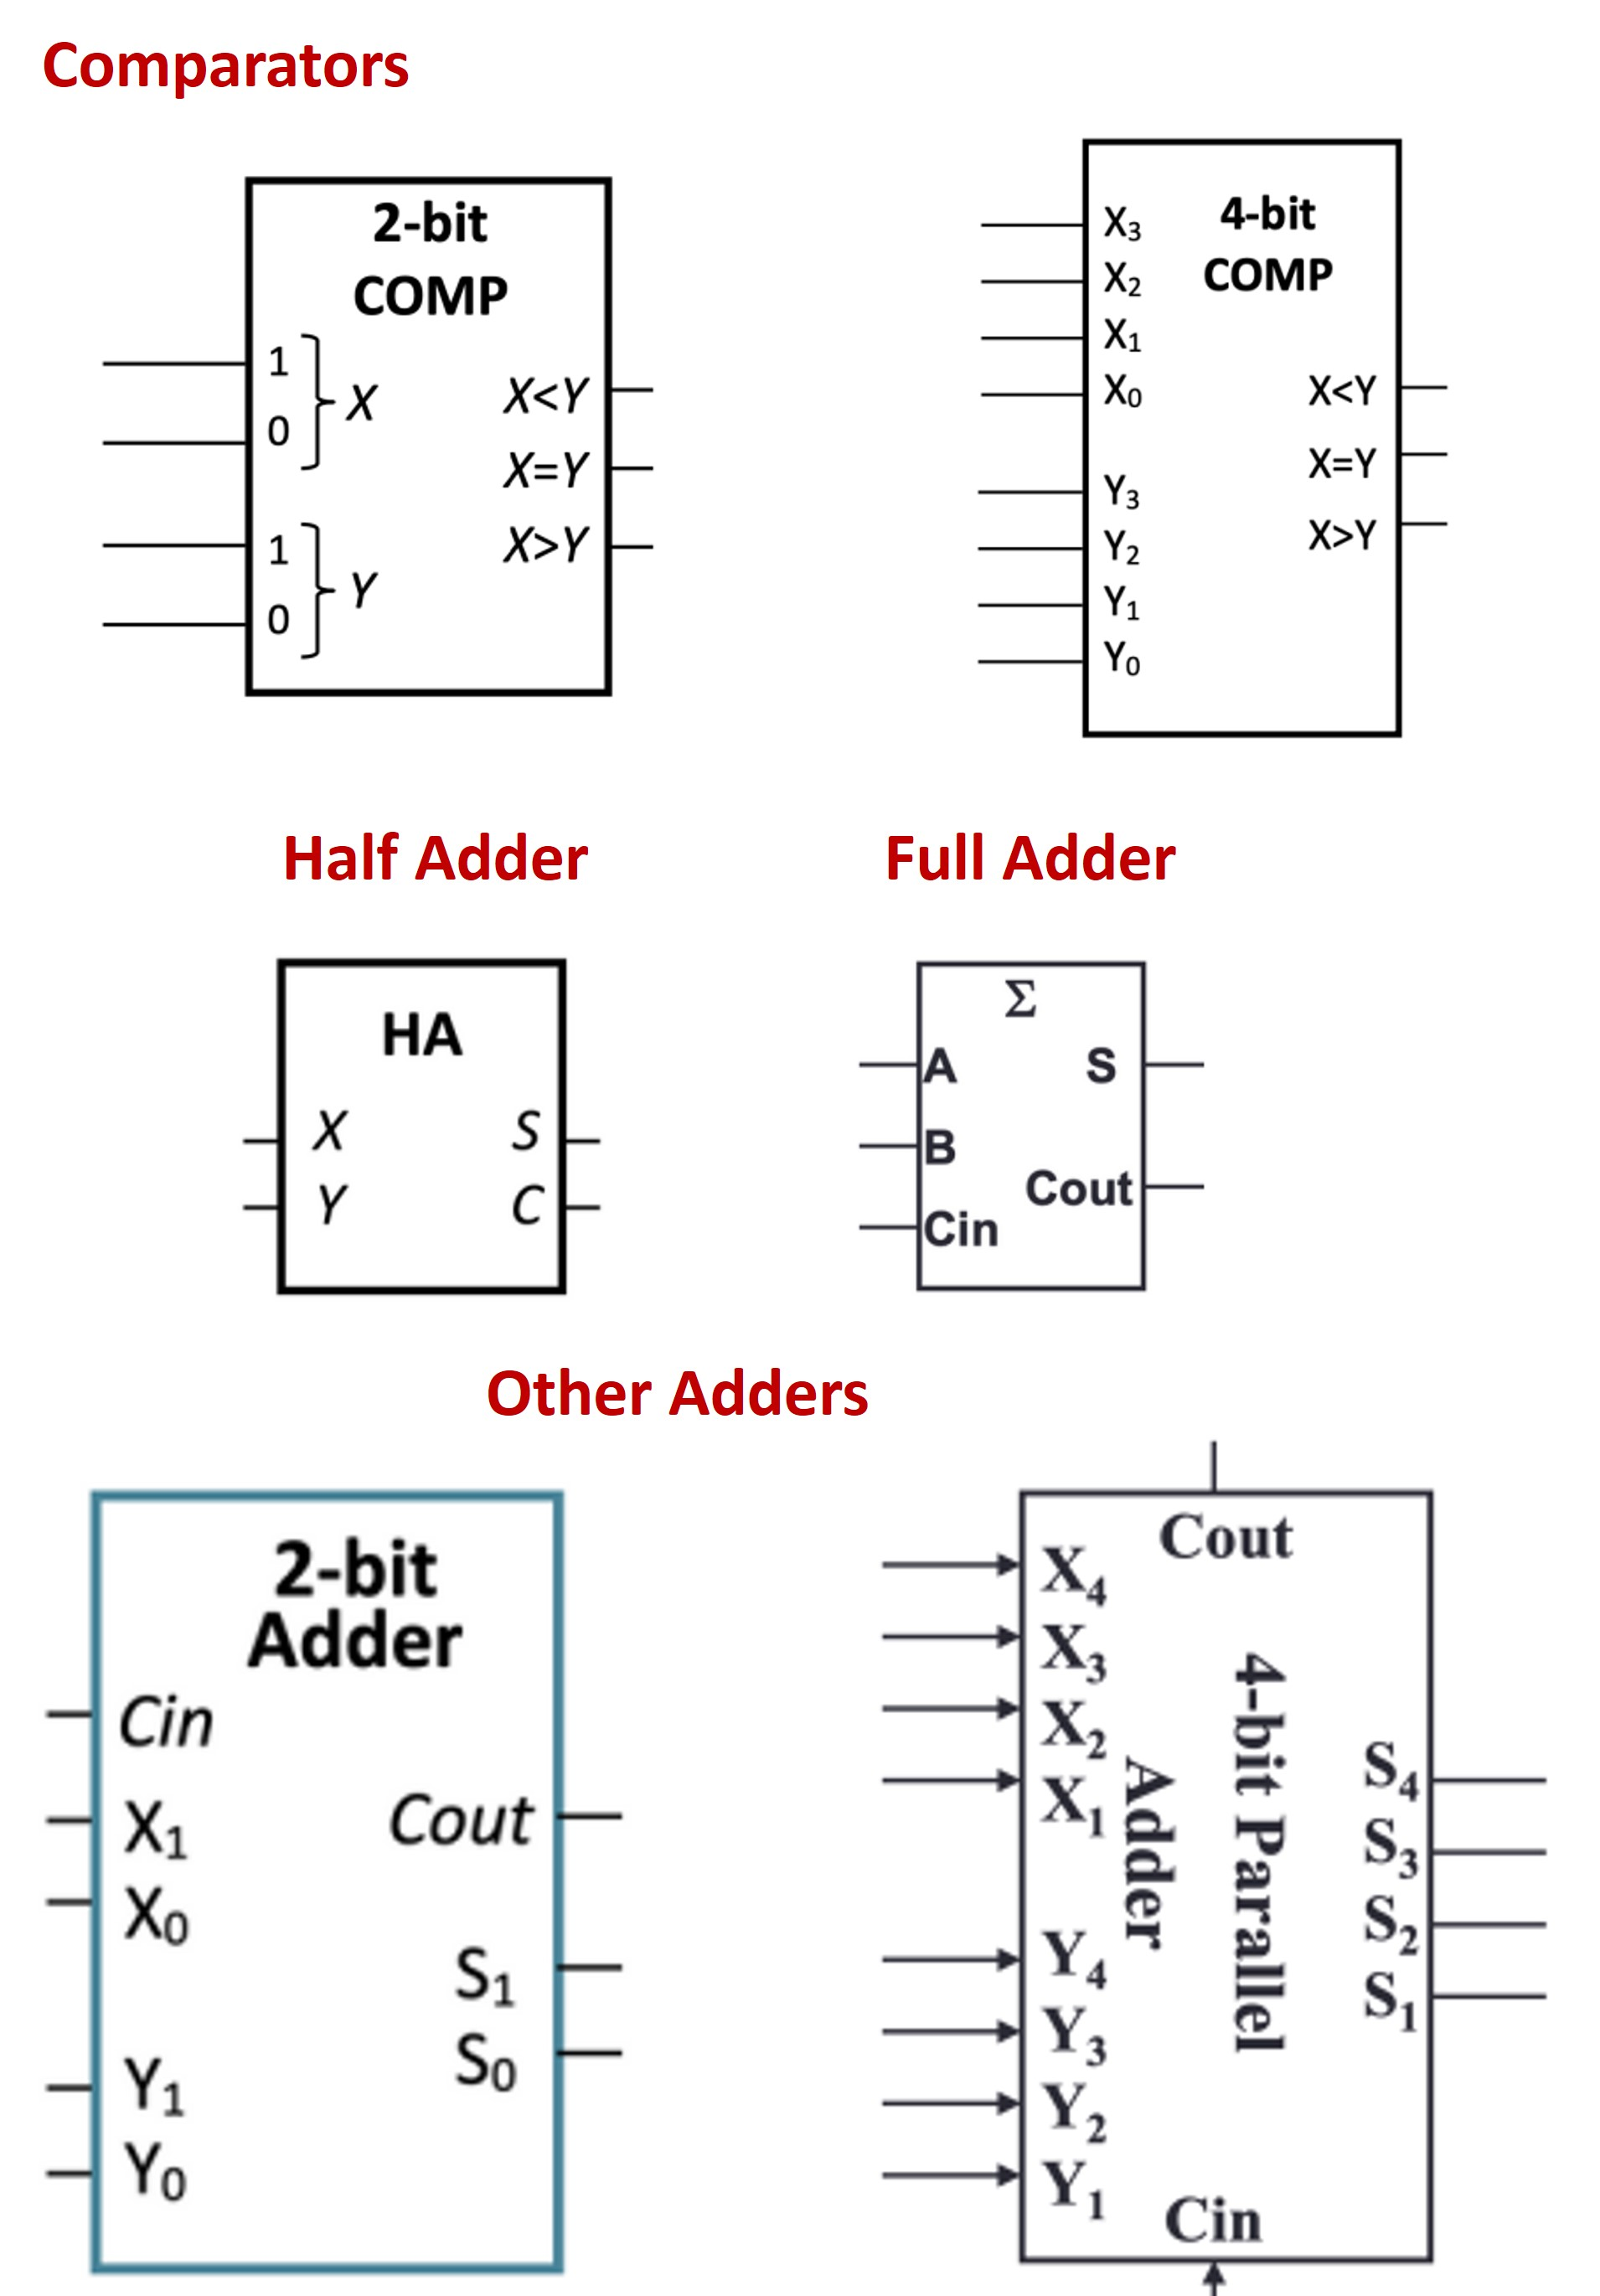
\includegraphics[width=0.8\linewidth]{block1}}

\subsubsection{MSI circuits Block Diagrams}
\centerline{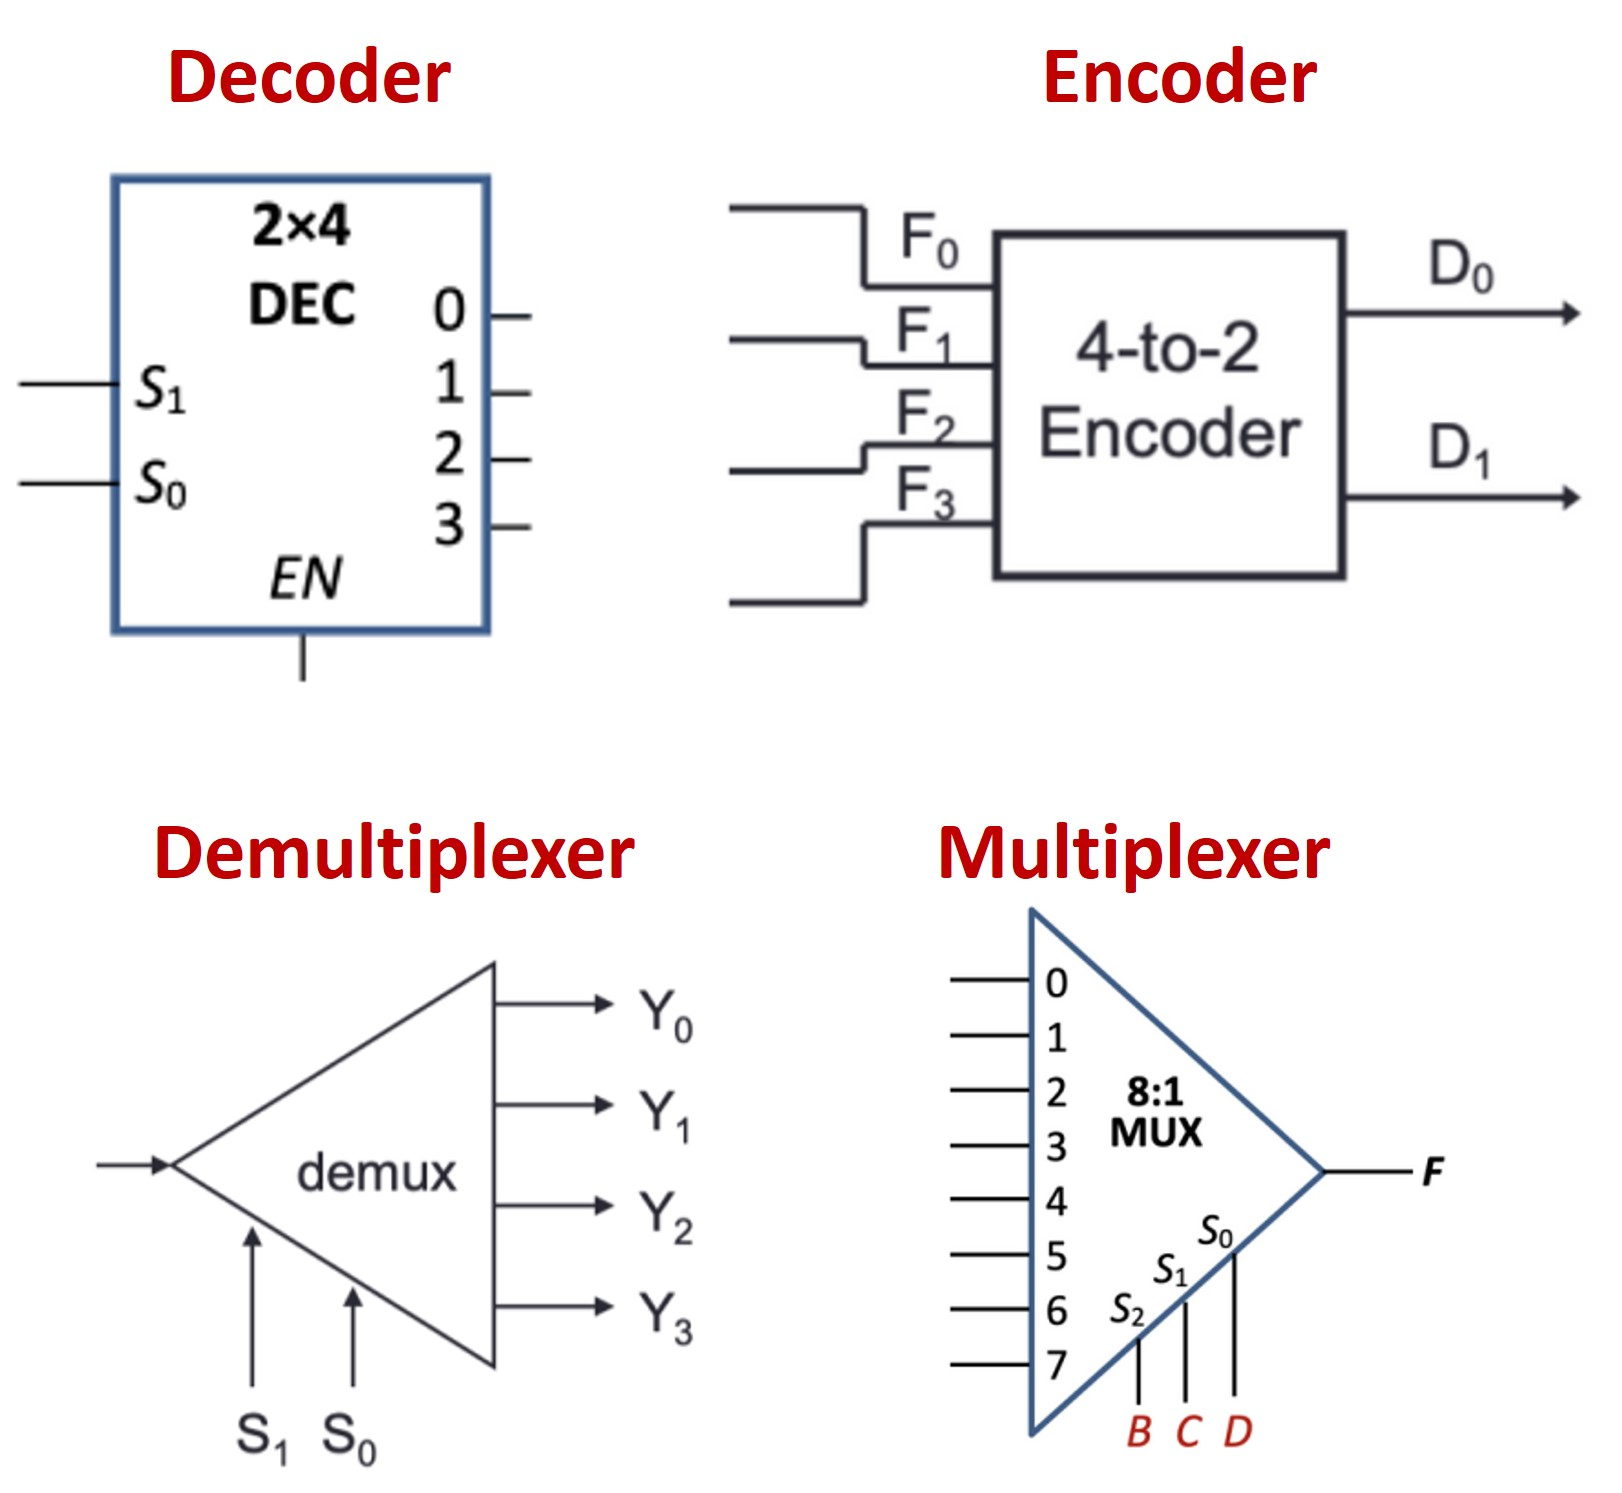
\includegraphics[width=0.8\linewidth]{msiblock}}


\columnbreak

\section{15. MSI Components}
\subsubsection{Integrated Circuit}
\begin{itemize}
\item \textbf{IC} aka chip or microchip is a set of electronic circuits on small flat piece of semiconductor.
\item \textbf{Scale of Integration}: No. of components on standard size IC. (SSI: Small-scale Integration, MSI: Medium, LSI: Large, VLSI: Very large, ULSI: Ultra-large).
\end{itemize}

\subsubsection{Decoders}
\begin{itemize}
\item convert binary information from $n$ input lines, to up to $2^n$ output lines
\item selects only one output line, aka $n$-to-$m$-line decoder, $n:m$ or $n x m$ decoder where $m \leq 2^n$.
\centerline{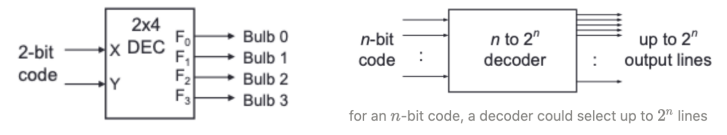
\includegraphics[width=1\linewidth]{decoder}}
\end{itemize}

\subsubsection{Encoders}
\begin{itemize}
\item given a set of input lines, of which exactly one is high and the rest are low, provide code that corresponds to the high input line.
\item opposite of decoder. $\leq 2^n$ input lines and n output lines
\item implemented with OR gates
\centerline{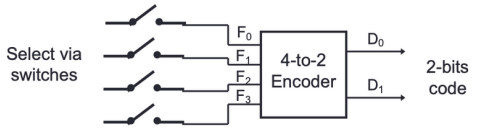
\includegraphics[width=0.8\linewidth]{encoder}}
\end{itemize}

\subsubsection{Priority Encoders}
\begin{itemize}
\item If multiple inputs are equal to 1, the highest \textbf{priority} takes precedence
\item all inputs 0: invalid input
\centerline{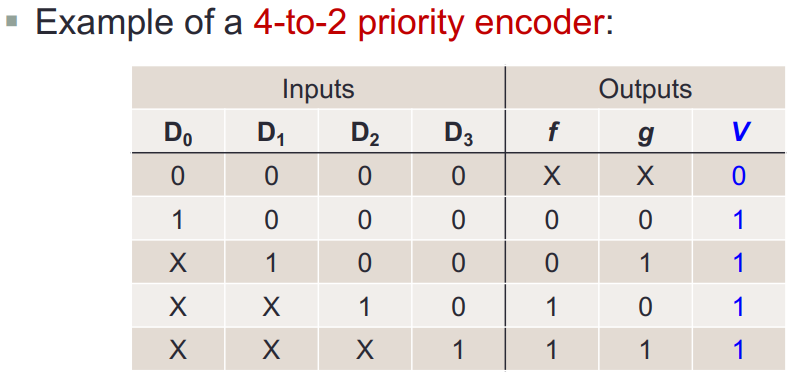
\includegraphics[width=0.7\linewidth]{pencoder}}
\end{itemize}

\subsubsection{Enable}
\begin{itemize}
\item \textbf{one-enable}: device is only activated when $E = 1$
\item \textbf{zero-enable:} device is only activated when $E = 0$, denoted or $E'$ or $\bar{E}$
\end{itemize}
\centerline{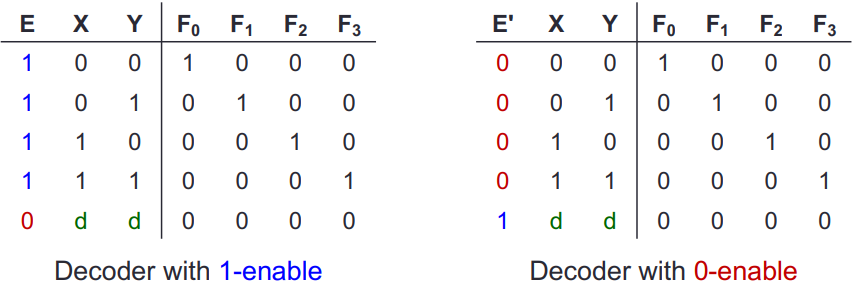
\includegraphics[width=0.7\linewidth]{enable}}

\subsubsection{Zero-Enable/Negated Outputs}
\begin{itemize}
\item \textbf{active-high outputs}: normal outputs (selected line is 1)
\item \textbf{active-low outputs}: negated outputs (selected line is 0)
\end{itemize}

\subsubsection{Implementing Functions with Decoders}
\begin{itemize}
\item any combinational circuit with inputs and outputs can be implemented with an $n:2^n$ decoder with $m$ OR gates.
\item \textbf{input}: bool function, in sum-of-minterms form
\item \textbf{output}: decoder for minterms, OR gate to form sum.
\end{itemize}
\centerline{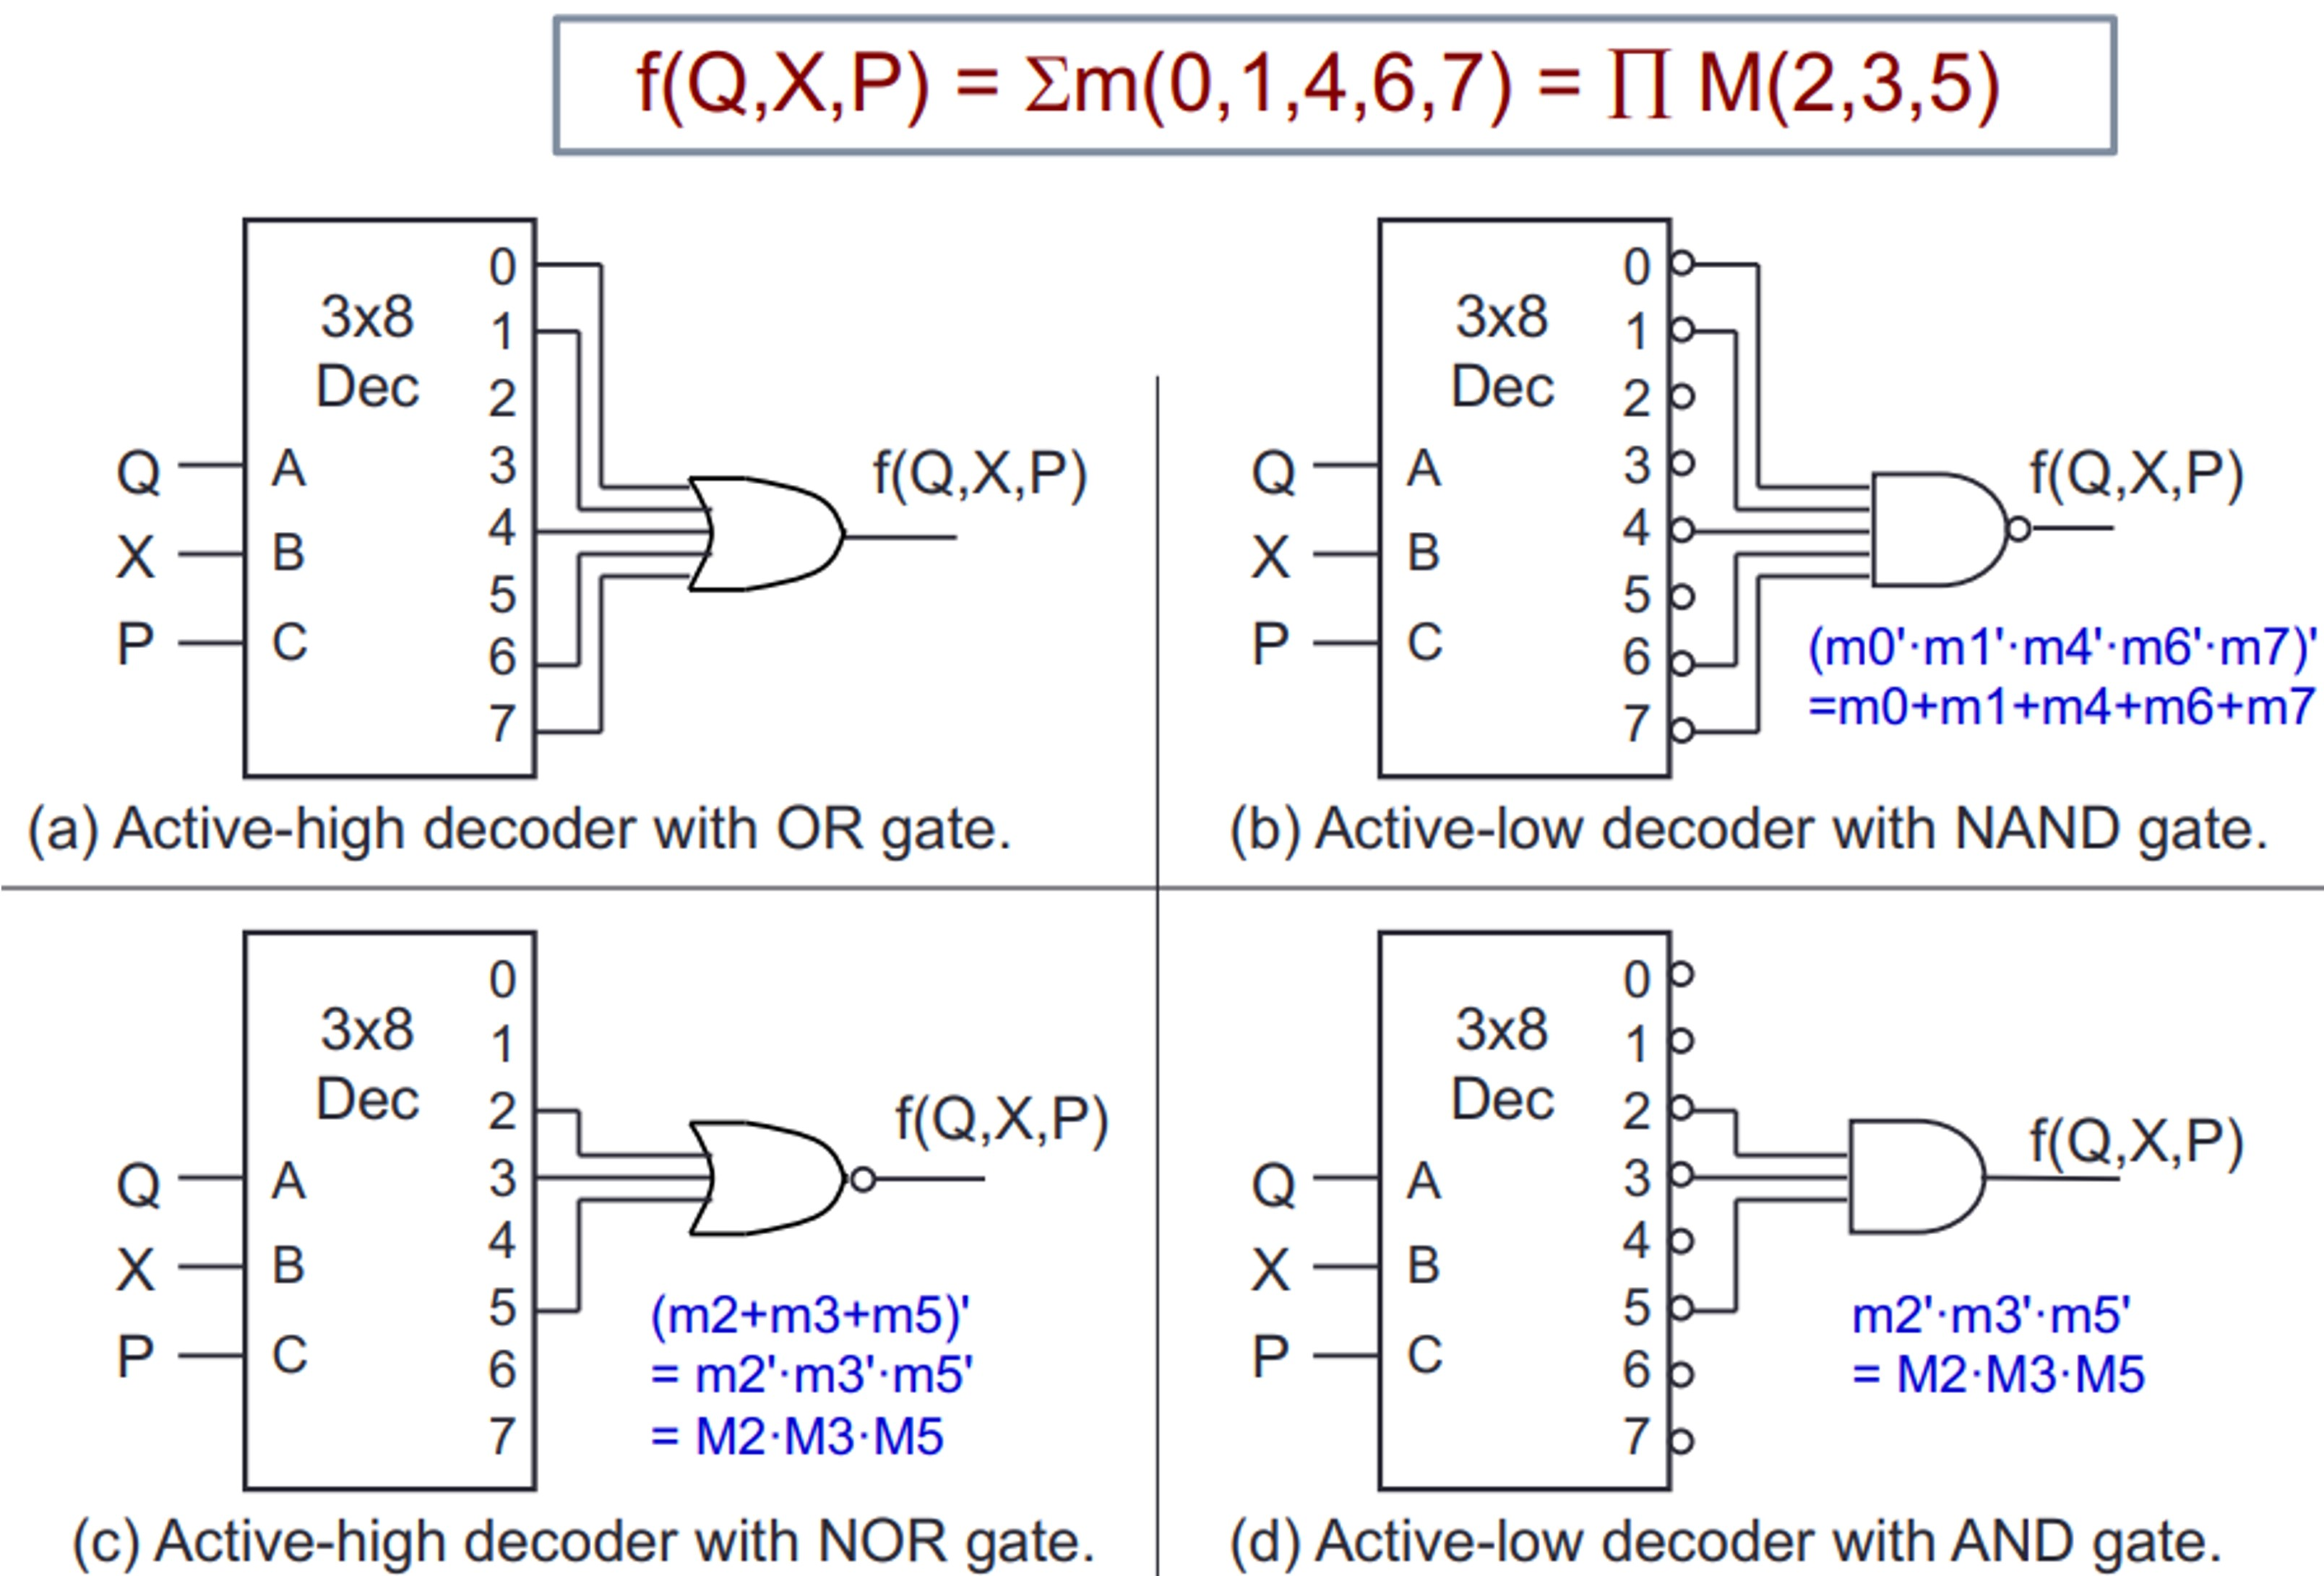
\includegraphics[width=1\linewidth]{decoderfunction}}

\subsubsection{Multiplexers \& Demultiplexers}
\centerline{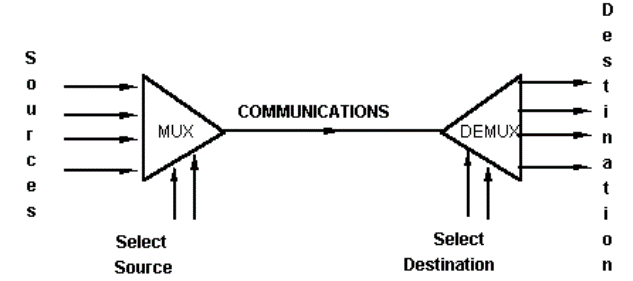
\includegraphics[width=0.5\linewidth]{mudemu}}
\begin{itemize}
\item Helps share \textbf{single comm line} among devices.
\item One source, one dest at a time. (Circuit switching)
\end{itemize}

\subsubsection{Demultiplexer}
\begin{itemize}
\item directs data from the input line to \textbf{one} selected output line
\item input: an input line and set of selection lines
\item "output": directs data to one selected line
\item \textbf{Identical} to a \textbf{decoder with enable}
\end{itemize}
\centerline{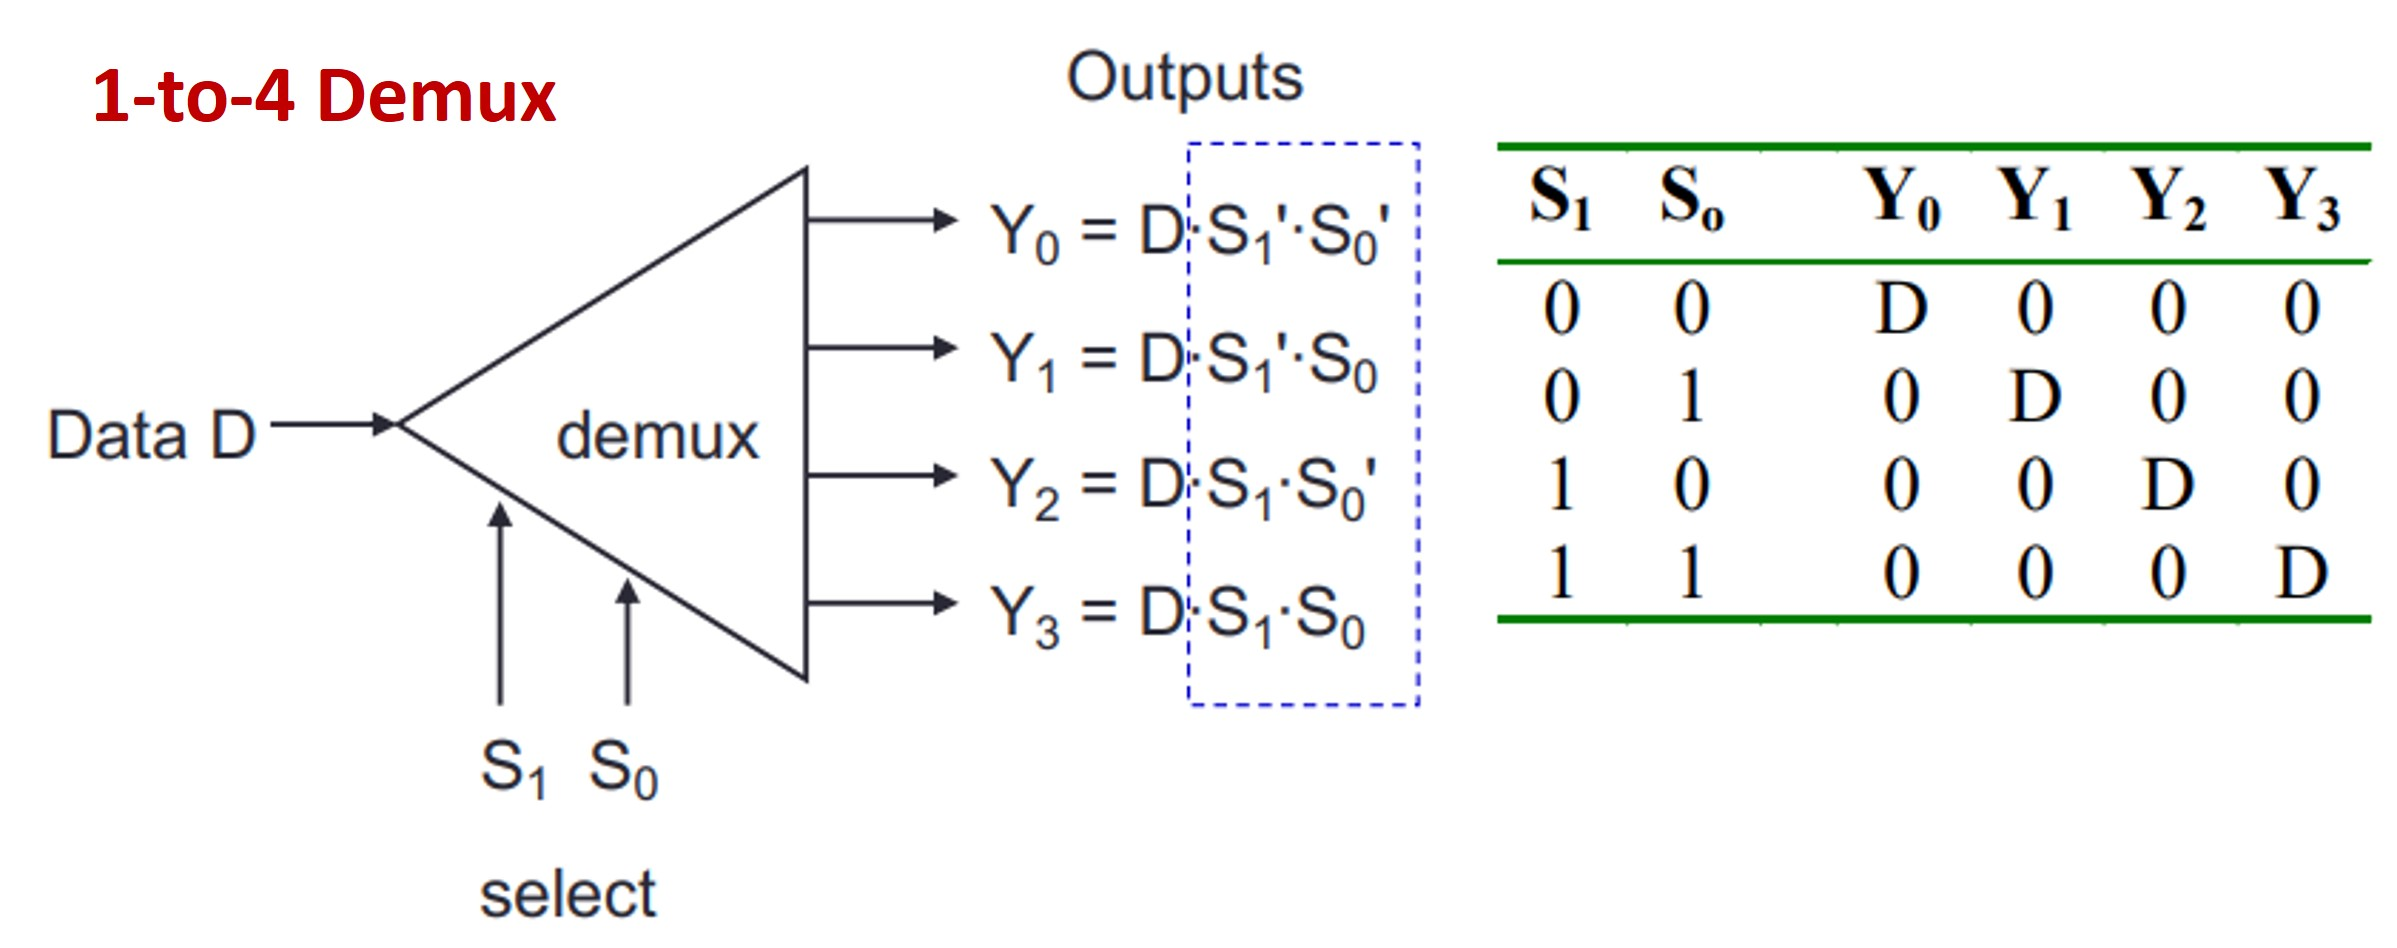
\includegraphics[width=0.8\linewidth]{demux}}

\subsubsection{Multiplexer}
\begin{itemize}
\item steers one of $2^n$ input lines to single output line, using selection lines.
\item \textbf{input}: multiple input lines, multiple selection lines
\item \textbf{output}: one output line $=$ sum of the (product of \underline{data lines} and \underline{selection lines})
\item  Larger multiplexers can be constructed from smaller ones.
\end{itemize}
\centerline{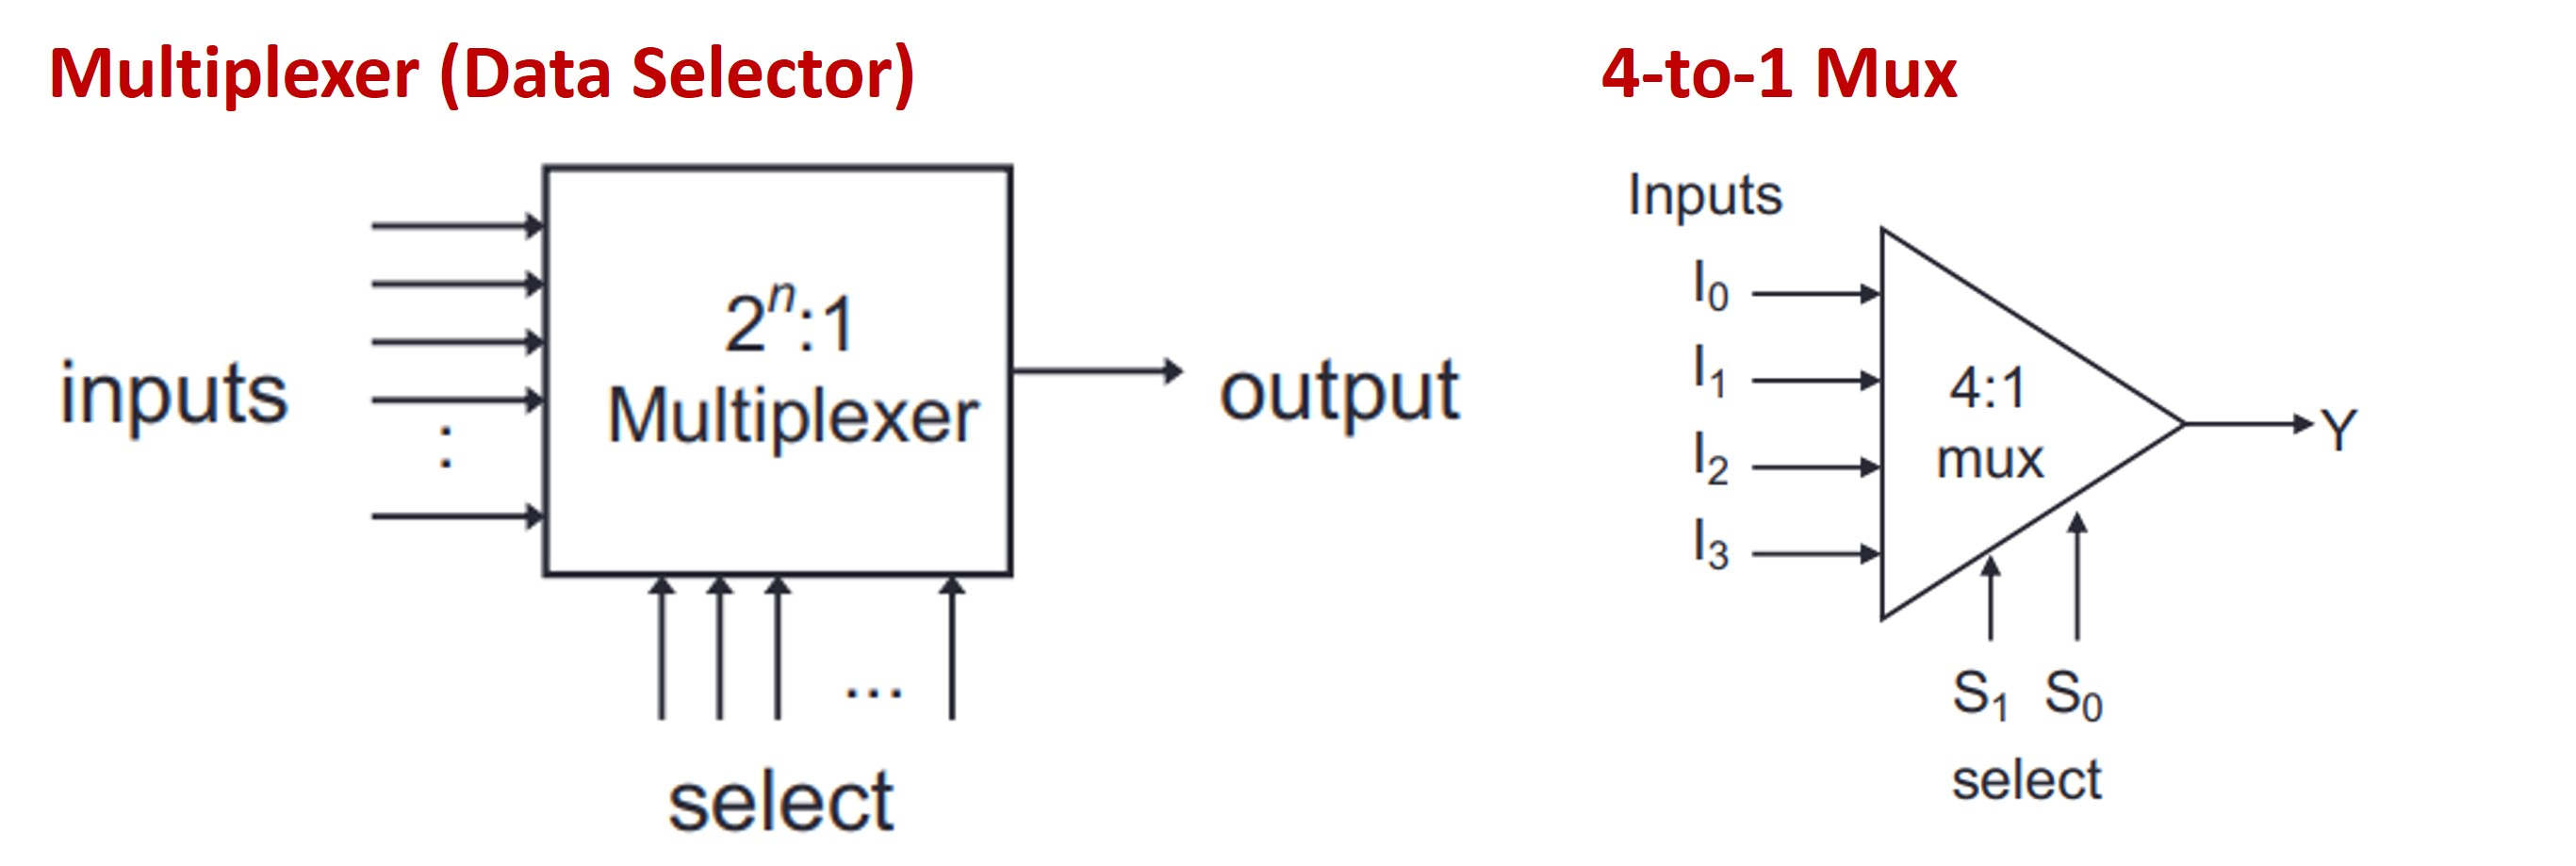
\includegraphics[width=0.8\linewidth]{mux}}

\subsubsection{Implementing Functions with Multiplexers}
\begin{itemize}
\item A $2^n$-to-$1$ multiplexer can implement bool function of $n$ input variables:
\item Express in sum-of-minterms form.
\item Connect $n$ variables to $n$ selection lines, put ‘1’ on data line if minterm of function, ‘0’ otherwise
\end{itemize}
\centerline{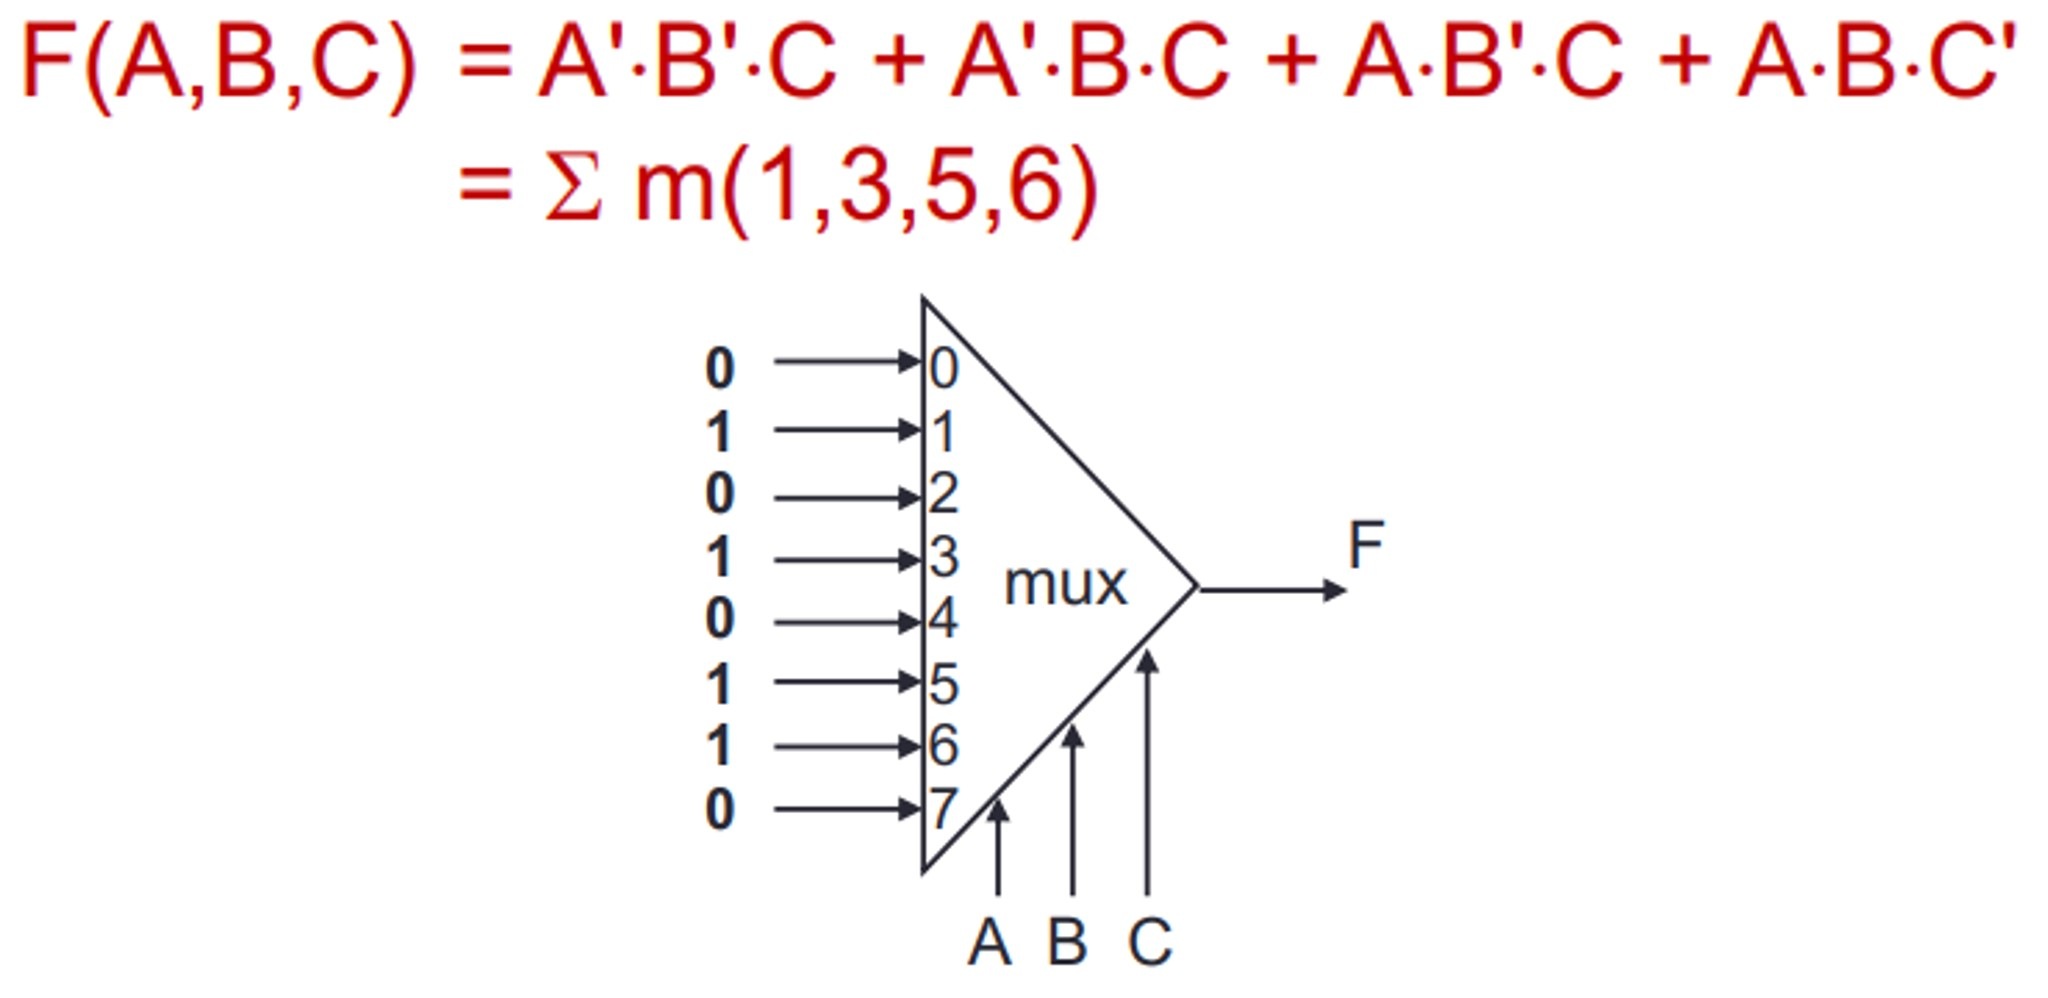
\includegraphics[width=0.8\linewidth]{muxfun}}

\subsubsection{Using smaller multiplexers for Functions}
\begin{itemize}
\item We can use single smaller $2^{(n-1)}-to-1$ multiplexer to implement bool function of $n$ (input) variables.
\item \textbf{Procedure:} Express function in sum-of-minterms form, reserve one variable (here take least significant one) for input lines of multiplexer, and 
use rest for selection lines. (C for input, A \& B for selection)
\item Draw truth table for function, group inputs by selection line values, determine multiplexer inputs by comparing input line (C) and function (F).
\end{itemize}
\centerline{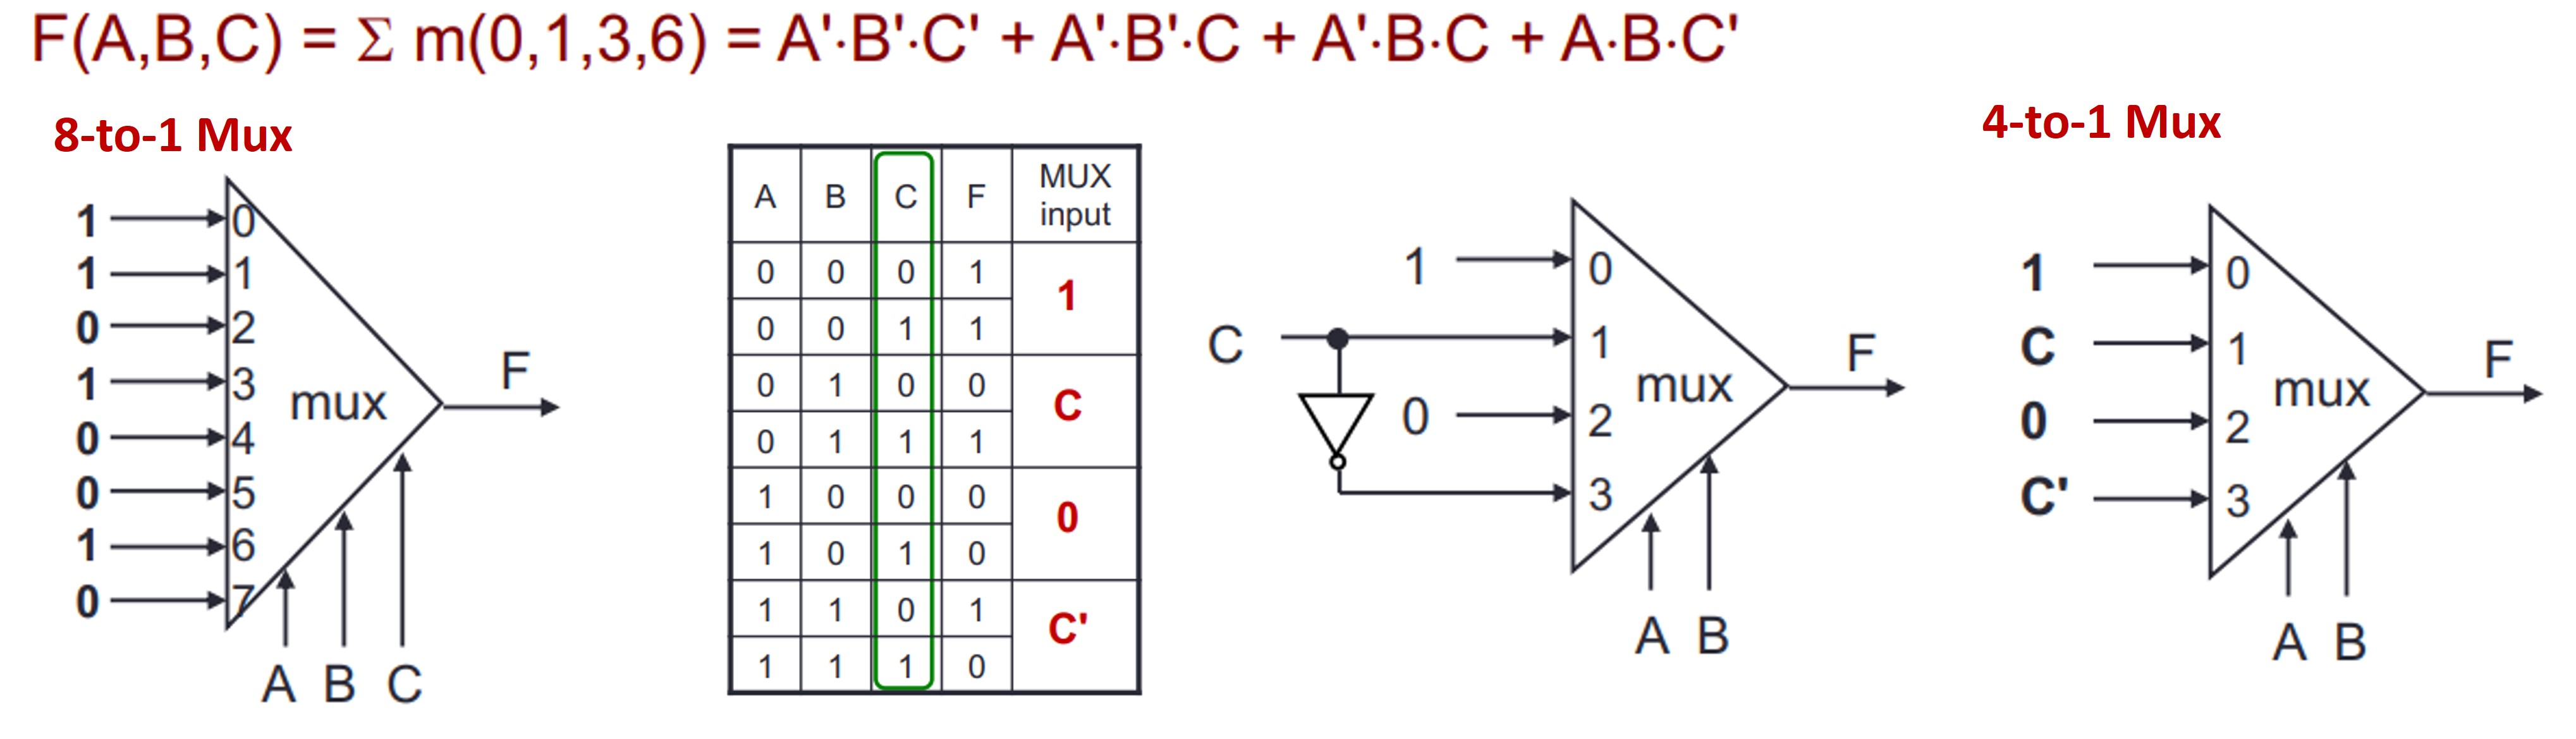
\includegraphics[width=1\linewidth]{smallermux}}

\vfill \null
\columnbreak

\section{16. Sequential Logic}
\begin{itemize}
\item \textbf{Sequential Circuit}: output depends on both \underline{present inputs} and  \underline{state}
\item 2 Types of sequential circuits: \\ 
\textbf{synchronous}: outputs change only at a specific time \\
\textbf{asynchronous}: outputs change at any time
\item Classes of sequential circuits: \\
\textbf{bistable}: 2 stable states (e.g. latches / flip-flops)
\textbf{monostable}: 1 stable state; astable, no stable state
\end{itemize}

\subsubsection{Latches}
\begin{itemize}
\item pulse-triggered (vs flipflops: edge-triggered)
\end{itemize}

\subsubsection{Flip-Flops}
\begin{itemize}
\item \textbf{synchronous bistable devices}: data on inputs is transferred to the flipflop's output only on the triggered edge of the clock pulse.
\item output changes state at a \underline{specific point on the clock}: \\
change state at either rising or falling edge of the clock signal
\end{itemize}

\subsection{Memory Elements}
\begin{itemize}
\item \textbf{Memory Elements}: Device which can remember value indefinitely, or change value on command from its inputs.
\end{itemize}
\centerline{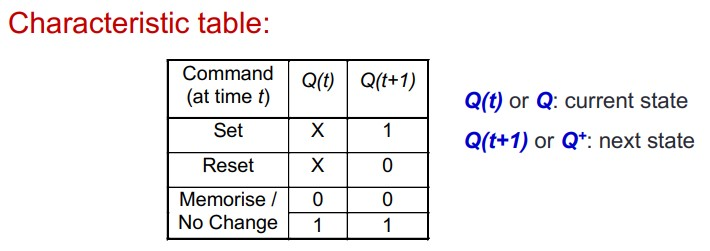
\includegraphics[width=0.8\linewidth]{memoryelement}}
\subsection{Memory Elements with Clock}
\begin{itemize}
\item\textbf{pulse-triggered}: ON = 1, OFF = 0
\item \textbf{edge-triggered}:
\begin{enumerate}
\item \textbf{positive edge-trig}: ON: from 0 to 1, OFF: other t.
\item \textbf{negative edge-trig}: ON: from 1 to 0, OFF: other t.
\end{enumerate}
\end{itemize}
\centerline{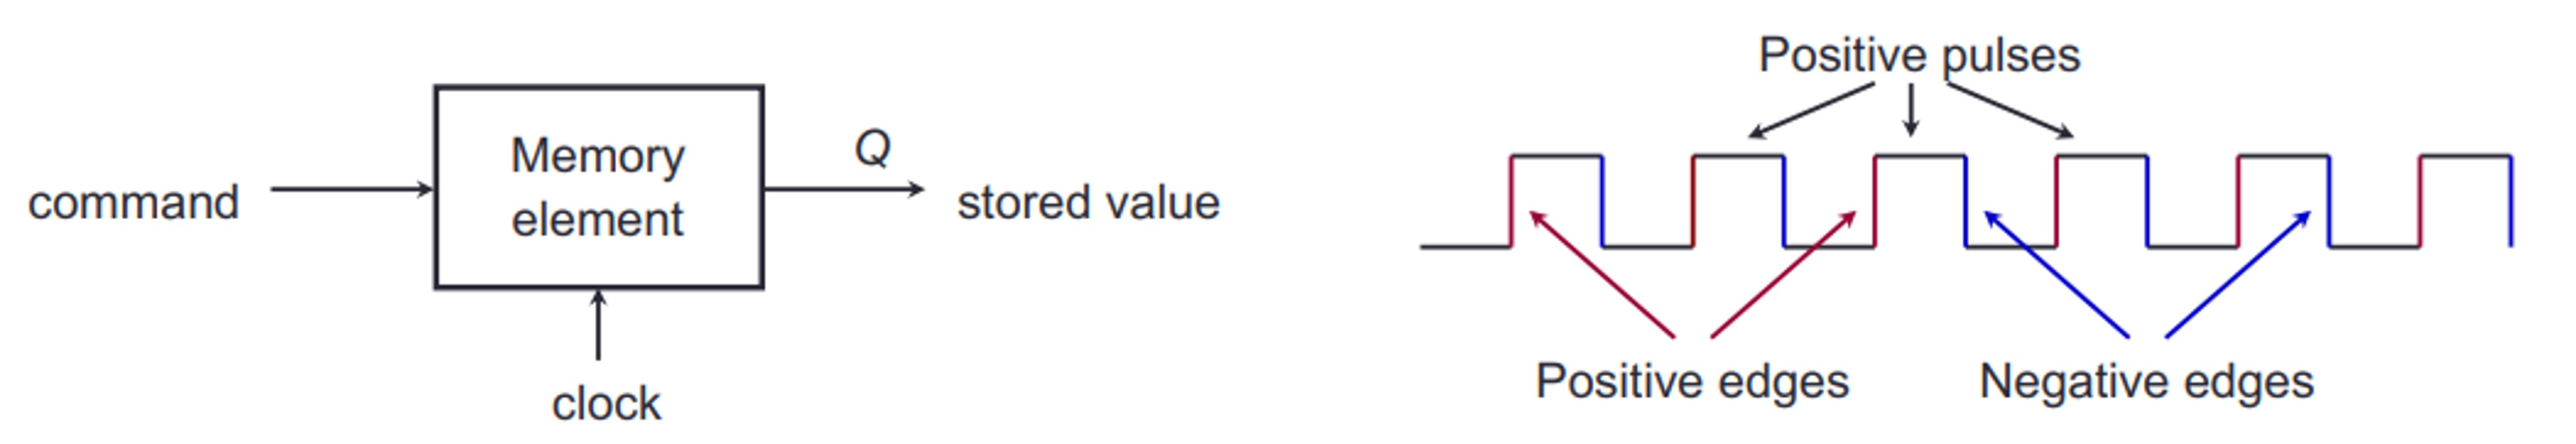
\includegraphics[width=1\linewidth]{memoryelementclock}}

\subsection{Latches}
A Latch is a \textbf{sequential circuit} that watches all inputs continuously and changes output at any time \textbf{independently of a clocking signal}.

\subsubsection{S-R Latch}
\begin{itemize}
\item Two \textbf{Inputs}: $S$ (Set) and $R$ (Reset).
\item 2 complementary \textbf{outputs}: $Q$ and $Q'$
\item When $Q =$ high, latch is in SET state.
\item When $Q =$ low, latch is in RESET state.
\end{itemize}
\centerline{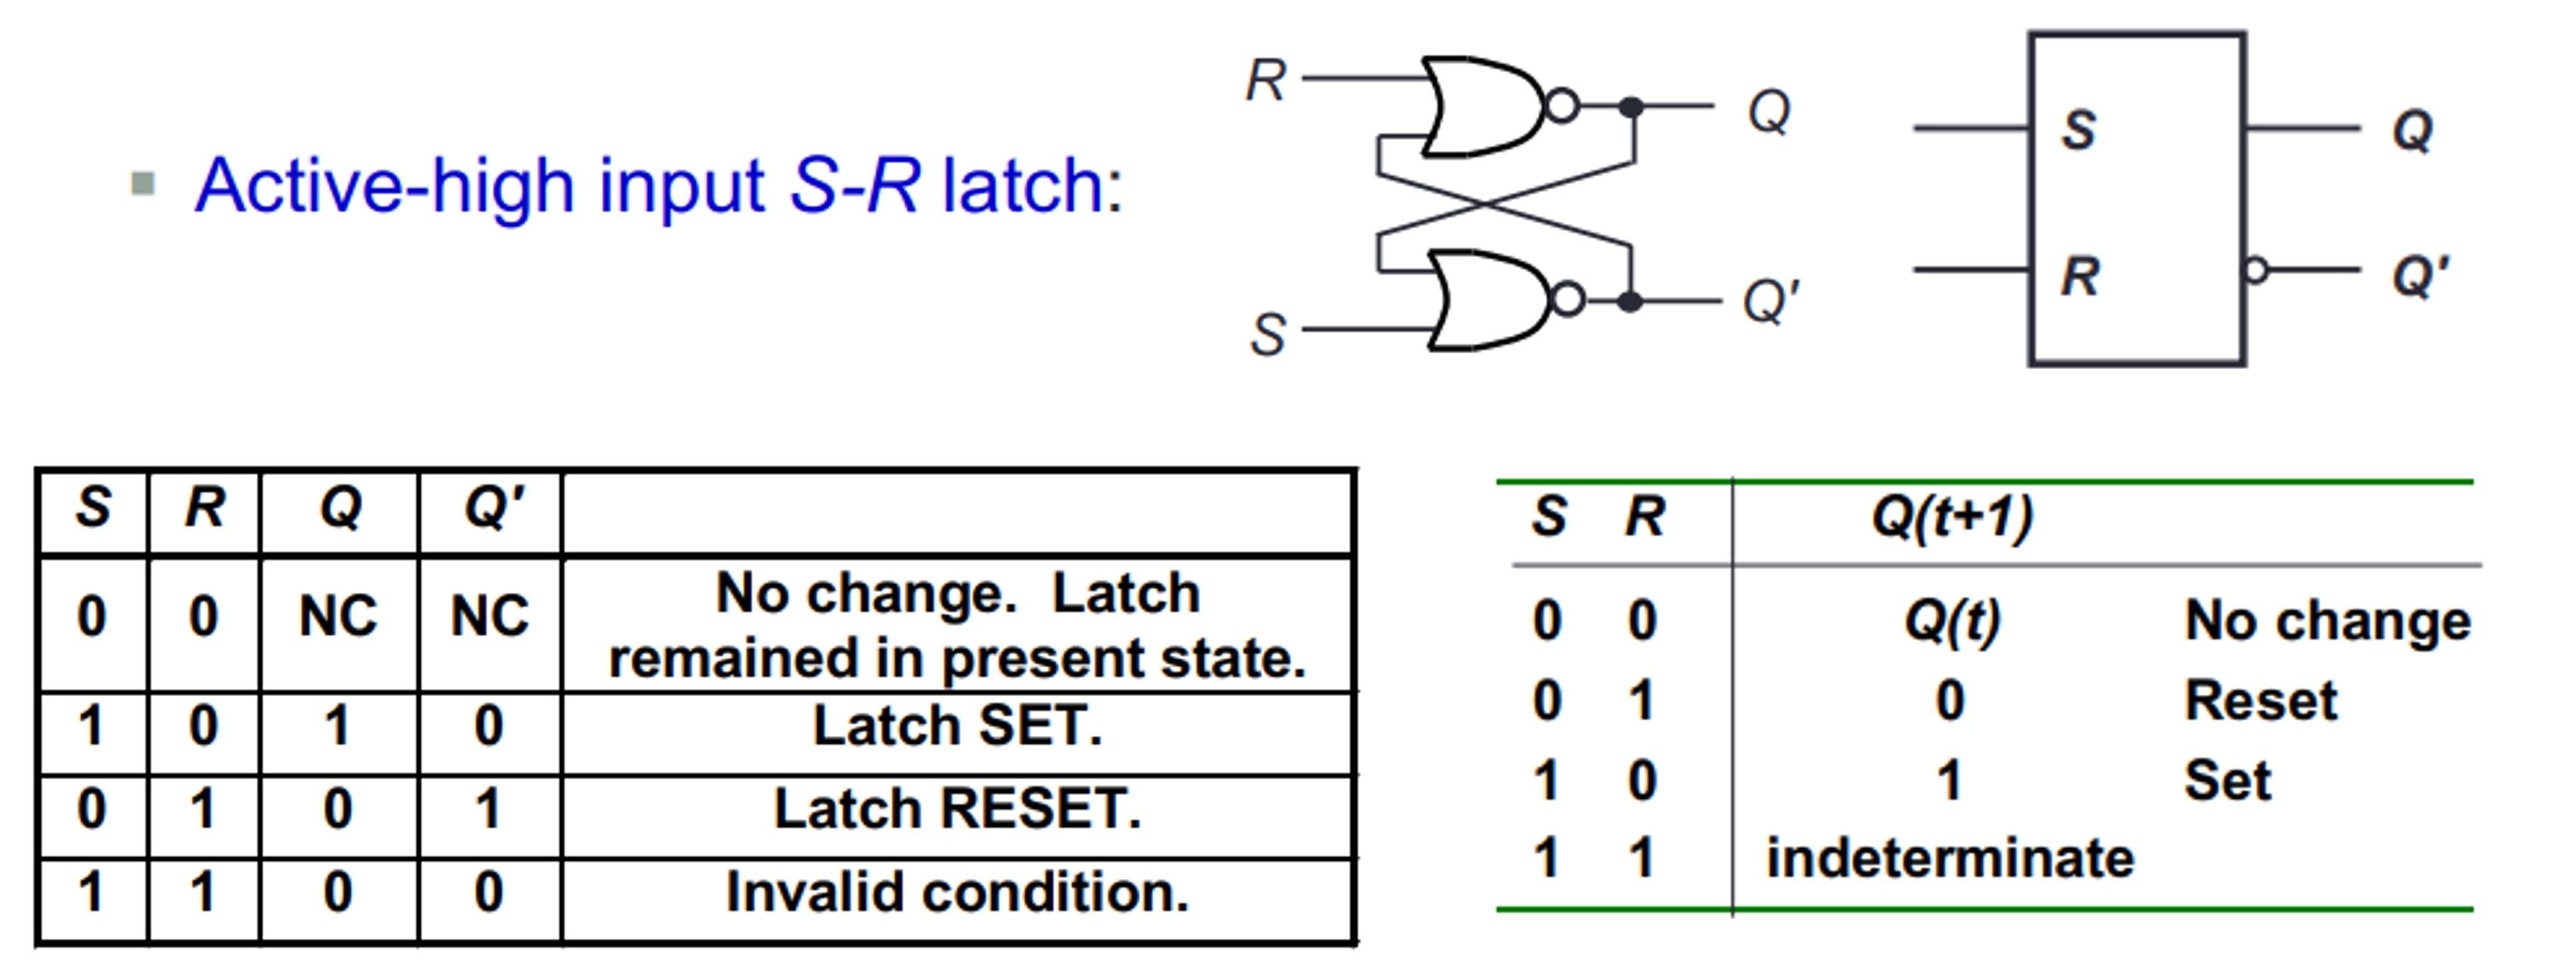
\includegraphics[width=1\linewidth]{SRlatch}}

\subsubsection{Gated S-R Latch}
\begin{itemize}
\item \textbf{S-R Latch + enable input (EN) + 2 NAND gates}
\item outputs change only when EN is high
\end{itemize}
\centerline{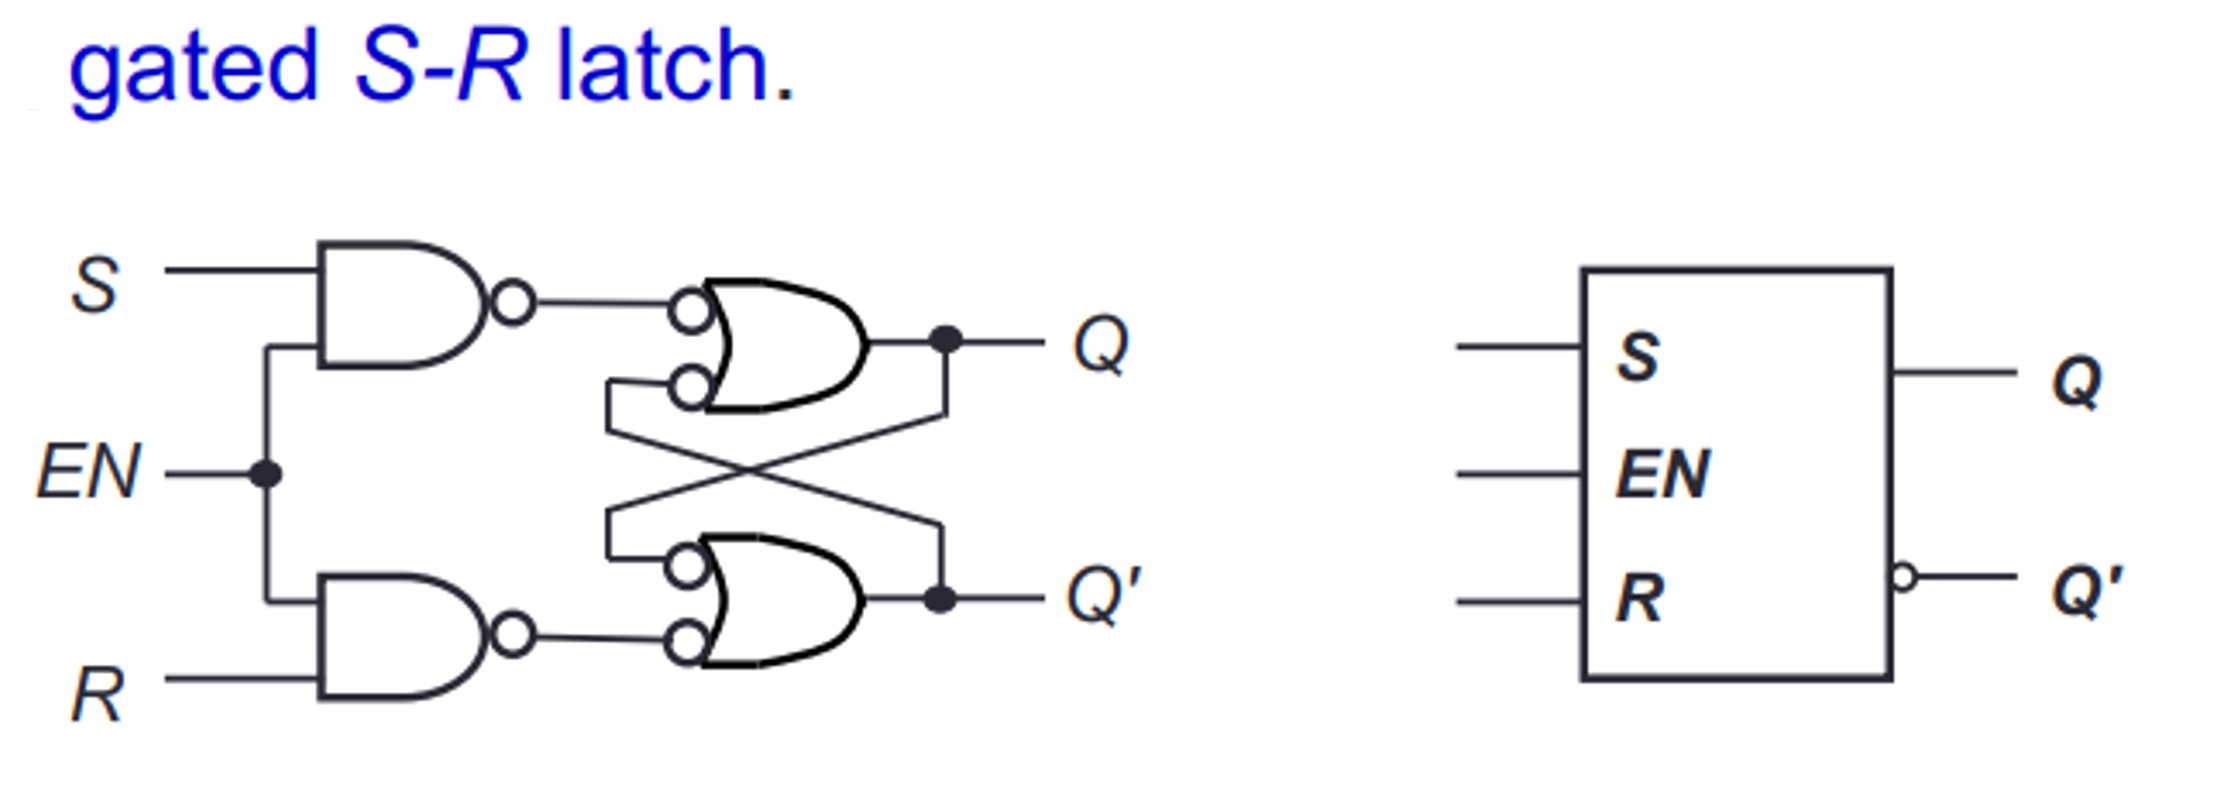
\includegraphics[width=0.8\linewidth]{gatedSRlatch}}

\subsubsection{Gated D Latch}
\begin{itemize}
\item \textbf{Gated D latch} make $R$ input equal to $S'$
\item eliminates undesirable condition of invalid state in the S-R latch.
\end{itemize}
\centerline{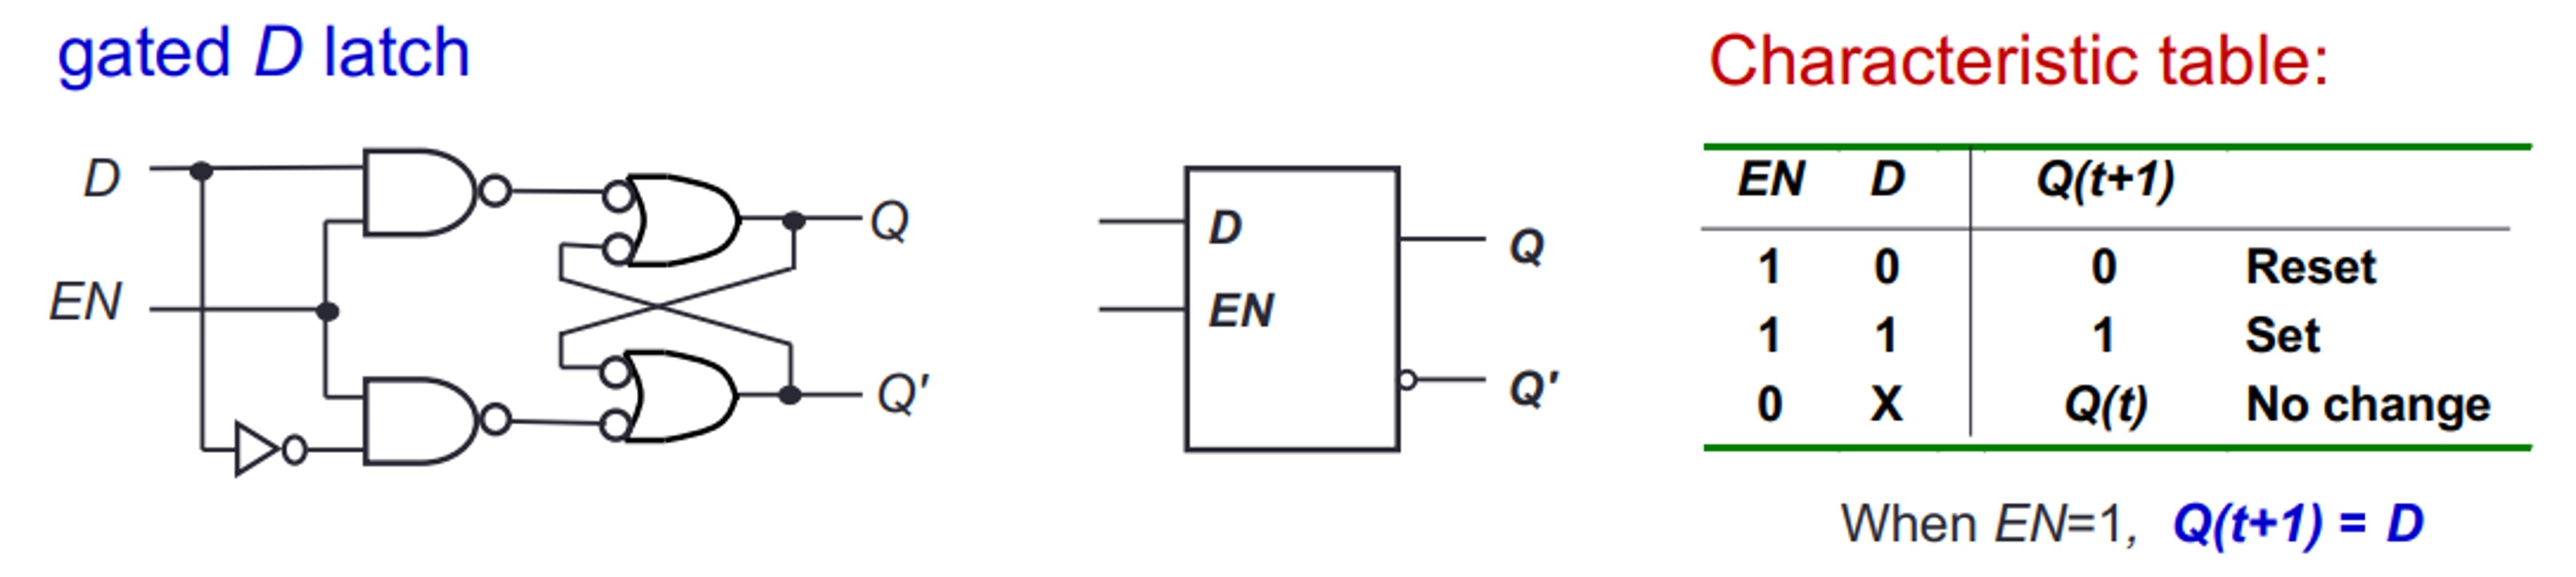
\includegraphics[width=1\linewidth]{gatedDlatch}}

\columnbreak

\subsection{Flip-flops}
Flip-flops changes its outputs only at times determined by a clocking signal. AKA basic digital memory circuit.

\subsubsection{S-R flip flop}
\begin{itemize}
\item $>$ symbol at clock input. Negative edge-trigger: $\circ>$. Outputs change at triggering edge of clock pulse. 
\end{itemize}
\centerline{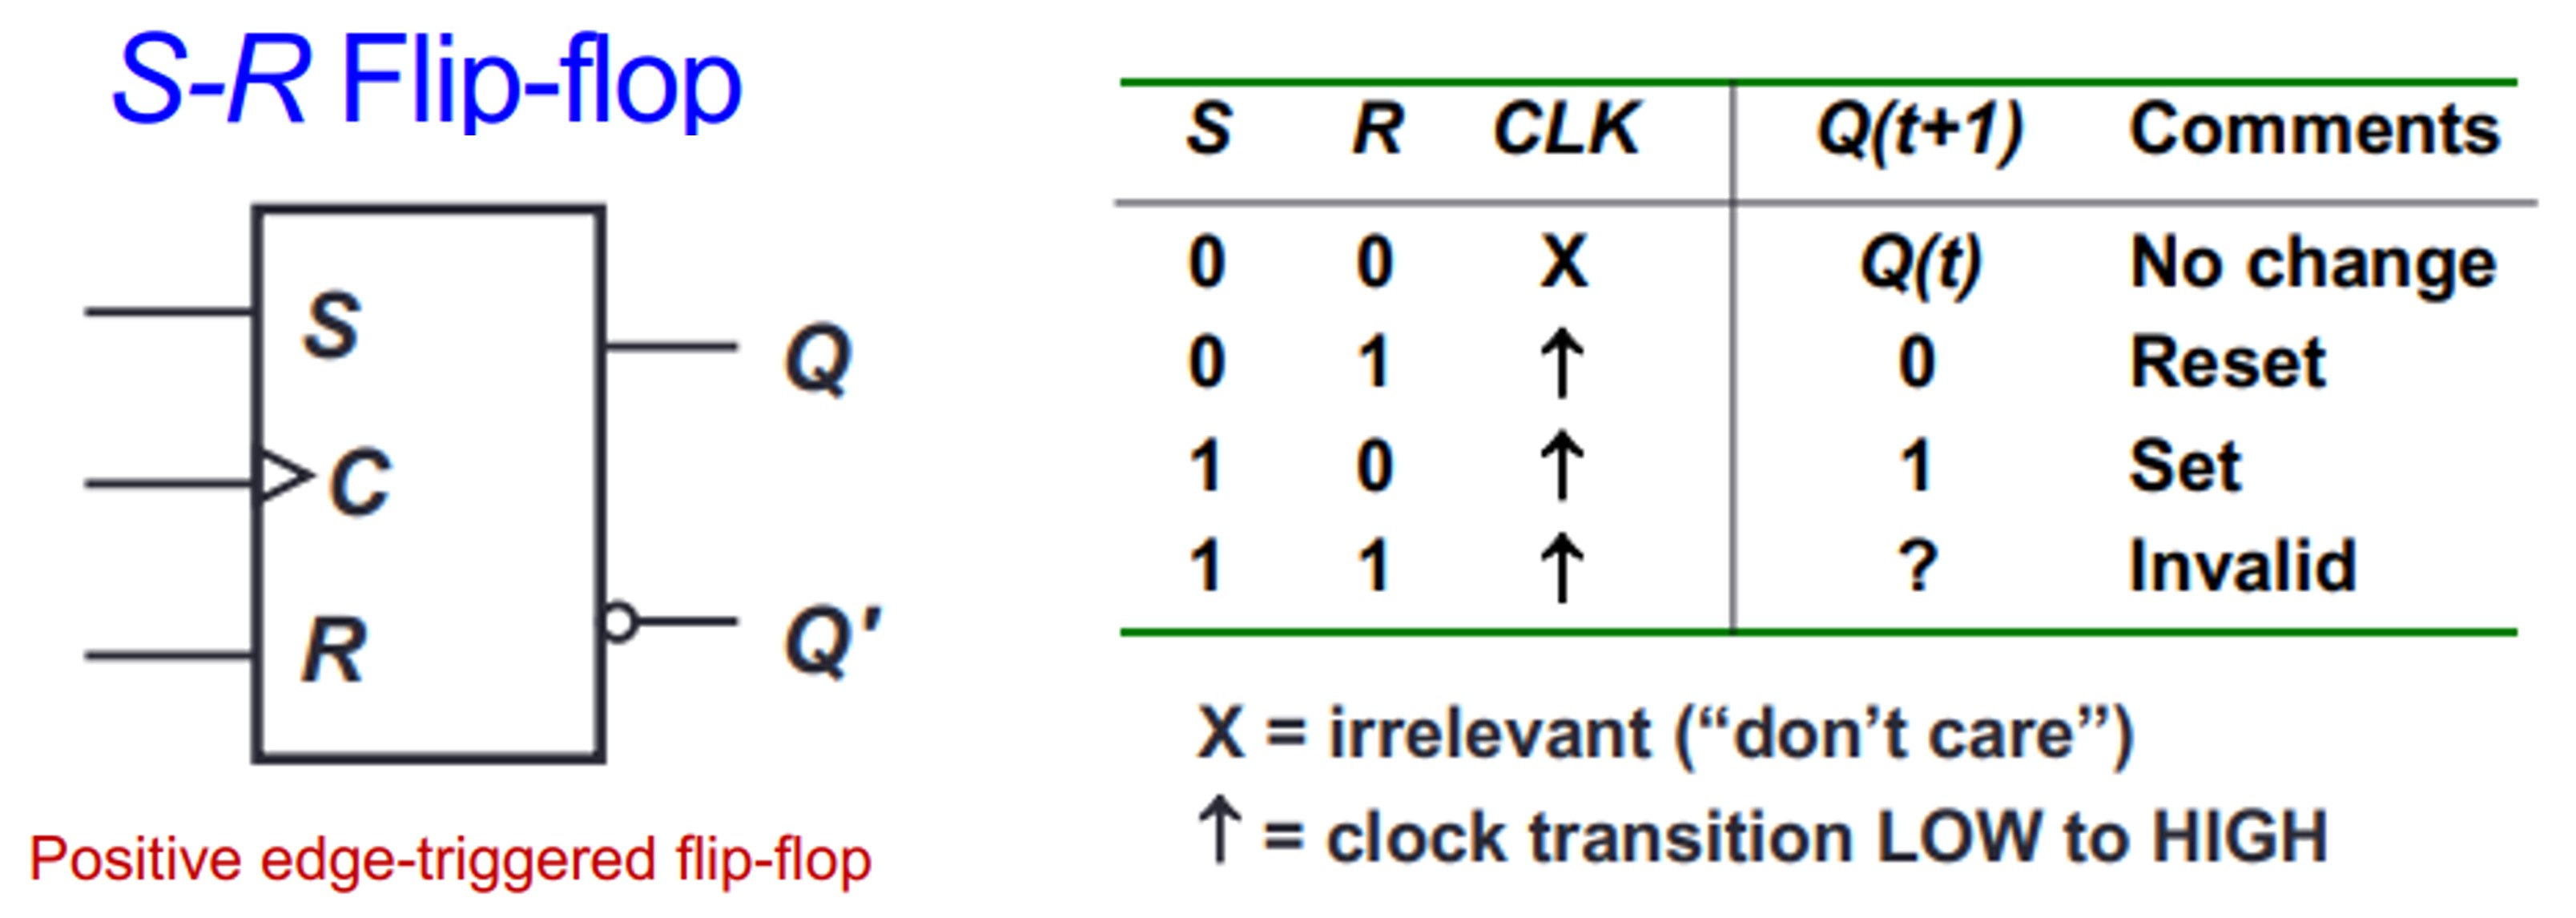
\includegraphics[width=1\linewidth]{SRflipflop}}

\subsubsection{D flip flop}
\centerline{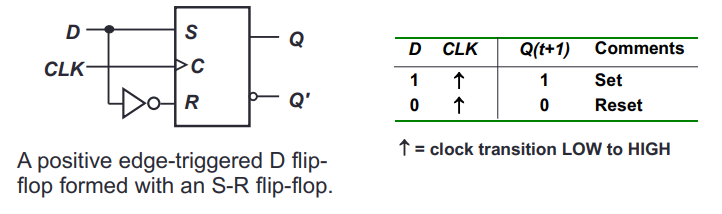
\includegraphics[width=1\linewidth]{dflipflop}}

\subsubsection{J-K flip flop}
\begin{itemize}
\item No valid state, Includes \textbf{toggle} state: $Q$ changes on each active clock edge.
\end{itemize}
\centerline{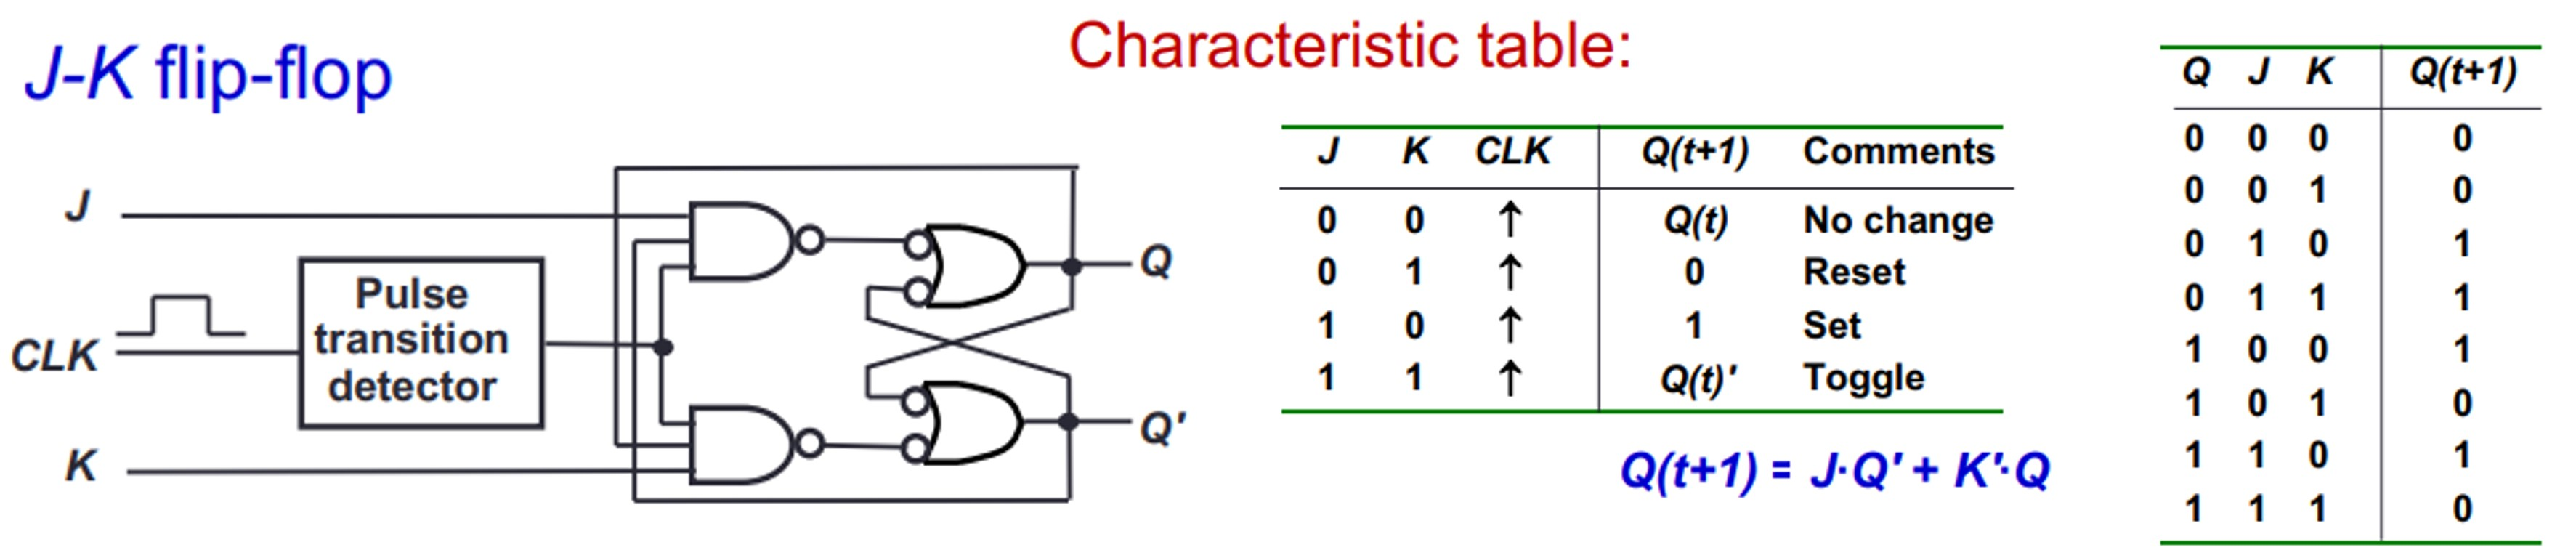
\includegraphics[width=1\linewidth]{jkflipflop}}

\subsubsection{T flip flop}
\begin{itemize}
\item \textbf{T flip-flop}: Single input version of the J-K flip-flop, formed 
by tying both inputs together.
\item $Q(t + 1) = T \oplus Q$
\end{itemize}

\centerline{\includegraphics[width=0.9\linewidth]{tflipflop}}

\section{Asynchronous Inputs}
\begin{itemize}
\item \textbf{asynchronous} inputs affect the state of the flip-flop independent of the clock.
\item e.g. J-K flip-flop with active-low PRESET and CLEAR asynchronous input
\end{itemize}
\centerline{\includegraphics[width=1\linewidth]{jkflipflopasync}} 
For \textbf{active-high}:
\begin{itemize}
\item PRE = 1 (HIGH): Q immediately set to HIGH
\item CLR = 1 (HIGH): Q immediately cleared to LOW
\item normal operation mode: both PRE and CLR are LOW
\end{itemize}

\section{Synchronous Sequential Circuits}
\begin{itemize}
\item Building blocks: \textbf{logic gates \& flip flops}. 
\item Flip-flops make up the memory, while gates form combinational sub-circuits.
\end{itemize}

 \null \null \null \null \null \null

\columnbreak

\subsection{Flip Flop Characteristic Tables}
\textbf{Characteristic tables} are used in analysis.
\centerline{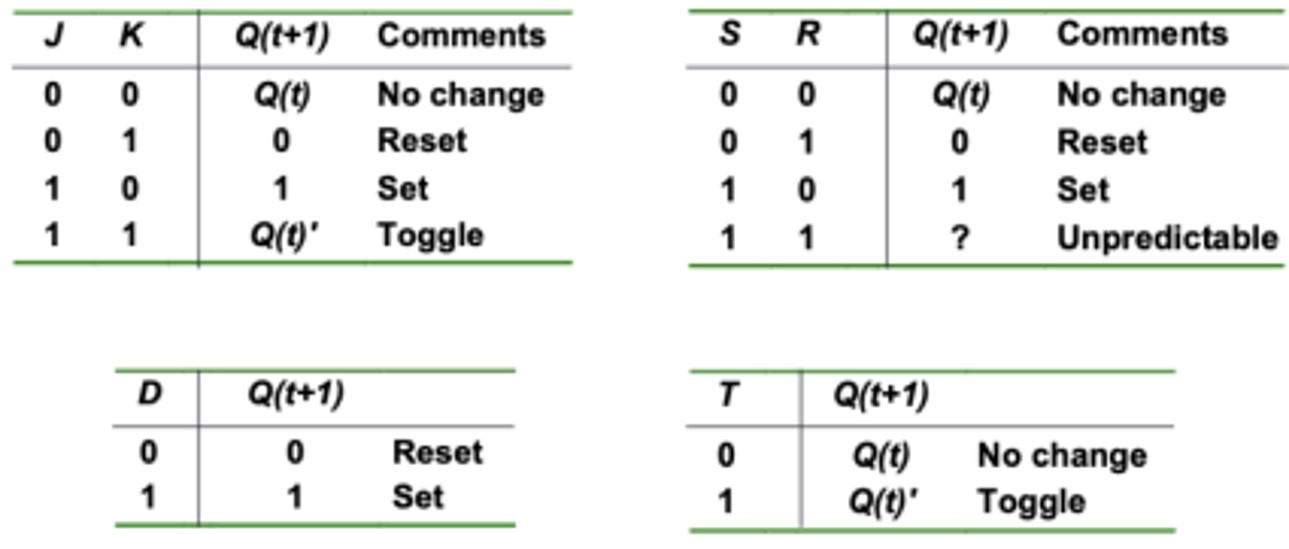
\includegraphics[width=1\linewidth]{flipflopctable}} 

\subsection{Flip Flop Excitation Tables}
\textbf{Excitation tables} are used in design.
\centerline{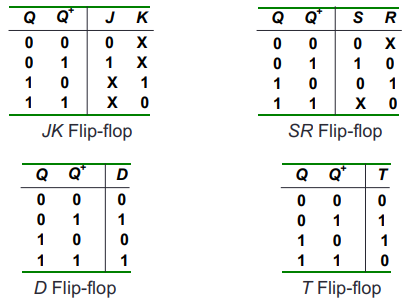
\includegraphics[width=1\linewidth]{excitationtables}} 

 \null \null \null \null \null \null
 \null \null \null \null \null \null

\columnbreak

\section{17. Sequential Circuits Design}

\textbf{Sequential Circuits Design}: \textit{(from state equations/table/diagram to logic circuit).}
\begin{itemize}
\item For unused states, use \textbf{don't care X} for input.
\item \textbf{Self-correcting}: any unused state can transition to a used state after a finite number of cycles
\end{itemize}
\begin{enumerate}
\item Convert state diagram to state table.
\item fill in flip-flop inputs based on excitation table
\item use K-maps to get simplified logic expressions for flip-flop inputs (e.g.
JA, KA, JB, KB)
\item draw circuit implementing
\end{enumerate}

\subsubsection{Example}
\textbf{State diagram, design seq circuit with JK flip-flops}
\centerline{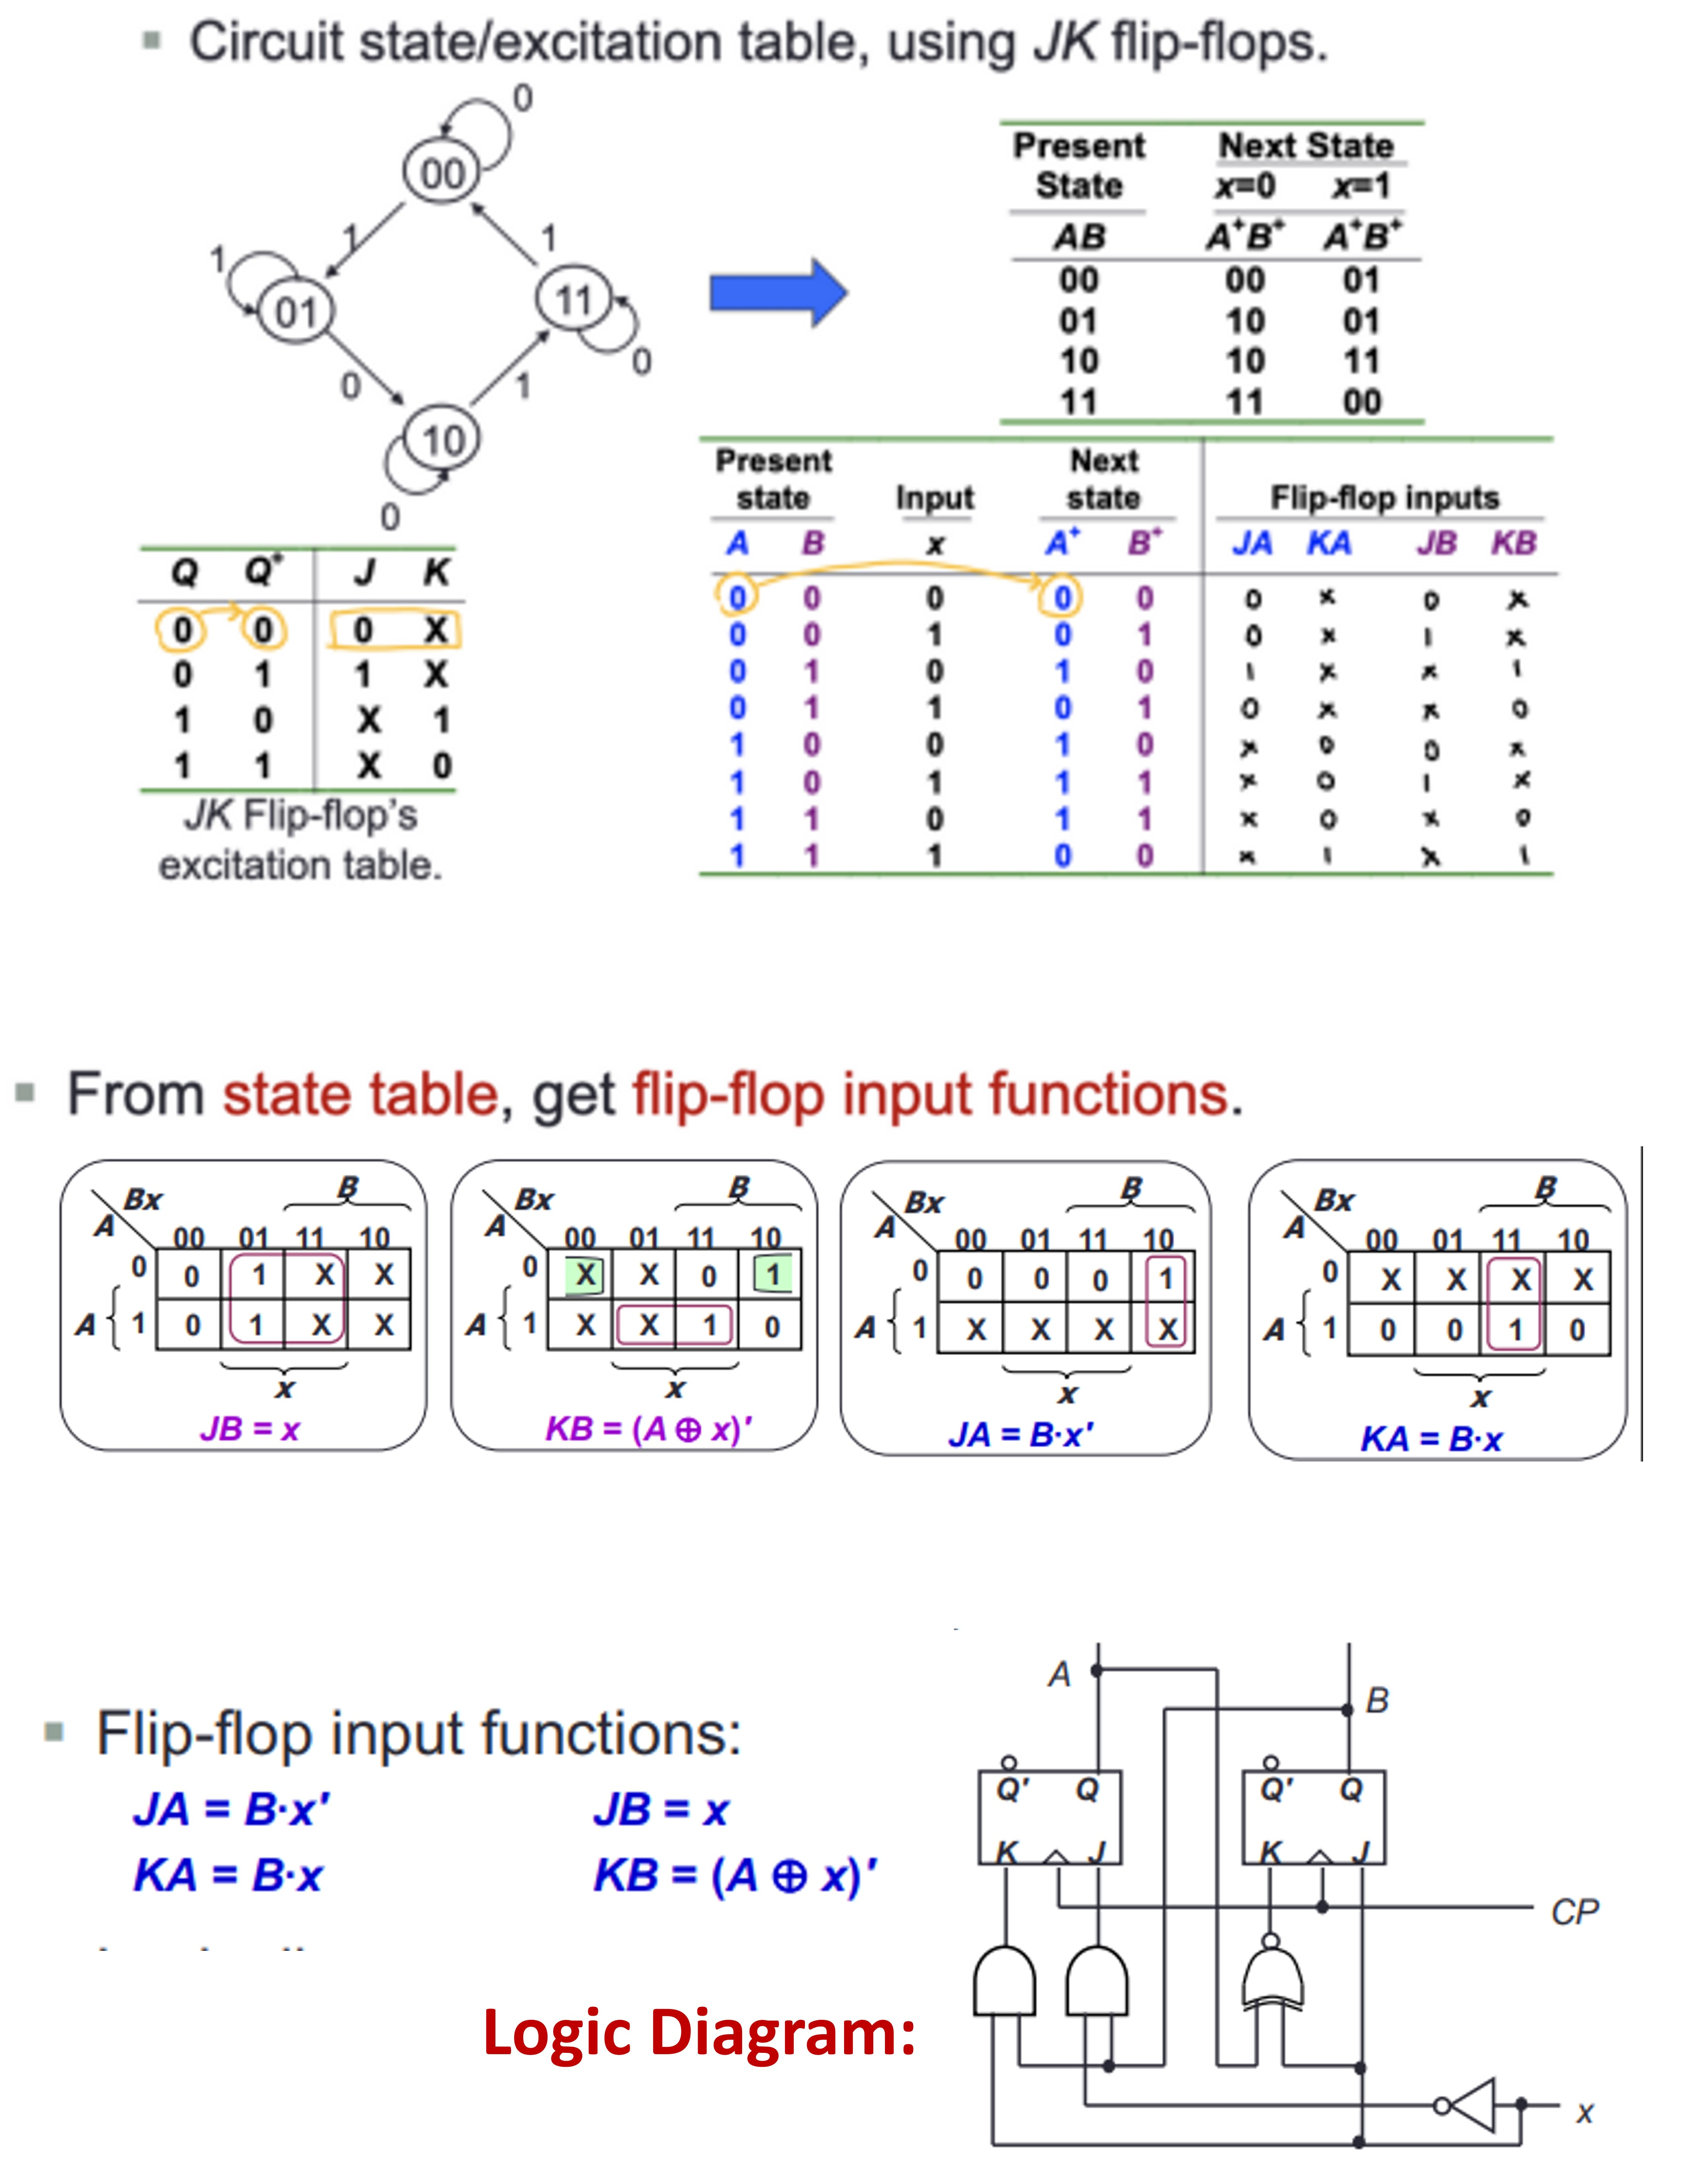
\includegraphics[width=1\linewidth]{sequentialcircuitsdesign}}

\columnbreak

\subsubsection{Unused States}
\begin{itemize}
\item use don't-care for input/next state/flip-flop inputs/output.
\end{itemize}
\centerline{\includegraphics[width=0.8\linewidth]{unusedstates}}


\subsection{Sequential Circuits Analysis}
\textit{(from logic circuit to state equations/table/diagram).}
\begin{enumerate}
\item obtain flip-flop input functions from the circuit
\item fill in the state table (using characteristic table)
\item draw state diagram
\end{enumerate}
\centerline{\includegraphics[width=0.8\linewidth]{analysis}}

\section{18. Memory}
\textbf{Memory}: stores programs and data.
\begin{itemize}
\item 1 byte: 8 bits; 1 word: multiple of bytes, usually size of register
\item memory unit stores binary info in words (groups of bits)
\item data consists of \underline{n lines} for n-bit words
\begin{itemize}
\item \textbf{data input lines}: provide info to write into memory
\item \textbf{data output lines}: carries info to be read from memory
\end{itemize}
\item \textbf{address} consists of \underline{k lines}
\begin{itemize}
\item specifies which word (of the words available) to be selected for
reading/writing
\end{itemize}
\item \textbf{control lines} R/W → specifies dierction of transfer of data
\end{itemize}

\subsubsection{Data Transfer}
\centerline{\includegraphics[width=0.8\linewidth]{Datatransfer}}

\subsubsection{Memory Unit, Read/Write Operations}
\centerline{\includegraphics[width=0.8\linewidth]{memoryunit}}
\textbf{Write}
\begin{itemize}
\item transfers address of the desired word to the address lines
\item transfers the word (data bits) to be stored in memory to the data input lines
\item activates the Write control (set R/W to 0)
\end{itemize}
\textbf{Read}
\begin{itemize}
\item transfers address of the desired word to the address lines
\item activates the Read control (set R/W to 1)
\end{itemize}

\subsubsection{Memory Cell, Memory Array}
\begin{itemize}
\item  \textbf{2 types of RAM}:
\item static RAMs: use flip-flops as the memory cells
\item dynamic RAMs: use capacitor charges to represent data
\item \textbf{Memory Arrays}: array of RAM chips, memory chips combined to form larger memory.
\end{itemize}
\centerline{\includegraphics[width=0.8\linewidth]{memorycell}}


\section{19. MIPS Pipelining}











  
\end{multicols*}
\end{document}